\chapter{研究内容}
\label{chap:contents}

本章では、本研究の内容を説明する。

\section{システム概要}

本システムはセンシングデータを個人でも簡単に利用できるようにすることが目的だ。
そのためのフレームワークを作成し、センシングデータを可視化するという二つの軸をもってシステムを構成した。

以下にシステムの構成を示す。大枠として、Linda\footnote{データをクラウド上で共有するためのフレームワーク。並列処理をしており、同時に多くのクライアントを処理できる。}からサーバーがデータを取得し、クライアントのリクエストに応じて送信する。クライアントでの情報は随時データベースに保存する。

\begin{table}[htbp]
  \caption{システム構成}
  \label{tb:files}
  \begin{center}\begin{tabular}{c|l}
    \hline
    システム&概要\\\hline\hline
    {\tt Linda}&データ元。データストリームからデータを取得する。\\\hline
    {\tt サーバー}&Lindaからデータを取得し、クライアントからのリクエストが来たら送信する。\\\hline
    {\tt クライアント}&サーバーにデータを要求し、ビジュアルプログラミングのビューを提供する。\\\hline
    {\tt データベース}&サーバー、クライアントのデータを保存している。\\\hline
  \end{tabular}\end{center}
\end{table}

\section{データの可視化}
センサーデータを二つの方法で可視化した。

まず一つ目として点滅によるデータの受信だ。Lindaから送られてきたデータを受信するとブロックが青に変化し、元に戻る。(図\ref{fig:image01})
センシングデータを監視してすぐにデータの受信に気付くことができるというメリットがある。\\

\begin{figure}[htbp]
  \begin{minipage}{0.5\hsize}
    \begin{center}
      \fbox{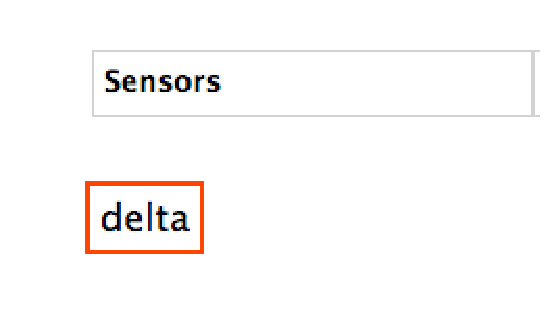
\includegraphics[width=50mm]{image/image1-1.eps}}
    \end{center}
  \end{minipage}
  \begin{minipage}{0.5\hsize}
    \begin{center}
      \fbox{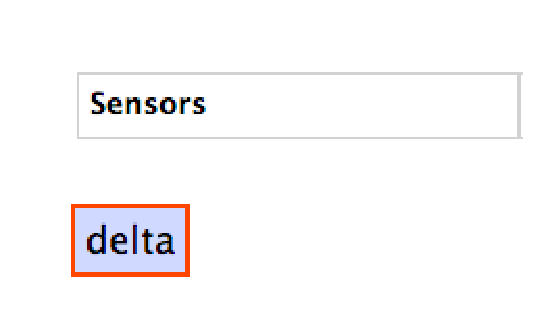
\includegraphics[width=50mm]{image/image1-2.eps}}
    \end{center}
  \end{minipage}
  \caption{点滅でのデータの通知}
  \label{fig:image01}
\end{figure}


そして二つ目として、実際の詳しいデータを見られるようにした。センサーオブジェクトに対してマウスオーバーしてフォーカスすることで実際の数字を表示できるようにした。(図\ref{fig:image02})

\begin{figure}[htbp]
    \begin{center}
       \fbox{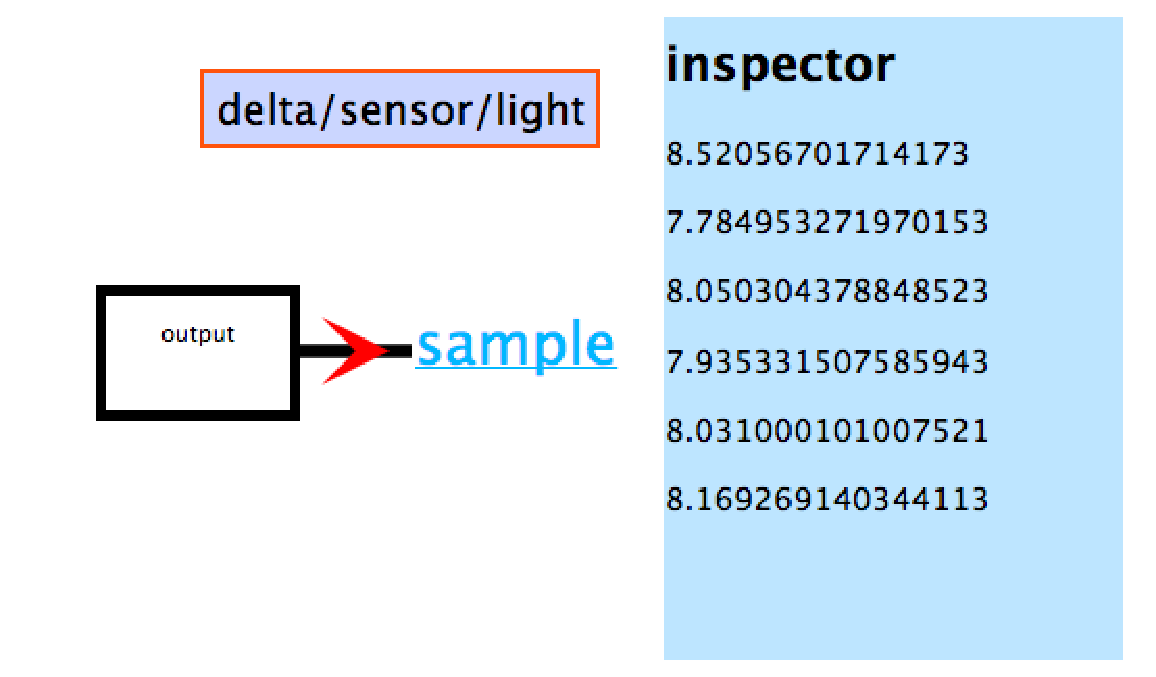
\includegraphics[width=100mm]{image/image02.eps}}
    \end{center}
    \caption{マウスオーバーによるデータの表示}
    \label{fig:image02}
\end{figure}

これら二つの実装により、センシングデータを閲覧する際に自分の欲しい粒度で取得することができるようになった。最低限の実装であれば詳しいデータが見られるだけでもいいが、抽象度を下げて色のみで表現することで閲覧する際の労力を下げることができる。

\section{ビジュアルプログラミング}

ビジュアルプログラミングを実装する際にブロック型のオブジェクトを作成した。以下にオブジェクトごとの解説をする。

\subsection{センサーオブジェクト}

ビジュアルプログラミングをする際には一番最初にセンサーオブジェクトを用意する。このオブジェクトはLindaからのデータを受信し、クライアント側でイベントを作成しデータを受信したら送信するというハブになっている。
また先に述べた通り、センサーデータが来るとこのブロックの点滅、あるいは能動的なデータの取得をすることが可能だ。

\subsection{条件オブジェクト}

センシングデータを扱うための条件オブジェクトを用意した。これにより上限下限、オンオフなどの条件分岐ができる。用意したオブジェクトを以下に列挙する。(図{\ref{fig:max}}〜図{\ref{fig:switch})これらのオブジェクトもブロックとして表現し、条件にマッチするとセンシングデータと同じように点滅する。

\begin{figure}[htbp]
  \begin{minipage}{0.5\hsize}
    \begin{center}
      \fbox{\includegraphics[width=50mm]{image/max.eps}}
    \end{center}
    \caption{Max: 最大値を設定}
    \label{fig:max}
  \end{minipage}
  \begin{minipage}{0.5\hsize}
    \begin{center}
      \fbox{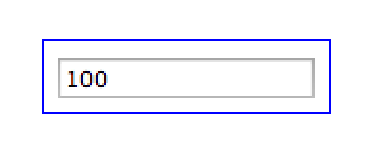
\includegraphics[width=50mm]{image/min.eps}}
    \end{center}
    \caption{min: 最小値を設定}
    \label{fig:min}
  \end{minipage}
\end{figure}

\begin{figure}[htbp]
  \begin{minipage}{0.5\hsize}
    \begin{center}
      \fbox{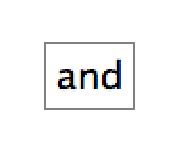
\includegraphics[width=50mm]{image/and.eps}}
    \end{center}
    \caption{and: 論理積を設定}
    \label{fig:and}
  \end{minipage}
  \begin{minipage}{0.5\hsize}
    \begin{center}
      \fbox{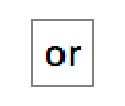
\includegraphics[width=50mm]{image/or.eps}}
    \end{center}
    \caption{or: 論理和を設定}
    \label{fig:or}
  \end{minipage}
\end{figure}

\begin{figure}[htbp]
  \begin{minipage}{0.5\hsize}
    \begin{center}
      \fbox{\includegraphics[width=50mm]{image/switch.eps}}
    \end{center}
    \caption{Switch: on/offを設定}
    \label{fig:switch}
  \end{minipage}
\end{figure}

\subsection{コネクションオブジェクト}

条件オブジェクトと同じ場所にあるが、その中で特殊なオブジェクトがコネクションオブジェクトである。コネクションオブジェクトはブロック間に親子件関係を作成できるオブジェクトである。

コネクションオブジェクトによって親のセンサーデータを条件オブジェクトの持つ自らの条件にかけ、次の世代に受け継ぐということが簡単にプログラムできるようになっている。

例えばdelta/sensor/lightからのセンサーデータかiota/sensor/lightからのセンサーデータがそれぞれ最大値10(10以下)でない場合にsampleというオブジェクトに通知を送るというような設定が簡単にできる。(図{\ref{fig:image03})

\begin{figure}[htbp]
    \begin{center}
       \fbox{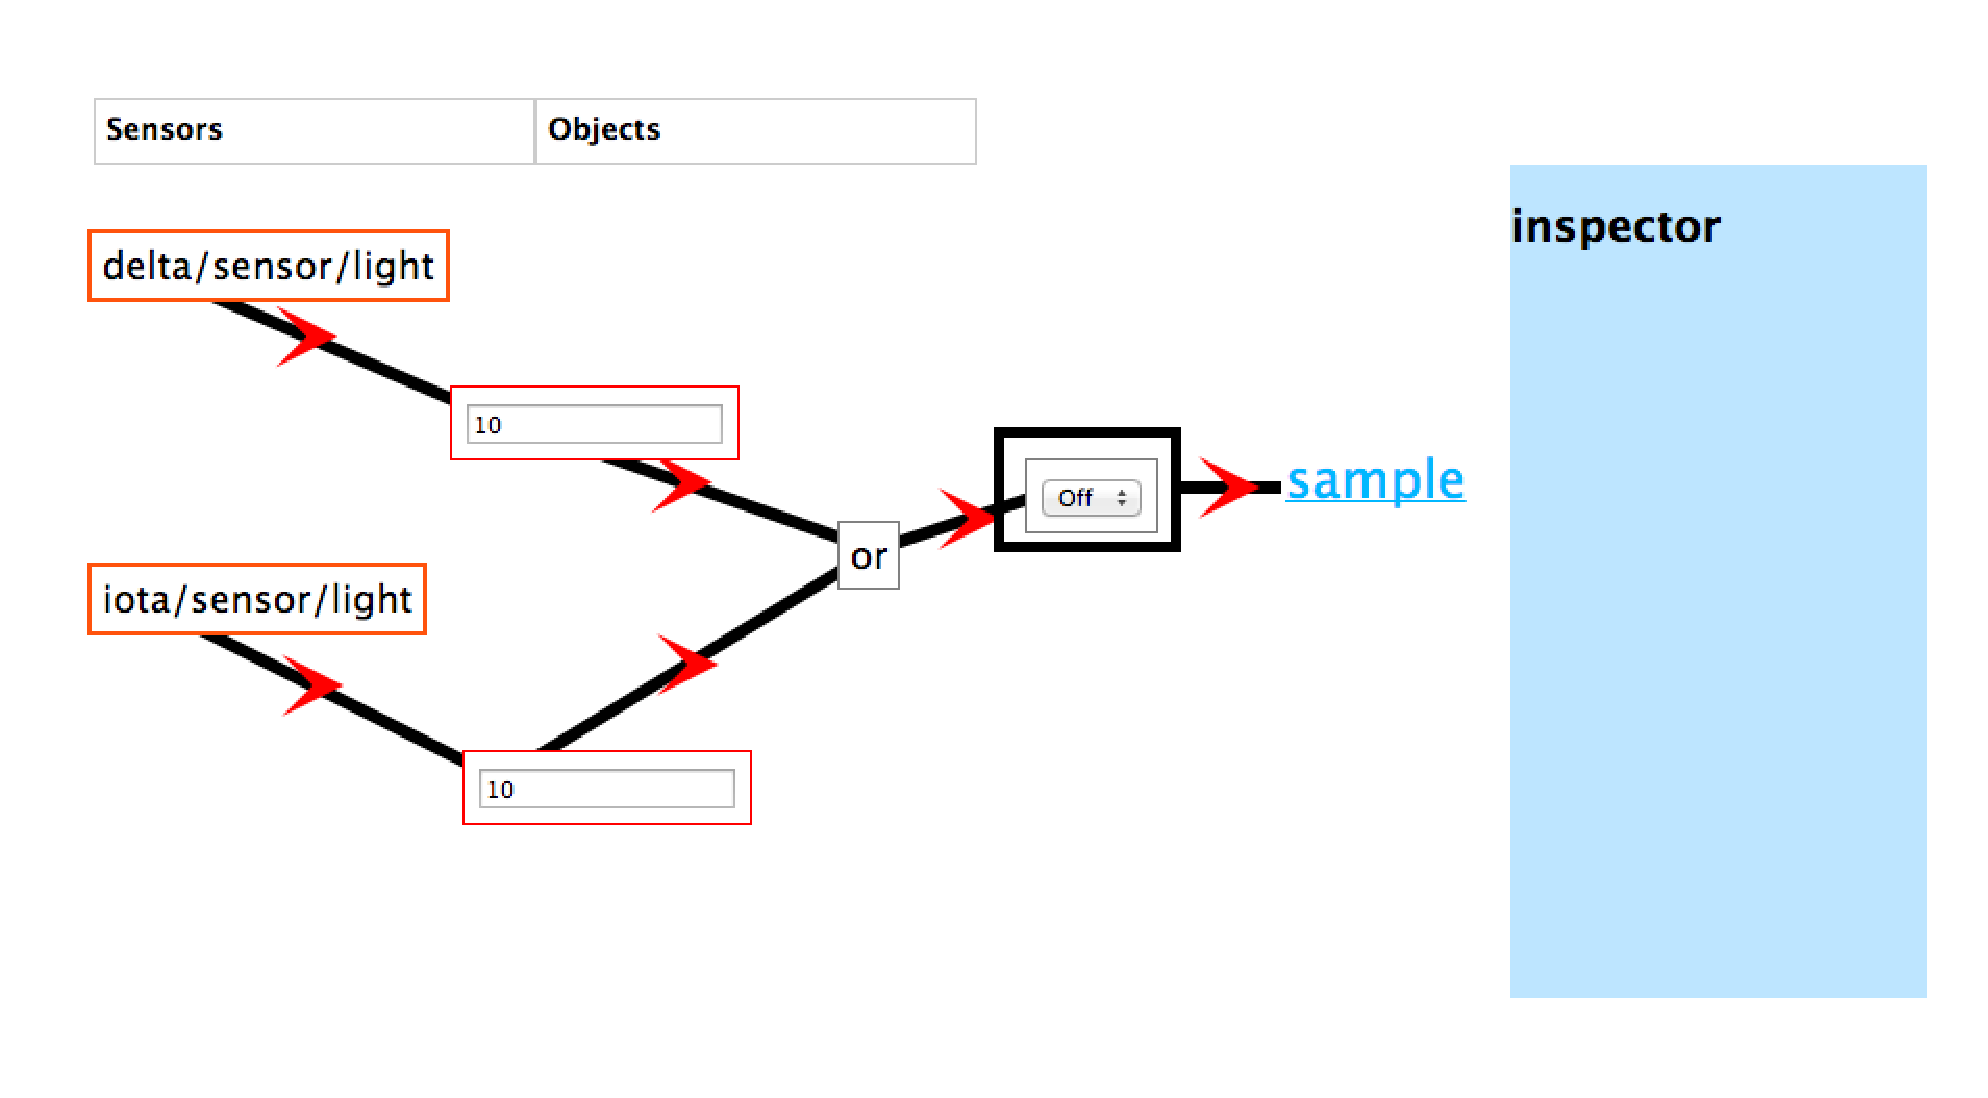
\includegraphics[width=150mm]{image/image03.eps}}
    \end{center}
    \caption{実際にセンシングデータをプログラミングする例}
    \label{fig:image03}
\end{figure}


\subsection{論文情報の設定}
\label{sec:meta}

\begin{itembox}[l]{{\tt main.tex}}
\begin{verbatim}
% 日本語情報(必要なら)
\jclass  {修士論文}                             % 論文種別
\jtitle    {修士論文用 \LaTeX\ テンプレート}    % タイトル。改行する場合は\\を入れる
\juniv    {慶應義塾大学大学院}                  % 大学名
\jfaculty  {政策・メディア研究科}               % 学部、学科
\jauthor  {ほげ山 ふう助}                       % 著者
\jhyear  {24}                                   % 平成○年度
\jsyear  {2012}                                 % 西暦○年度
\jkeyword  {\LaTeX、テンプレート、修士論文}     % 論文のキーワード
\jproject{インタラクションデザインプロジェクト} %プロジェクト名
\jdate{2013年1月}

% 英語情報(必要なら)
\eclass  {Master's Thesis}                            % 論文種別
\etitle    {A \LaTeX Template for Master Thesis}      % タイトル。改行する場合は\\を入れる
\euniv  {Keio University}                             % 大学名
\efaculty  {Graduate School of Media and Governance}  % 学部、学科
\eauthor  {Fusuke Hogeyama}                           % 著者
\eyear  {2012}                                        % 西暦○年度
\ekeyword  {\LaTeX, Templete, Master Thesis}          % 論文のキーワード
\eproject{Interaction Design Project}                 %プロジェクト名
\edate{January 2013}
\end{verbatim}
\end{itembox}

ここでは論文のタイトルや著者の氏名などのメタデータを記述する。ここで書いたデータは、表紙とアブストラクトのページに使われる。必ずしも日本語と英語の両方を設定しなければいけないわけではなくて、自分が必要とする方だけ記述すればよい。

タイトルが長過ぎる場合は、表紙やアブストラクトのページでは自動で折り返して出力される。もし改行位置を自分で指定したい場合は、その場所に \verb|\\| を入力する。


\section{出力}

\verb|\begin{document}| から \verb|\end{document}| に記述した部分が、実際に{\tt DVI}(最終的には{\tt PDF})ファイルとして出力される。

\subsection{外部ファイルの読み込み({\tt include})}

出力部分の具体的な説明の前に、外部ファイルを読み込む方法を説明する。

\verb|\begin{document}| から \verb|\end{document}| の間では、\verb|\include| コマンドを使うことで、別の {\tt *.tex} ファイルを読み込ませられる。

\begin{itembox}[l]{{\tt include}しない場合}
\begin{itembox}[l]{{\tt main.tex}}
\begin{verbatim}
\begin{document}
  \begin{jabstract}
  ほげほげ
  \end{jabstract}
\end{document}
\end{verbatim}
\end{itembox}
\end{itembox}

\begin{itembox}[l]{{\tt include}する場合}
\begin{minipage}{0.5\hsize}
\begin{itembox}[l]{{\tt main.tex}}
\begin{verbatim}
\begin{document}
\chapter{序論}
\label{chap:introduction}
\section{背景}
近年、データのセンシングが簡単になり多くのセンシングデータがビッグデータとしてあふれている。iPhoneやAndroidなどのスマートフォン端末でも位置情報や加速度、傾きなどのデータを常にセンシングすることが出来る。それに伴い、これらのセンシングデータを利用したアプリケーションが出されたり、研究目的として利用されたりするようになった。

しかしながら、これらのセンサーデータを簡単に利用できるようなフレームワークが現状存在しておらずデータをとっても活用せずに終わりといったケースが多かった。使い捨てのデータになっているこれらのデータを活用しない手はないだろう。

また、センサーデータを利用するアプリケーションは多数存在するが、個人がそれらのデータを使っているシーンは少ない。これは個人利用のハードルが高いためだ。多くの場合、プログラミング手段を用いてセンシングデータにアクセスしている。

まずはセンシングデータを可視化することでエンドユーザーに知らせることが必要だ。次点としてセンシングデータを簡単に利用できるように支援する必要がある。

個人が簡単にセンシングデータを利用できるようにするだけでより便利な世の中になるのではないだろうか。

\section{目的}
世の中に氾濫しているセンシングによるビッグデータをより効果的に利用するためのフレームワークを作成する。

そのためにまずはセンシングデータを理解できる数値、文字に変換することが必要になってくる。可視化できていなければどんなデータが利用できるかわからないためだ。

センシングデータを利用するためのフレームワークを作成する。これまでプログラミングができないとセンシングデータを利用できないケースが多くあり課題だったため、プログラミングをせずに使える直感的で使いやすいインタフェースを目指した。GUIでの操作は[1]の研究にもあるようにプログラミングせずに操作する有用な手法であると考えた。

また、他人が作ったセンシングデータをさらに再利用して使えるような仕組み作りをし、汎用的に多くの場面で使えるように想定した。

\section{本文書の構成}
第\ref{chap:introduction}章では本研究の概要を書いた。

第\ref{chap:contents}章では研究内容を説明する。第\ref{chap:prototype}章ではプロトタイプの実装方法を解説する。第\ref{chap:consideration}章では考察を書く。最後に第\ref{chap:conclusion}章にて結論を書き本論文をしめることとする。添付として参考文献を追記する。
 % 01.texをinclude
\end{document}
\end{verbatim}
\end{itembox}
\end{minipage}
\begin{minipage}{0.5\hsize}
\begin{itembox}[l]{{\tt 01.tex}}
\begin{verbatim}
\begin{jabstract}
ほげほげ
\end{jabstract}
\end{verbatim}
\end{itembox}
\end{minipage}
\end{itembox}

{\tt include}しない場合とする場合を比較するとこのとおり。どちらも出力結果は一緒。{\tt include}する場合は、読み込ませたい箇所に、読み込ませたい{\tt *.tex}ファイルの名前を、拡張子を除いて \verb|\include| コマンドで書けばよい。

\verb|\include| コマンドを用いるか用いないかは、たぶん文書量や個人の好みに依る。例えば章ごとに別のファイルにしておけば、修正箇所を探すときの手間が多少は省けるかもしれない。Gitで人と共有しつつ校正を頼むときにもファイルが分かれていたほうがコンフリクトを起こしにくい。


\subsection{表紙の出力}

\begin{itembox}[l]{{\tt main.tex}}
\begin{verbatim}
\ifjapanese
  \jmaketitle    % 表紙(日本語)
\else
  \emaketitle    % 表紙(英語)
\fi
\end{verbatim}
\end{itembox}

最初に、表紙を出力する。

\verb|\jmaketitle| が実行されると日本語の表紙が、\verb|\emaketitle| が実行されると英語の表紙がそれぞれ出力される。日本語の表紙には、第\ref{sec:meta}節で設定したうちの日本語の情報が、英語の表紙には同節で設定したうち英語の情報が、それぞれ参照されて、表記される。

デフォルトでは第\ref{sec:lang}説で設定した言語の表紙のみが出力されるようになっている。

\subsection{アブストラクトの出力}

\begin{itembox}[l]{{\tt main.tex}}
\begin{verbatim}
% ■ アブストラクトの出力 ■
%	◆書式:
%		begin{jabstract}〜end{jabstract}	:日本語のアブストラクト
%		begin{eabstract}〜end{eabstract}	:英語のアブストラクト
%		※ 不要ならばコマンドごと消せば出力されない。



% 日本語のアブストラクト
\begin{jabstract}
  近年、高性能のセンサーと豊富なリソースにより、iPhoneなどの端末で個人でも簡単にセンシングデータを取得できるようになった。加速度、傾き、位置情報など、多くのデータがビッグデータとしてあふれている。多くのデータはそれぞれが価値を持っているがそれらのデータを簡単に利用するフレームワークが現段階では存在しない。
そこで本研究ではセンシングデータを可視化し、データを簡単に取り出して利用できるフレームワークを作成した。本研究ではLindaという分散型プログラミングができるフレーワークを拡張した形になっている。Lindaは様々な場所で様々なユーザーが取得したセンシングデータをWeb上に流し、誰でも共有して利用できるようにしている。それらのセンシングデータをより簡単に利用できるようにすることで多くのプロダクトが産まれる可能性が広がるだろう。
  また、本研究ではセンシングデータを物に結びつけてプッシュAPI化する実装となっている。センシングデータを物と結びつけることでよりモジュール化し、より直感的に再利用できるメリットがある。

\end{jabstract}



% 英語のアブストラクト
	% アブストラクト。要独自コマンド、include先参照のこと
\end{verbatim}
\end{itembox}

表紙の次は、アブストラクト。

アブストラクトを出力するには、出力したい位置に、指定のコマンドを用いて文章を書き下せばよい。{\tt main.tex}に直接書いてもよいし、先述した \verb|\include| コマンドを利用して{\tt include}してもよい。

\verb|\begin{jabstract}| から \verb|\end{jabstract}| の間に書いた文章が日本語のアブストラクトとして、\verb|\begin{eabstract}| から \verb|\end{eabstract}| の間に書いた文章が英語のアブストラクトとして、それぞれ独立したページに出力される。

アブストラクトのページには、論文のタイトルやキーワードなどが、第\ref{sec:meta}節で設定した情報をもとにして自動で表記される。

日本語か英語のどちらか一方のみでよい場合は、不要な言語の方のコマンドを削除すればよい。これは、\verb|\begin| と \verb|\end| というコマンド自身も含めて削除する、ということで、\verb|\begin| と \verb|\end| の間を空っぽにするという意味ではないので注意。



\subsection{目次類の出力}
\label{sec:toc}

\begin{itembox}[l]{{\tt main.tex}}
\begin{verbatim}
\tableofcontents	% 目次
\listoffigures		% 表目次
\listoftables		% 図目次
\end{verbatim}
\end{itembox}

アブストラクトの次に、目次。文書の目次、図の目次、表の目次の三種類。

目次類を出力するには、出力したい位置に指定のコマンドを書けばよい。

これらのコマンドは、コンパイル時点での一時ファイル\footnote{{\tt *.toc}、{\tt *.lof}、{\tt *.lot}}の情報を、目次として体裁を整えて出力するもの。一時ファイルは、\verb|\begin{document}| から \verb|\end{document}| の間の章や節、図や表をコンパイルするときに、ついでに情報を取得しておいて生成される。

つまり気をつけなければいけないのは、コンパイルを一回しただけでは、一時ファイルが最新の状態に更新されるだけで、肝心の目次は正しい情報では出力されないということ。目次類を正しい情報で出力するには、最低二回のコンパイルが必要。一回目のコンパイルで一時ファイルが最新の情報に更新されて、二回目のコンパイルで初めて、その最新の一時ファイルの情報をもとに目次が出力される。

だから、文書に何らかの修正をして保存したあとは、最低でも二回、連続してコンパイルしないといけないことに注意する。

図や表を一つも使用していない場合は、目次名のみが書かれた空白のページが出力される。もしこれが不要な場合は、該当するコマンドをコメントアウトすればよい。


\subsection{本文の出力}

\begin{itembox}[l]{{\tt main.tex}}
\begin{verbatim}
\chapter{序論}
\label{chap:introduction}
\section{背景}
近年、データのセンシングが簡単になり多くのセンシングデータがビッグデータとしてあふれている。iPhoneやAndroidなどのスマートフォン端末でも位置情報や加速度、傾きなどのデータを常にセンシングすることが出来る。それに伴い、これらのセンシングデータを利用したアプリケーションが出されたり、研究目的として利用されたりするようになった。

しかしながら、これらのセンサーデータを簡単に利用できるようなフレームワークが現状存在しておらずデータをとっても活用せずに終わりといったケースが多かった。使い捨てのデータになっているこれらのデータを活用しない手はないだろう。

また、センサーデータを利用するアプリケーションは多数存在するが、個人がそれらのデータを使っているシーンは少ない。これは個人利用のハードルが高いためだ。多くの場合、プログラミング手段を用いてセンシングデータにアクセスしている。

まずはセンシングデータを可視化することでエンドユーザーに知らせることが必要だ。次点としてセンシングデータを簡単に利用できるように支援する必要がある。

個人が簡単にセンシングデータを利用できるようにするだけでより便利な世の中になるのではないだろうか。

\section{目的}
世の中に氾濫しているセンシングによるビッグデータをより効果的に利用するためのフレームワークを作成する。

そのためにまずはセンシングデータを理解できる数値、文字に変換することが必要になってくる。可視化できていなければどんなデータが利用できるかわからないためだ。

センシングデータを利用するためのフレームワークを作成する。これまでプログラミングができないとセンシングデータを利用できないケースが多くあり課題だったため、プログラミングをせずに使える直感的で使いやすいインタフェースを目指した。GUIでの操作は[1]の研究にもあるようにプログラミングせずに操作する有用な手法であると考えた。

また、他人が作ったセンシングデータをさらに再利用して使えるような仕組み作りをし、汎用的に多くの場面で使えるように想定した。

\section{本文書の構成}
第\ref{chap:introduction}章では本研究の概要を書いた。

第\ref{chap:contents}章では研究内容を説明する。第\ref{chap:prototype}章ではプロトタイプの実装方法を解説する。第\ref{chap:consideration}章では考察を書く。最後に第\ref{chap:conclusion}章にて結論を書き本論文をしめることとする。添付として参考文献を追記する。
	% 本文1
\chapter{研究内容}
\label{chap:contents}

本章では、本研究の内容を説明する。

\section{システム概要}

本システムはセンシングデータを個人でも簡単に利用できるようにすることが目的だ。
そのためのフレームワークを作成し、センシングデータを可視化するという二つの軸をもってシステムを構成した。

以下にシステムの構成を示す。大枠として、Linda\footnote{データをクラウド上で共有するためのフレームワーク。並列処理をしており、同時に多くのクライアントを処理できる。}からサーバーがデータを取得し、クライアントのリクエストに応じて送信する。クライアントでの情報は随時データベースに保存する。

\begin{table}[htbp]
  \caption{システム構成}
  \label{tb:files}
  \begin{center}\begin{tabular}{c|l}
    \hline
    システム&概要\\\hline\hline
    {\tt Linda}&データ元。データストリームからデータを取得する。\\\hline
    {\tt サーバー}&Lindaからデータを取得し、クライアントからのリクエストが来たら送信する。\\\hline
    {\tt クライアント}&サーバーにデータを要求し、ビジュアルプログラミングのビューを提供する。\\\hline
    {\tt データベース}&サーバー、クライアントのデータを保存している。\\\hline
  \end{tabular}\end{center}
\end{table}

\section{データの可視化}
センサーデータを二つの方法で可視化した。

まず一つ目として点滅によるデータの受信だ。Lindaから送られてきたデータを受信するとブロックが青に変化し、元に戻る。(図\ref{fig:image01})
センシングデータを監視してすぐにデータの受信に気付くことができるというメリットがある。\\

\begin{figure}[htbp]
  \begin{minipage}{0.5\hsize}
    \begin{center}
      \fbox{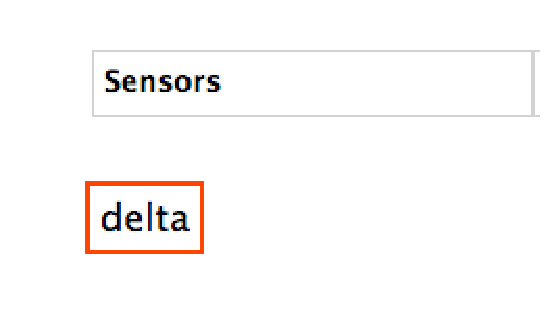
\includegraphics[width=50mm]{image/image1-1.eps}}
    \end{center}
  \end{minipage}
  \begin{minipage}{0.5\hsize}
    \begin{center}
      \fbox{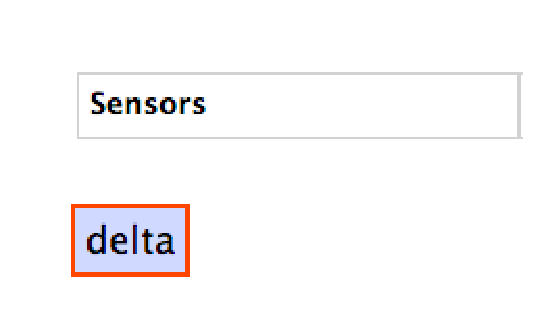
\includegraphics[width=50mm]{image/image1-2.eps}}
    \end{center}
  \end{minipage}
  \caption{点滅でのデータの通知}
  \label{fig:image01}
\end{figure}


そして二つ目として、実際の詳しいデータを見られるようにした。センサーオブジェクトに対してマウスオーバーしてフォーカスすることで実際の数字を表示できるようにした。(図\ref{fig:image02})

\begin{figure}[htbp]
    \begin{center}
       \fbox{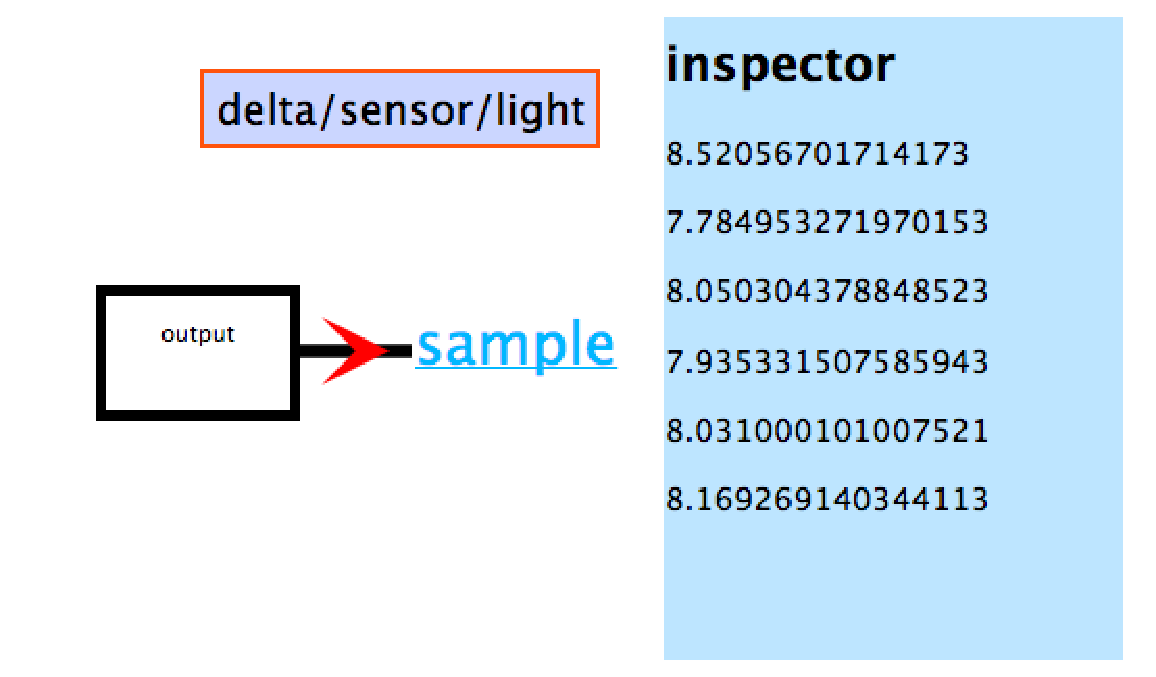
\includegraphics[width=100mm]{image/image02.eps}}
    \end{center}
    \caption{マウスオーバーによるデータの表示}
    \label{fig:image02}
\end{figure}

これら二つの実装により、センシングデータを閲覧する際に自分の欲しい粒度で取得することができるようになった。最低限の実装であれば詳しいデータが見られるだけでもいいが、抽象度を下げて色のみで表現することで閲覧する際の労力を下げることができる。

\section{ビジュアルプログラミング}

ビジュアルプログラミングを実装する際にブロック型のオブジェクトを作成した。以下にオブジェクトごとの解説をする。

\subsection{センサーオブジェクト}

ビジュアルプログラミングをする際には一番最初にセンサーオブジェクトを用意する。このオブジェクトはLindaからのデータを受信し、クライアント側でイベントを作成しデータを受信したら送信するというハブになっている。
また先に述べた通り、センサーデータが来るとこのブロックの点滅、あるいは能動的なデータの取得をすることが可能だ。

\subsection{条件オブジェクト}

センシングデータを扱うための条件オブジェクトを用意した。これにより上限下限、オンオフなどの条件分岐ができる。用意したオブジェクトを以下に列挙する。(図{\ref{fig:max}}〜図{\ref{fig:switch})これらのオブジェクトもブロックとして表現し、条件にマッチするとセンシングデータと同じように点滅する。

\begin{figure}[htbp]
  \begin{minipage}{0.5\hsize}
    \begin{center}
      \fbox{\includegraphics[width=50mm]{image/max.eps}}
    \end{center}
    \caption{Max: 最大値を設定}
    \label{fig:max}
  \end{minipage}
  \begin{minipage}{0.5\hsize}
    \begin{center}
      \fbox{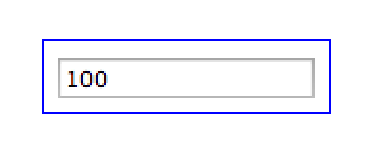
\includegraphics[width=50mm]{image/min.eps}}
    \end{center}
    \caption{min: 最小値を設定}
    \label{fig:min}
  \end{minipage}
\end{figure}

\begin{figure}[htbp]
  \begin{minipage}{0.5\hsize}
    \begin{center}
      \fbox{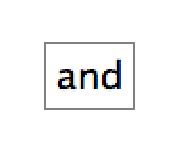
\includegraphics[width=50mm]{image/and.eps}}
    \end{center}
    \caption{and: 論理積を設定}
    \label{fig:and}
  \end{minipage}
  \begin{minipage}{0.5\hsize}
    \begin{center}
      \fbox{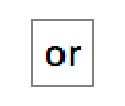
\includegraphics[width=50mm]{image/or.eps}}
    \end{center}
    \caption{or: 論理和を設定}
    \label{fig:or}
  \end{minipage}
\end{figure}

\begin{figure}[htbp]
  \begin{minipage}{0.5\hsize}
    \begin{center}
      \fbox{\includegraphics[width=50mm]{image/switch.eps}}
    \end{center}
    \caption{Switch: on/offを設定}
    \label{fig:switch}
  \end{minipage}
\end{figure}

\subsection{コネクションオブジェクト}

条件オブジェクトと同じ場所にあるが、その中で特殊なオブジェクトがコネクションオブジェクトである。コネクションオブジェクトはブロック間に親子件関係を作成できるオブジェクトである。

コネクションオブジェクトによって親のセンサーデータを条件オブジェクトの持つ自らの条件にかけ、次の世代に受け継ぐということが簡単にプログラムできるようになっている。

例えばdelta/sensor/lightからのセンサーデータかiota/sensor/lightからのセンサーデータがそれぞれ最大値10(10以下)でない場合にsampleというオブジェクトに通知を送るというような設定が簡単にできる。(図{\ref{fig:image03})

\begin{figure}[htbp]
    \begin{center}
       \fbox{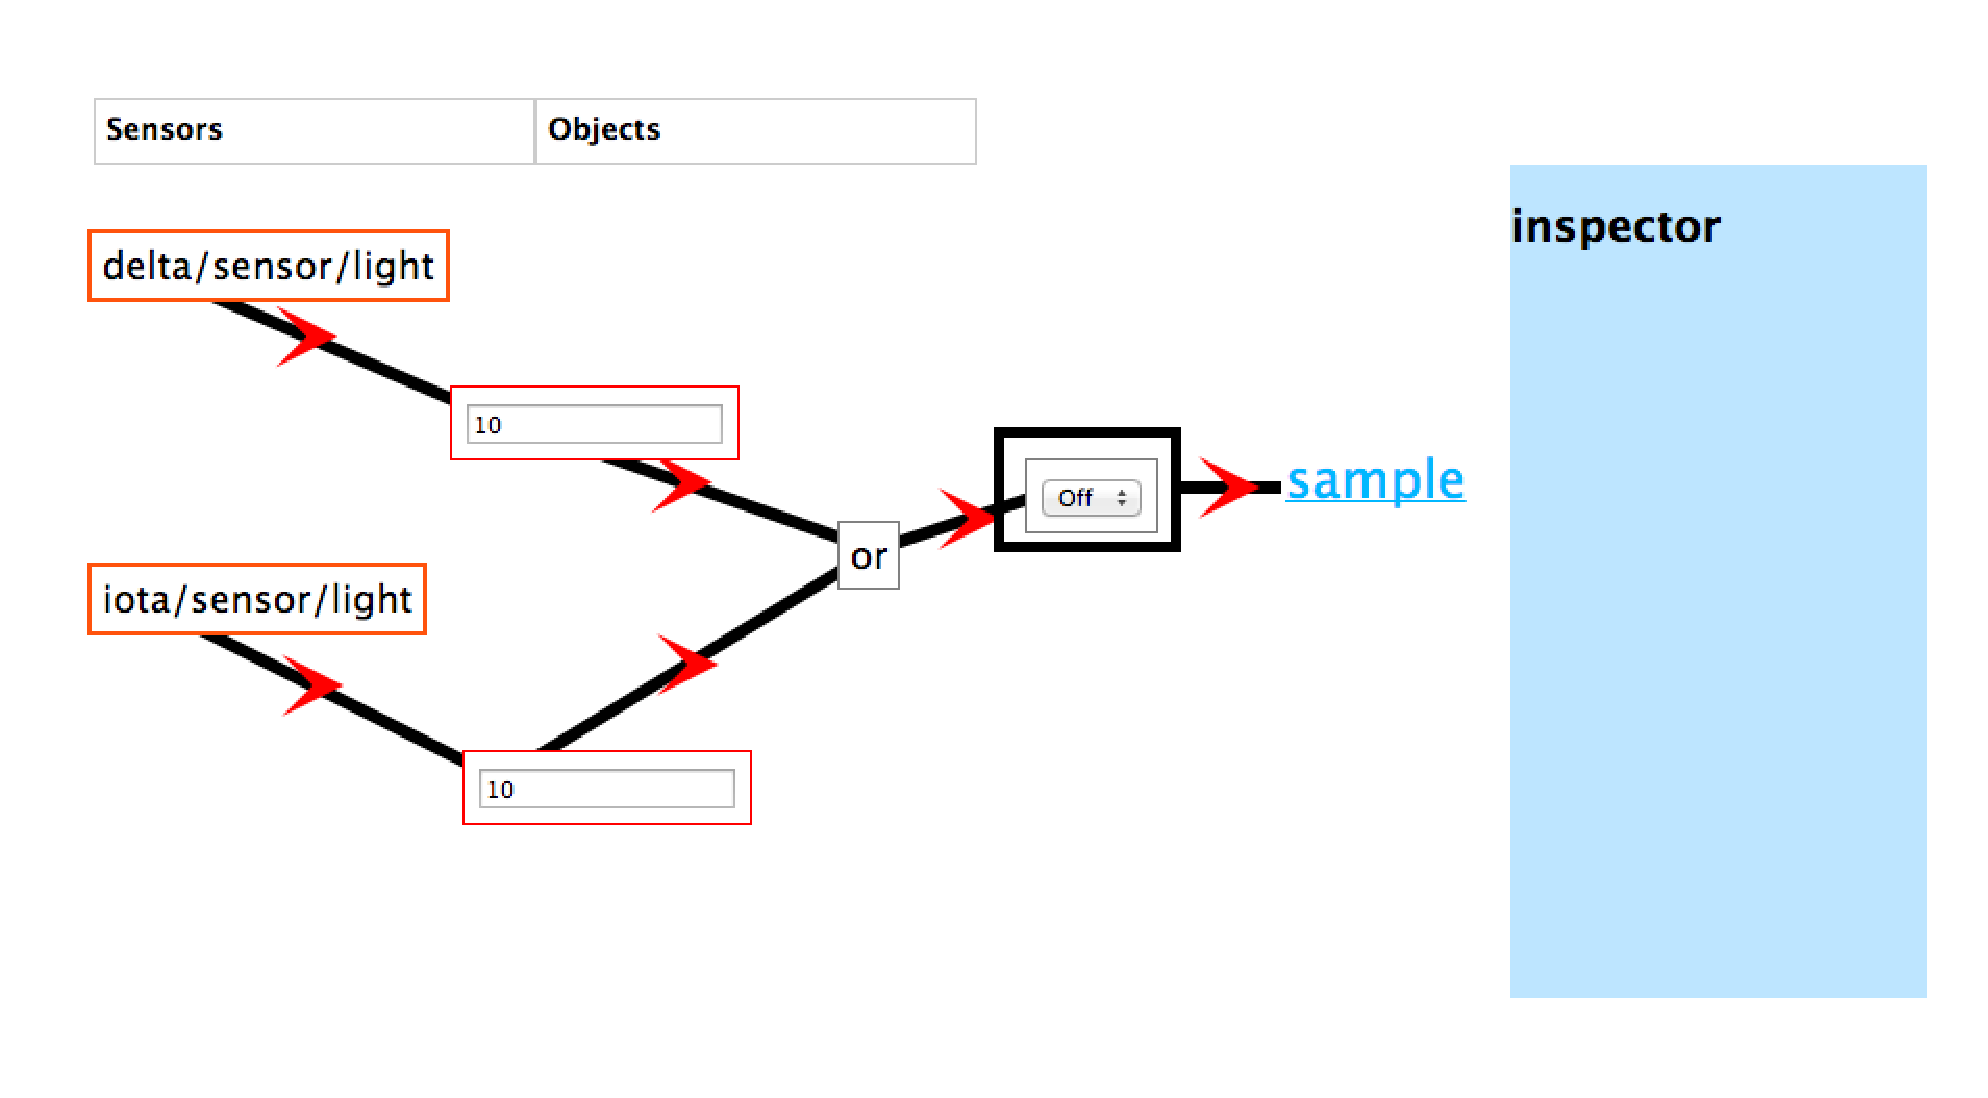
\includegraphics[width=150mm]{image/image03.eps}}
    \end{center}
    \caption{実際にセンシングデータをプログラミングする例}
    \label{fig:image03}
\end{figure}


\subsection{論文情報の設定}
\label{sec:meta}

\begin{itembox}[l]{{\tt main.tex}}
\begin{verbatim}
% 日本語情報(必要なら)
\jclass  {修士論文}                             % 論文種別
\jtitle    {修士論文用 \LaTeX\ テンプレート}    % タイトル。改行する場合は\\を入れる
\juniv    {慶應義塾大学大学院}                  % 大学名
\jfaculty  {政策・メディア研究科}               % 学部、学科
\jauthor  {ほげ山 ふう助}                       % 著者
\jhyear  {24}                                   % 平成○年度
\jsyear  {2012}                                 % 西暦○年度
\jkeyword  {\LaTeX、テンプレート、修士論文}     % 論文のキーワード
\jproject{インタラクションデザインプロジェクト} %プロジェクト名
\jdate{2013年1月}

% 英語情報(必要なら)
\eclass  {Master's Thesis}                            % 論文種別
\etitle    {A \LaTeX Template for Master Thesis}      % タイトル。改行する場合は\\を入れる
\euniv  {Keio University}                             % 大学名
\efaculty  {Graduate School of Media and Governance}  % 学部、学科
\eauthor  {Fusuke Hogeyama}                           % 著者
\eyear  {2012}                                        % 西暦○年度
\ekeyword  {\LaTeX, Templete, Master Thesis}          % 論文のキーワード
\eproject{Interaction Design Project}                 %プロジェクト名
\edate{January 2013}
\end{verbatim}
\end{itembox}

ここでは論文のタイトルや著者の氏名などのメタデータを記述する。ここで書いたデータは、表紙とアブストラクトのページに使われる。必ずしも日本語と英語の両方を設定しなければいけないわけではなくて、自分が必要とする方だけ記述すればよい。

タイトルが長過ぎる場合は、表紙やアブストラクトのページでは自動で折り返して出力される。もし改行位置を自分で指定したい場合は、その場所に \verb|\\| を入力する。


\section{出力}

\verb|\begin{document}| から \verb|\end{document}| に記述した部分が、実際に{\tt DVI}(最終的には{\tt PDF})ファイルとして出力される。

\subsection{外部ファイルの読み込み({\tt include})}

出力部分の具体的な説明の前に、外部ファイルを読み込む方法を説明する。

\verb|\begin{document}| から \verb|\end{document}| の間では、\verb|\include| コマンドを使うことで、別の {\tt *.tex} ファイルを読み込ませられる。

\begin{itembox}[l]{{\tt include}しない場合}
\begin{itembox}[l]{{\tt main.tex}}
\begin{verbatim}
\begin{document}
  \begin{jabstract}
  ほげほげ
  \end{jabstract}
\end{document}
\end{verbatim}
\end{itembox}
\end{itembox}

\begin{itembox}[l]{{\tt include}する場合}
\begin{minipage}{0.5\hsize}
\begin{itembox}[l]{{\tt main.tex}}
\begin{verbatim}
\begin{document}
\chapter{序論}
\label{chap:introduction}
\section{背景}
近年、データのセンシングが簡単になり多くのセンシングデータがビッグデータとしてあふれている。iPhoneやAndroidなどのスマートフォン端末でも位置情報や加速度、傾きなどのデータを常にセンシングすることが出来る。それに伴い、これらのセンシングデータを利用したアプリケーションが出されたり、研究目的として利用されたりするようになった。

しかしながら、これらのセンサーデータを簡単に利用できるようなフレームワークが現状存在しておらずデータをとっても活用せずに終わりといったケースが多かった。使い捨てのデータになっているこれらのデータを活用しない手はないだろう。

また、センサーデータを利用するアプリケーションは多数存在するが、個人がそれらのデータを使っているシーンは少ない。これは個人利用のハードルが高いためだ。多くの場合、プログラミング手段を用いてセンシングデータにアクセスしている。

まずはセンシングデータを可視化することでエンドユーザーに知らせることが必要だ。次点としてセンシングデータを簡単に利用できるように支援する必要がある。

個人が簡単にセンシングデータを利用できるようにするだけでより便利な世の中になるのではないだろうか。

\section{目的}
世の中に氾濫しているセンシングによるビッグデータをより効果的に利用するためのフレームワークを作成する。

そのためにまずはセンシングデータを理解できる数値、文字に変換することが必要になってくる。可視化できていなければどんなデータが利用できるかわからないためだ。

センシングデータを利用するためのフレームワークを作成する。これまでプログラミングができないとセンシングデータを利用できないケースが多くあり課題だったため、プログラミングをせずに使える直感的で使いやすいインタフェースを目指した。GUIでの操作は[1]の研究にもあるようにプログラミングせずに操作する有用な手法であると考えた。

また、他人が作ったセンシングデータをさらに再利用して使えるような仕組み作りをし、汎用的に多くの場面で使えるように想定した。

\section{本文書の構成}
第\ref{chap:introduction}章では本研究の概要を書いた。

第\ref{chap:contents}章では研究内容を説明する。第\ref{chap:prototype}章ではプロトタイプの実装方法を解説する。第\ref{chap:consideration}章では考察を書く。最後に第\ref{chap:conclusion}章にて結論を書き本論文をしめることとする。添付として参考文献を追記する。
 % 01.texをinclude
\end{document}
\end{verbatim}
\end{itembox}
\end{minipage}
\begin{minipage}{0.5\hsize}
\begin{itembox}[l]{{\tt 01.tex}}
\begin{verbatim}
\begin{jabstract}
ほげほげ
\end{jabstract}
\end{verbatim}
\end{itembox}
\end{minipage}
\end{itembox}

{\tt include}しない場合とする場合を比較するとこのとおり。どちらも出力結果は一緒。{\tt include}する場合は、読み込ませたい箇所に、読み込ませたい{\tt *.tex}ファイルの名前を、拡張子を除いて \verb|\include| コマンドで書けばよい。

\verb|\include| コマンドを用いるか用いないかは、たぶん文書量や個人の好みに依る。例えば章ごとに別のファイルにしておけば、修正箇所を探すときの手間が多少は省けるかもしれない。Gitで人と共有しつつ校正を頼むときにもファイルが分かれていたほうがコンフリクトを起こしにくい。


\subsection{表紙の出力}

\begin{itembox}[l]{{\tt main.tex}}
\begin{verbatim}
\ifjapanese
  \jmaketitle    % 表紙(日本語)
\else
  \emaketitle    % 表紙(英語)
\fi
\end{verbatim}
\end{itembox}

最初に、表紙を出力する。

\verb|\jmaketitle| が実行されると日本語の表紙が、\verb|\emaketitle| が実行されると英語の表紙がそれぞれ出力される。日本語の表紙には、第\ref{sec:meta}節で設定したうちの日本語の情報が、英語の表紙には同節で設定したうち英語の情報が、それぞれ参照されて、表記される。

デフォルトでは第\ref{sec:lang}説で設定した言語の表紙のみが出力されるようになっている。

\subsection{アブストラクトの出力}

\begin{itembox}[l]{{\tt main.tex}}
\begin{verbatim}
% ■ アブストラクトの出力 ■
%	◆書式:
%		begin{jabstract}〜end{jabstract}	:日本語のアブストラクト
%		begin{eabstract}〜end{eabstract}	:英語のアブストラクト
%		※ 不要ならばコマンドごと消せば出力されない。



% 日本語のアブストラクト
\begin{jabstract}
  近年、高性能のセンサーと豊富なリソースにより、iPhoneなどの端末で個人でも簡単にセンシングデータを取得できるようになった。加速度、傾き、位置情報など、多くのデータがビッグデータとしてあふれている。多くのデータはそれぞれが価値を持っているがそれらのデータを簡単に利用するフレームワークが現段階では存在しない。
そこで本研究ではセンシングデータを可視化し、データを簡単に取り出して利用できるフレームワークを作成した。本研究ではLindaという分散型プログラミングができるフレーワークを拡張した形になっている。Lindaは様々な場所で様々なユーザーが取得したセンシングデータをWeb上に流し、誰でも共有して利用できるようにしている。それらのセンシングデータをより簡単に利用できるようにすることで多くのプロダクトが産まれる可能性が広がるだろう。
  また、本研究ではセンシングデータを物に結びつけてプッシュAPI化する実装となっている。センシングデータを物と結びつけることでよりモジュール化し、より直感的に再利用できるメリットがある。

\end{jabstract}



% 英語のアブストラクト
	% アブストラクト。要独自コマンド、include先参照のこと
\end{verbatim}
\end{itembox}

表紙の次は、アブストラクト。

アブストラクトを出力するには、出力したい位置に、指定のコマンドを用いて文章を書き下せばよい。{\tt main.tex}に直接書いてもよいし、先述した \verb|\include| コマンドを利用して{\tt include}してもよい。

\verb|\begin{jabstract}| から \verb|\end{jabstract}| の間に書いた文章が日本語のアブストラクトとして、\verb|\begin{eabstract}| から \verb|\end{eabstract}| の間に書いた文章が英語のアブストラクトとして、それぞれ独立したページに出力される。

アブストラクトのページには、論文のタイトルやキーワードなどが、第\ref{sec:meta}節で設定した情報をもとにして自動で表記される。

日本語か英語のどちらか一方のみでよい場合は、不要な言語の方のコマンドを削除すればよい。これは、\verb|\begin| と \verb|\end| というコマンド自身も含めて削除する、ということで、\verb|\begin| と \verb|\end| の間を空っぽにするという意味ではないので注意。



\subsection{目次類の出力}
\label{sec:toc}

\begin{itembox}[l]{{\tt main.tex}}
\begin{verbatim}
\tableofcontents	% 目次
\listoffigures		% 表目次
\listoftables		% 図目次
\end{verbatim}
\end{itembox}

アブストラクトの次に、目次。文書の目次、図の目次、表の目次の三種類。

目次類を出力するには、出力したい位置に指定のコマンドを書けばよい。

これらのコマンドは、コンパイル時点での一時ファイル\footnote{{\tt *.toc}、{\tt *.lof}、{\tt *.lot}}の情報を、目次として体裁を整えて出力するもの。一時ファイルは、\verb|\begin{document}| から \verb|\end{document}| の間の章や節、図や表をコンパイルするときに、ついでに情報を取得しておいて生成される。

つまり気をつけなければいけないのは、コンパイルを一回しただけでは、一時ファイルが最新の状態に更新されるだけで、肝心の目次は正しい情報では出力されないということ。目次類を正しい情報で出力するには、最低二回のコンパイルが必要。一回目のコンパイルで一時ファイルが最新の情報に更新されて、二回目のコンパイルで初めて、その最新の一時ファイルの情報をもとに目次が出力される。

だから、文書に何らかの修正をして保存したあとは、最低でも二回、連続してコンパイルしないといけないことに注意する。

図や表を一つも使用していない場合は、目次名のみが書かれた空白のページが出力される。もしこれが不要な場合は、該当するコマンドをコメントアウトすればよい。


\subsection{本文の出力}

\begin{itembox}[l]{{\tt main.tex}}
\begin{verbatim}
\chapter{序論}
\label{chap:introduction}
\section{背景}
近年、データのセンシングが簡単になり多くのセンシングデータがビッグデータとしてあふれている。iPhoneやAndroidなどのスマートフォン端末でも位置情報や加速度、傾きなどのデータを常にセンシングすることが出来る。それに伴い、これらのセンシングデータを利用したアプリケーションが出されたり、研究目的として利用されたりするようになった。

しかしながら、これらのセンサーデータを簡単に利用できるようなフレームワークが現状存在しておらずデータをとっても活用せずに終わりといったケースが多かった。使い捨てのデータになっているこれらのデータを活用しない手はないだろう。

また、センサーデータを利用するアプリケーションは多数存在するが、個人がそれらのデータを使っているシーンは少ない。これは個人利用のハードルが高いためだ。多くの場合、プログラミング手段を用いてセンシングデータにアクセスしている。

まずはセンシングデータを可視化することでエンドユーザーに知らせることが必要だ。次点としてセンシングデータを簡単に利用できるように支援する必要がある。

個人が簡単にセンシングデータを利用できるようにするだけでより便利な世の中になるのではないだろうか。

\section{目的}
世の中に氾濫しているセンシングによるビッグデータをより効果的に利用するためのフレームワークを作成する。

そのためにまずはセンシングデータを理解できる数値、文字に変換することが必要になってくる。可視化できていなければどんなデータが利用できるかわからないためだ。

センシングデータを利用するためのフレームワークを作成する。これまでプログラミングができないとセンシングデータを利用できないケースが多くあり課題だったため、プログラミングをせずに使える直感的で使いやすいインタフェースを目指した。GUIでの操作は[1]の研究にもあるようにプログラミングせずに操作する有用な手法であると考えた。

また、他人が作ったセンシングデータをさらに再利用して使えるような仕組み作りをし、汎用的に多くの場面で使えるように想定した。

\section{本文書の構成}
第\ref{chap:introduction}章では本研究の概要を書いた。

第\ref{chap:contents}章では研究内容を説明する。第\ref{chap:prototype}章ではプロトタイプの実装方法を解説する。第\ref{chap:consideration}章では考察を書く。最後に第\ref{chap:conclusion}章にて結論を書き本論文をしめることとする。添付として参考文献を追記する。
	% 本文1
\chapter{研究内容}
\label{chap:contents}

本章では、本研究の内容を説明する。

\section{システム概要}

本システムはセンシングデータを個人でも簡単に利用できるようにすることが目的だ。
そのためのフレームワークを作成し、センシングデータを可視化するという二つの軸をもってシステムを構成した。

以下にシステムの構成を示す。大枠として、Linda\footnote{データをクラウド上で共有するためのフレームワーク。並列処理をしており、同時に多くのクライアントを処理できる。}からサーバーがデータを取得し、クライアントのリクエストに応じて送信する。クライアントでの情報は随時データベースに保存する。

\begin{table}[htbp]
  \caption{システム構成}
  \label{tb:files}
  \begin{center}\begin{tabular}{c|l}
    \hline
    システム&概要\\\hline\hline
    {\tt Linda}&データ元。データストリームからデータを取得する。\\\hline
    {\tt サーバー}&Lindaからデータを取得し、クライアントからのリクエストが来たら送信する。\\\hline
    {\tt クライアント}&サーバーにデータを要求し、ビジュアルプログラミングのビューを提供する。\\\hline
    {\tt データベース}&サーバー、クライアントのデータを保存している。\\\hline
  \end{tabular}\end{center}
\end{table}

\section{データの可視化}
センサーデータを二つの方法で可視化した。

まず一つ目として点滅によるデータの受信だ。Lindaから送られてきたデータを受信するとブロックが青に変化し、元に戻る。(図\ref{fig:image01})
センシングデータを監視してすぐにデータの受信に気付くことができるというメリットがある。\\

\begin{figure}[htbp]
  \begin{minipage}{0.5\hsize}
    \begin{center}
      \fbox{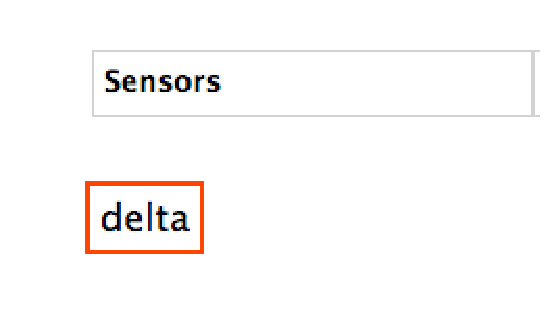
\includegraphics[width=50mm]{image/image1-1.eps}}
    \end{center}
  \end{minipage}
  \begin{minipage}{0.5\hsize}
    \begin{center}
      \fbox{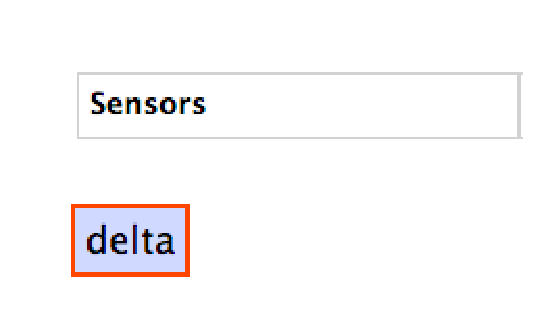
\includegraphics[width=50mm]{image/image1-2.eps}}
    \end{center}
  \end{minipage}
  \caption{点滅でのデータの通知}
  \label{fig:image01}
\end{figure}


そして二つ目として、実際の詳しいデータを見られるようにした。センサーオブジェクトに対してマウスオーバーしてフォーカスすることで実際の数字を表示できるようにした。(図\ref{fig:image02})

\begin{figure}[htbp]
    \begin{center}
       \fbox{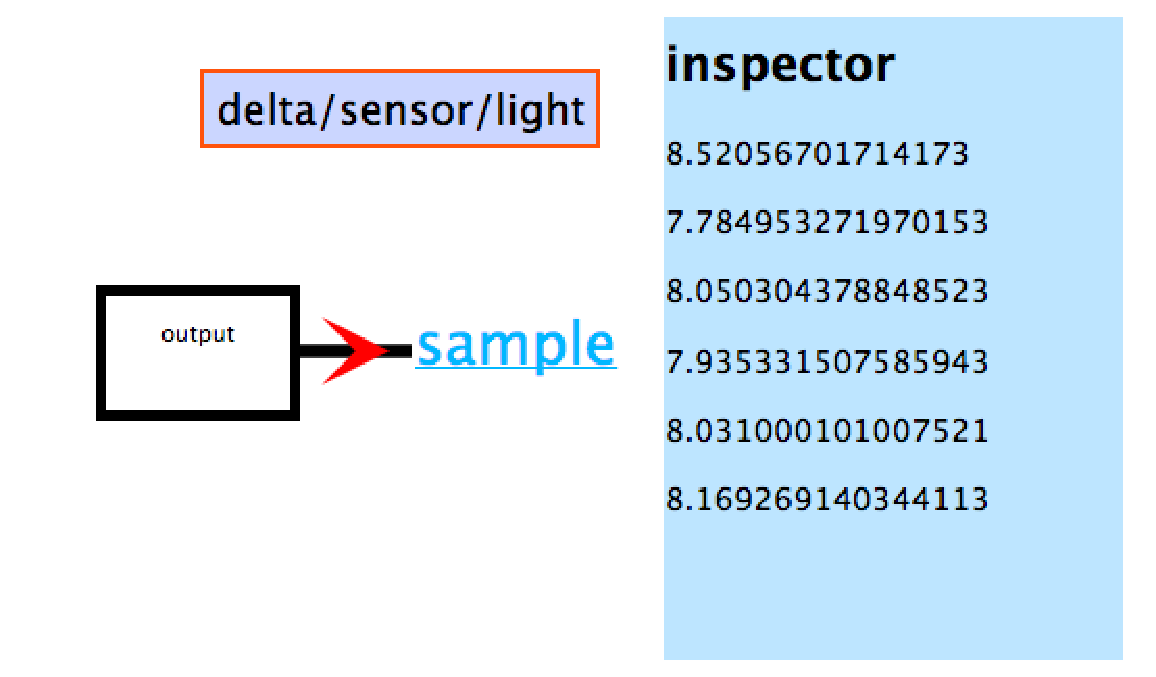
\includegraphics[width=100mm]{image/image02.eps}}
    \end{center}
    \caption{マウスオーバーによるデータの表示}
    \label{fig:image02}
\end{figure}

これら二つの実装により、センシングデータを閲覧する際に自分の欲しい粒度で取得することができるようになった。最低限の実装であれば詳しいデータが見られるだけでもいいが、抽象度を下げて色のみで表現することで閲覧する際の労力を下げることができる。

\section{ビジュアルプログラミング}

ビジュアルプログラミングを実装する際にブロック型のオブジェクトを作成した。以下にオブジェクトごとの解説をする。

\subsection{センサーオブジェクト}

ビジュアルプログラミングをする際には一番最初にセンサーオブジェクトを用意する。このオブジェクトはLindaからのデータを受信し、クライアント側でイベントを作成しデータを受信したら送信するというハブになっている。
また先に述べた通り、センサーデータが来るとこのブロックの点滅、あるいは能動的なデータの取得をすることが可能だ。

\subsection{条件オブジェクト}

センシングデータを扱うための条件オブジェクトを用意した。これにより上限下限、オンオフなどの条件分岐ができる。用意したオブジェクトを以下に列挙する。(図{\ref{fig:max}}〜図{\ref{fig:switch})これらのオブジェクトもブロックとして表現し、条件にマッチするとセンシングデータと同じように点滅する。

\begin{figure}[htbp]
  \begin{minipage}{0.5\hsize}
    \begin{center}
      \fbox{\includegraphics[width=50mm]{image/max.eps}}
    \end{center}
    \caption{Max: 最大値を設定}
    \label{fig:max}
  \end{minipage}
  \begin{minipage}{0.5\hsize}
    \begin{center}
      \fbox{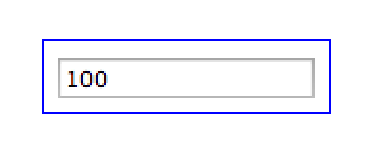
\includegraphics[width=50mm]{image/min.eps}}
    \end{center}
    \caption{min: 最小値を設定}
    \label{fig:min}
  \end{minipage}
\end{figure}

\begin{figure}[htbp]
  \begin{minipage}{0.5\hsize}
    \begin{center}
      \fbox{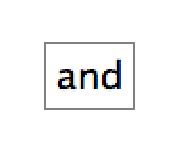
\includegraphics[width=50mm]{image/and.eps}}
    \end{center}
    \caption{and: 論理積を設定}
    \label{fig:and}
  \end{minipage}
  \begin{minipage}{0.5\hsize}
    \begin{center}
      \fbox{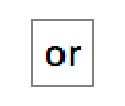
\includegraphics[width=50mm]{image/or.eps}}
    \end{center}
    \caption{or: 論理和を設定}
    \label{fig:or}
  \end{minipage}
\end{figure}

\begin{figure}[htbp]
  \begin{minipage}{0.5\hsize}
    \begin{center}
      \fbox{\includegraphics[width=50mm]{image/switch.eps}}
    \end{center}
    \caption{Switch: on/offを設定}
    \label{fig:switch}
  \end{minipage}
\end{figure}

\subsection{コネクションオブジェクト}

条件オブジェクトと同じ場所にあるが、その中で特殊なオブジェクトがコネクションオブジェクトである。コネクションオブジェクトはブロック間に親子件関係を作成できるオブジェクトである。

コネクションオブジェクトによって親のセンサーデータを条件オブジェクトの持つ自らの条件にかけ、次の世代に受け継ぐということが簡単にプログラムできるようになっている。

例えばdelta/sensor/lightからのセンサーデータかiota/sensor/lightからのセンサーデータがそれぞれ最大値10(10以下)でない場合にsampleというオブジェクトに通知を送るというような設定が簡単にできる。(図{\ref{fig:image03})

\begin{figure}[htbp]
    \begin{center}
       \fbox{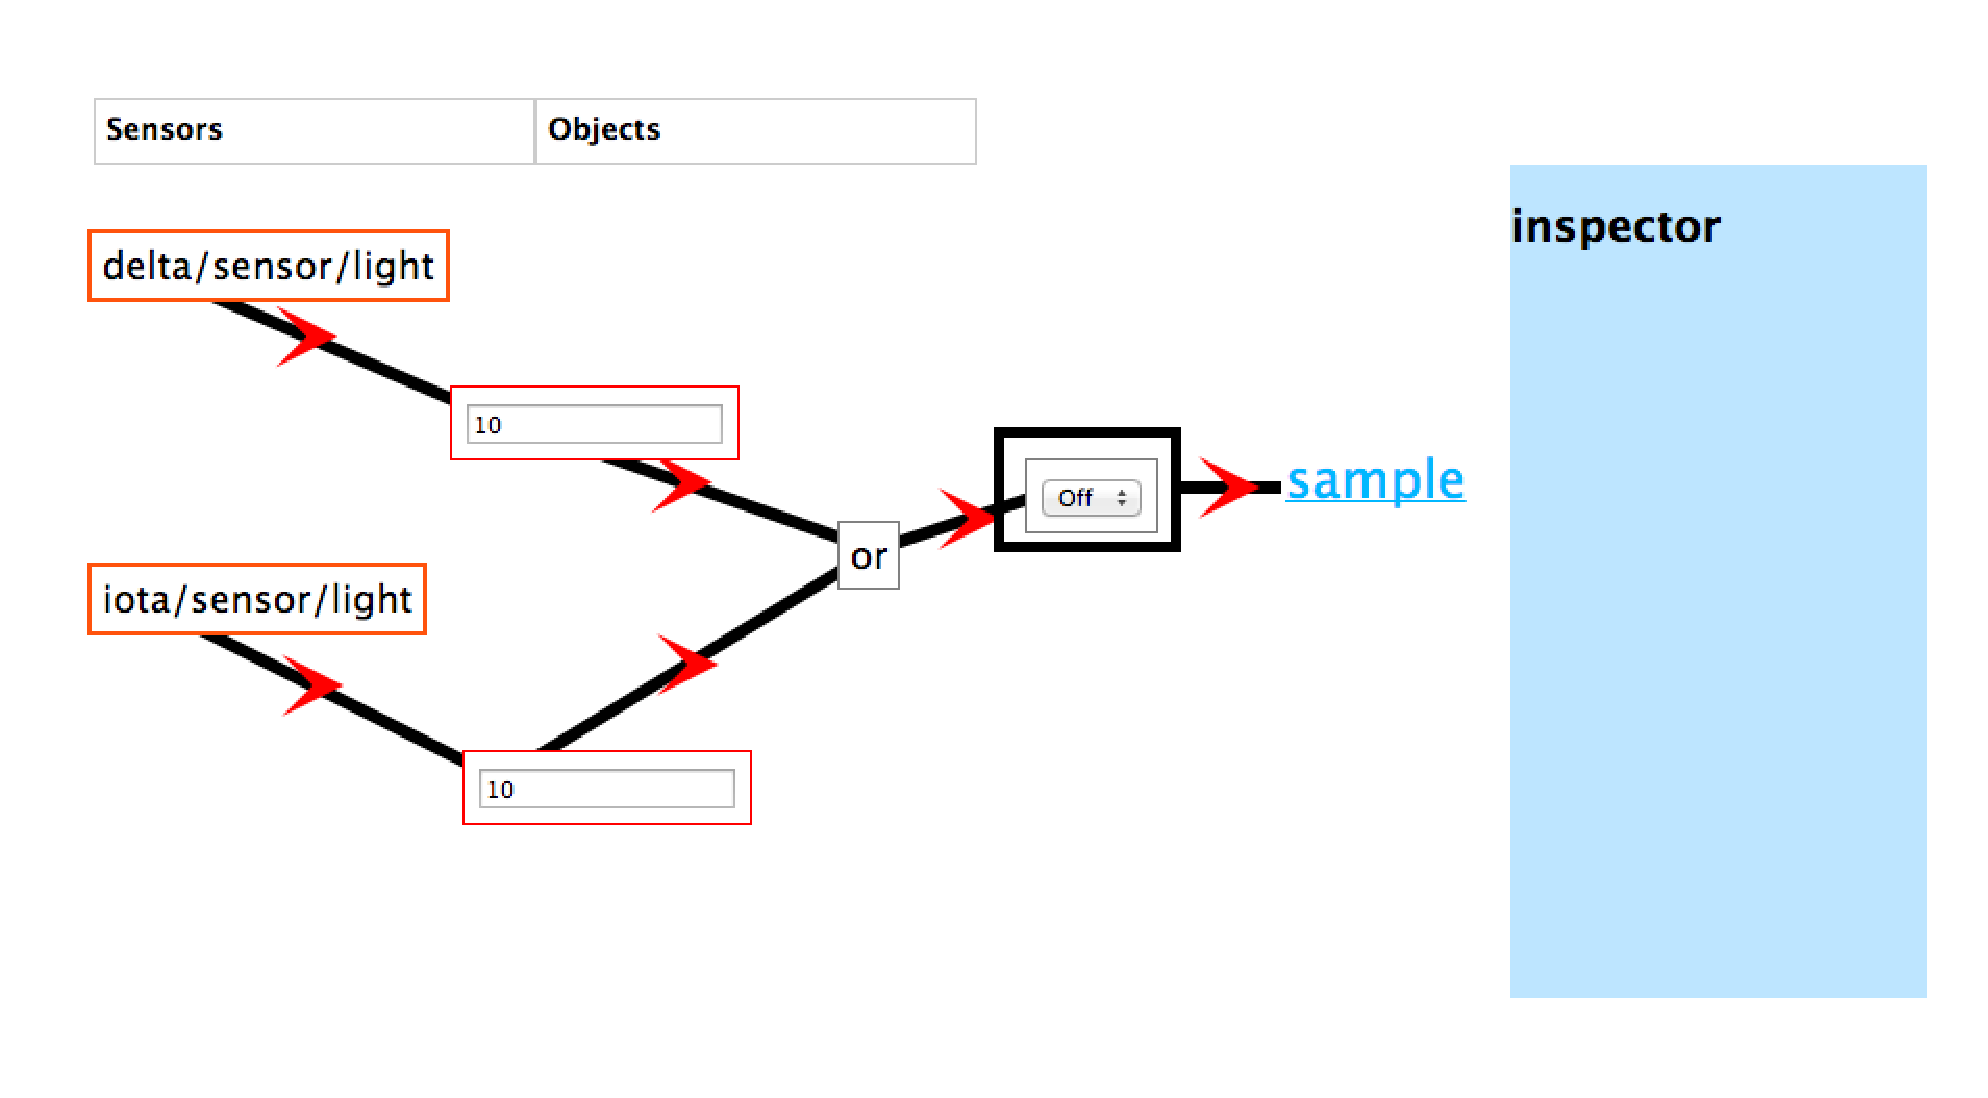
\includegraphics[width=150mm]{image/image03.eps}}
    \end{center}
    \caption{実際にセンシングデータをプログラミングする例}
    \label{fig:image03}
\end{figure}


\subsection{論文情報の設定}
\label{sec:meta}

\begin{itembox}[l]{{\tt main.tex}}
\begin{verbatim}
% 日本語情報(必要なら)
\jclass  {修士論文}                             % 論文種別
\jtitle    {修士論文用 \LaTeX\ テンプレート}    % タイトル。改行する場合は\\を入れる
\juniv    {慶應義塾大学大学院}                  % 大学名
\jfaculty  {政策・メディア研究科}               % 学部、学科
\jauthor  {ほげ山 ふう助}                       % 著者
\jhyear  {24}                                   % 平成○年度
\jsyear  {2012}                                 % 西暦○年度
\jkeyword  {\LaTeX、テンプレート、修士論文}     % 論文のキーワード
\jproject{インタラクションデザインプロジェクト} %プロジェクト名
\jdate{2013年1月}

% 英語情報(必要なら)
\eclass  {Master's Thesis}                            % 論文種別
\etitle    {A \LaTeX Template for Master Thesis}      % タイトル。改行する場合は\\を入れる
\euniv  {Keio University}                             % 大学名
\efaculty  {Graduate School of Media and Governance}  % 学部、学科
\eauthor  {Fusuke Hogeyama}                           % 著者
\eyear  {2012}                                        % 西暦○年度
\ekeyword  {\LaTeX, Templete, Master Thesis}          % 論文のキーワード
\eproject{Interaction Design Project}                 %プロジェクト名
\edate{January 2013}
\end{verbatim}
\end{itembox}

ここでは論文のタイトルや著者の氏名などのメタデータを記述する。ここで書いたデータは、表紙とアブストラクトのページに使われる。必ずしも日本語と英語の両方を設定しなければいけないわけではなくて、自分が必要とする方だけ記述すればよい。

タイトルが長過ぎる場合は、表紙やアブストラクトのページでは自動で折り返して出力される。もし改行位置を自分で指定したい場合は、その場所に \verb|\\| を入力する。


\section{出力}

\verb|\begin{document}| から \verb|\end{document}| に記述した部分が、実際に{\tt DVI}(最終的には{\tt PDF})ファイルとして出力される。

\subsection{外部ファイルの読み込み({\tt include})}

出力部分の具体的な説明の前に、外部ファイルを読み込む方法を説明する。

\verb|\begin{document}| から \verb|\end{document}| の間では、\verb|\include| コマンドを使うことで、別の {\tt *.tex} ファイルを読み込ませられる。

\begin{itembox}[l]{{\tt include}しない場合}
\begin{itembox}[l]{{\tt main.tex}}
\begin{verbatim}
\begin{document}
  \begin{jabstract}
  ほげほげ
  \end{jabstract}
\end{document}
\end{verbatim}
\end{itembox}
\end{itembox}

\begin{itembox}[l]{{\tt include}する場合}
\begin{minipage}{0.5\hsize}
\begin{itembox}[l]{{\tt main.tex}}
\begin{verbatim}
\begin{document}
\chapter{序論}
\label{chap:introduction}
\section{背景}
近年、データのセンシングが簡単になり多くのセンシングデータがビッグデータとしてあふれている。iPhoneやAndroidなどのスマートフォン端末でも位置情報や加速度、傾きなどのデータを常にセンシングすることが出来る。それに伴い、これらのセンシングデータを利用したアプリケーションが出されたり、研究目的として利用されたりするようになった。

しかしながら、これらのセンサーデータを簡単に利用できるようなフレームワークが現状存在しておらずデータをとっても活用せずに終わりといったケースが多かった。使い捨てのデータになっているこれらのデータを活用しない手はないだろう。

また、センサーデータを利用するアプリケーションは多数存在するが、個人がそれらのデータを使っているシーンは少ない。これは個人利用のハードルが高いためだ。多くの場合、プログラミング手段を用いてセンシングデータにアクセスしている。

まずはセンシングデータを可視化することでエンドユーザーに知らせることが必要だ。次点としてセンシングデータを簡単に利用できるように支援する必要がある。

個人が簡単にセンシングデータを利用できるようにするだけでより便利な世の中になるのではないだろうか。

\section{目的}
世の中に氾濫しているセンシングによるビッグデータをより効果的に利用するためのフレームワークを作成する。

そのためにまずはセンシングデータを理解できる数値、文字に変換することが必要になってくる。可視化できていなければどんなデータが利用できるかわからないためだ。

センシングデータを利用するためのフレームワークを作成する。これまでプログラミングができないとセンシングデータを利用できないケースが多くあり課題だったため、プログラミングをせずに使える直感的で使いやすいインタフェースを目指した。GUIでの操作は[1]の研究にもあるようにプログラミングせずに操作する有用な手法であると考えた。

また、他人が作ったセンシングデータをさらに再利用して使えるような仕組み作りをし、汎用的に多くの場面で使えるように想定した。

\section{本文書の構成}
第\ref{chap:introduction}章では本研究の概要を書いた。

第\ref{chap:contents}章では研究内容を説明する。第\ref{chap:prototype}章ではプロトタイプの実装方法を解説する。第\ref{chap:consideration}章では考察を書く。最後に第\ref{chap:conclusion}章にて結論を書き本論文をしめることとする。添付として参考文献を追記する。
 % 01.texをinclude
\end{document}
\end{verbatim}
\end{itembox}
\end{minipage}
\begin{minipage}{0.5\hsize}
\begin{itembox}[l]{{\tt 01.tex}}
\begin{verbatim}
\begin{jabstract}
ほげほげ
\end{jabstract}
\end{verbatim}
\end{itembox}
\end{minipage}
\end{itembox}

{\tt include}しない場合とする場合を比較するとこのとおり。どちらも出力結果は一緒。{\tt include}する場合は、読み込ませたい箇所に、読み込ませたい{\tt *.tex}ファイルの名前を、拡張子を除いて \verb|\include| コマンドで書けばよい。

\verb|\include| コマンドを用いるか用いないかは、たぶん文書量や個人の好みに依る。例えば章ごとに別のファイルにしておけば、修正箇所を探すときの手間が多少は省けるかもしれない。Gitで人と共有しつつ校正を頼むときにもファイルが分かれていたほうがコンフリクトを起こしにくい。


\subsection{表紙の出力}

\begin{itembox}[l]{{\tt main.tex}}
\begin{verbatim}
\ifjapanese
  \jmaketitle    % 表紙(日本語)
\else
  \emaketitle    % 表紙(英語)
\fi
\end{verbatim}
\end{itembox}

最初に、表紙を出力する。

\verb|\jmaketitle| が実行されると日本語の表紙が、\verb|\emaketitle| が実行されると英語の表紙がそれぞれ出力される。日本語の表紙には、第\ref{sec:meta}節で設定したうちの日本語の情報が、英語の表紙には同節で設定したうち英語の情報が、それぞれ参照されて、表記される。

デフォルトでは第\ref{sec:lang}説で設定した言語の表紙のみが出力されるようになっている。

\subsection{アブストラクトの出力}

\begin{itembox}[l]{{\tt main.tex}}
\begin{verbatim}
% ■ アブストラクトの出力 ■
%	◆書式:
%		begin{jabstract}〜end{jabstract}	:日本語のアブストラクト
%		begin{eabstract}〜end{eabstract}	:英語のアブストラクト
%		※ 不要ならばコマンドごと消せば出力されない。



% 日本語のアブストラクト
\begin{jabstract}
  近年、高性能のセンサーと豊富なリソースにより、iPhoneなどの端末で個人でも簡単にセンシングデータを取得できるようになった。加速度、傾き、位置情報など、多くのデータがビッグデータとしてあふれている。多くのデータはそれぞれが価値を持っているがそれらのデータを簡単に利用するフレームワークが現段階では存在しない。
そこで本研究ではセンシングデータを可視化し、データを簡単に取り出して利用できるフレームワークを作成した。本研究ではLindaという分散型プログラミングができるフレーワークを拡張した形になっている。Lindaは様々な場所で様々なユーザーが取得したセンシングデータをWeb上に流し、誰でも共有して利用できるようにしている。それらのセンシングデータをより簡単に利用できるようにすることで多くのプロダクトが産まれる可能性が広がるだろう。
  また、本研究ではセンシングデータを物に結びつけてプッシュAPI化する実装となっている。センシングデータを物と結びつけることでよりモジュール化し、より直感的に再利用できるメリットがある。

\end{jabstract}



% 英語のアブストラクト
	% アブストラクト。要独自コマンド、include先参照のこと
\end{verbatim}
\end{itembox}

表紙の次は、アブストラクト。

アブストラクトを出力するには、出力したい位置に、指定のコマンドを用いて文章を書き下せばよい。{\tt main.tex}に直接書いてもよいし、先述した \verb|\include| コマンドを利用して{\tt include}してもよい。

\verb|\begin{jabstract}| から \verb|\end{jabstract}| の間に書いた文章が日本語のアブストラクトとして、\verb|\begin{eabstract}| から \verb|\end{eabstract}| の間に書いた文章が英語のアブストラクトとして、それぞれ独立したページに出力される。

アブストラクトのページには、論文のタイトルやキーワードなどが、第\ref{sec:meta}節で設定した情報をもとにして自動で表記される。

日本語か英語のどちらか一方のみでよい場合は、不要な言語の方のコマンドを削除すればよい。これは、\verb|\begin| と \verb|\end| というコマンド自身も含めて削除する、ということで、\verb|\begin| と \verb|\end| の間を空っぽにするという意味ではないので注意。



\subsection{目次類の出力}
\label{sec:toc}

\begin{itembox}[l]{{\tt main.tex}}
\begin{verbatim}
\tableofcontents	% 目次
\listoffigures		% 表目次
\listoftables		% 図目次
\end{verbatim}
\end{itembox}

アブストラクトの次に、目次。文書の目次、図の目次、表の目次の三種類。

目次類を出力するには、出力したい位置に指定のコマンドを書けばよい。

これらのコマンドは、コンパイル時点での一時ファイル\footnote{{\tt *.toc}、{\tt *.lof}、{\tt *.lot}}の情報を、目次として体裁を整えて出力するもの。一時ファイルは、\verb|\begin{document}| から \verb|\end{document}| の間の章や節、図や表をコンパイルするときに、ついでに情報を取得しておいて生成される。

つまり気をつけなければいけないのは、コンパイルを一回しただけでは、一時ファイルが最新の状態に更新されるだけで、肝心の目次は正しい情報では出力されないということ。目次類を正しい情報で出力するには、最低二回のコンパイルが必要。一回目のコンパイルで一時ファイルが最新の情報に更新されて、二回目のコンパイルで初めて、その最新の一時ファイルの情報をもとに目次が出力される。

だから、文書に何らかの修正をして保存したあとは、最低でも二回、連続してコンパイルしないといけないことに注意する。

図や表を一つも使用していない場合は、目次名のみが書かれた空白のページが出力される。もしこれが不要な場合は、該当するコマンドをコメントアウトすればよい。


\subsection{本文の出力}

\begin{itembox}[l]{{\tt main.tex}}
\begin{verbatim}
\chapter{序論}
\label{chap:introduction}
\section{背景}
近年、データのセンシングが簡単になり多くのセンシングデータがビッグデータとしてあふれている。iPhoneやAndroidなどのスマートフォン端末でも位置情報や加速度、傾きなどのデータを常にセンシングすることが出来る。それに伴い、これらのセンシングデータを利用したアプリケーションが出されたり、研究目的として利用されたりするようになった。

しかしながら、これらのセンサーデータを簡単に利用できるようなフレームワークが現状存在しておらずデータをとっても活用せずに終わりといったケースが多かった。使い捨てのデータになっているこれらのデータを活用しない手はないだろう。

また、センサーデータを利用するアプリケーションは多数存在するが、個人がそれらのデータを使っているシーンは少ない。これは個人利用のハードルが高いためだ。多くの場合、プログラミング手段を用いてセンシングデータにアクセスしている。

まずはセンシングデータを可視化することでエンドユーザーに知らせることが必要だ。次点としてセンシングデータを簡単に利用できるように支援する必要がある。

個人が簡単にセンシングデータを利用できるようにするだけでより便利な世の中になるのではないだろうか。

\section{目的}
世の中に氾濫しているセンシングによるビッグデータをより効果的に利用するためのフレームワークを作成する。

そのためにまずはセンシングデータを理解できる数値、文字に変換することが必要になってくる。可視化できていなければどんなデータが利用できるかわからないためだ。

センシングデータを利用するためのフレームワークを作成する。これまでプログラミングができないとセンシングデータを利用できないケースが多くあり課題だったため、プログラミングをせずに使える直感的で使いやすいインタフェースを目指した。GUIでの操作は[1]の研究にもあるようにプログラミングせずに操作する有用な手法であると考えた。

また、他人が作ったセンシングデータをさらに再利用して使えるような仕組み作りをし、汎用的に多くの場面で使えるように想定した。

\section{本文書の構成}
第\ref{chap:introduction}章では本研究の概要を書いた。

第\ref{chap:contents}章では研究内容を説明する。第\ref{chap:prototype}章ではプロトタイプの実装方法を解説する。第\ref{chap:consideration}章では考察を書く。最後に第\ref{chap:conclusion}章にて結論を書き本論文をしめることとする。添付として参考文献を追記する。
	% 本文1
\chapter{研究内容}
\label{chap:contents}

本章では、本研究の内容を説明する。

\section{システム概要}

本システムはセンシングデータを個人でも簡単に利用できるようにすることが目的だ。
そのためのフレームワークを作成し、センシングデータを可視化するという二つの軸をもってシステムを構成した。

以下にシステムの構成を示す。大枠として、Linda\footnote{データをクラウド上で共有するためのフレームワーク。並列処理をしており、同時に多くのクライアントを処理できる。}からサーバーがデータを取得し、クライアントのリクエストに応じて送信する。クライアントでの情報は随時データベースに保存する。

\begin{table}[htbp]
  \caption{システム構成}
  \label{tb:files}
  \begin{center}\begin{tabular}{c|l}
    \hline
    システム&概要\\\hline\hline
    {\tt Linda}&データ元。データストリームからデータを取得する。\\\hline
    {\tt サーバー}&Lindaからデータを取得し、クライアントからのリクエストが来たら送信する。\\\hline
    {\tt クライアント}&サーバーにデータを要求し、ビジュアルプログラミングのビューを提供する。\\\hline
    {\tt データベース}&サーバー、クライアントのデータを保存している。\\\hline
  \end{tabular}\end{center}
\end{table}

\section{データの可視化}
センサーデータを二つの方法で可視化した。

まず一つ目として点滅によるデータの受信だ。Lindaから送られてきたデータを受信するとブロックが青に変化し、元に戻る。(図\ref{fig:image01})
センシングデータを監視してすぐにデータの受信に気付くことができるというメリットがある。\\

\begin{figure}[htbp]
  \begin{minipage}{0.5\hsize}
    \begin{center}
      \fbox{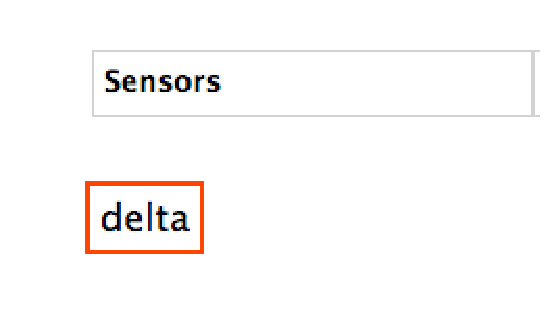
\includegraphics[width=50mm]{image/image1-1.eps}}
    \end{center}
  \end{minipage}
  \begin{minipage}{0.5\hsize}
    \begin{center}
      \fbox{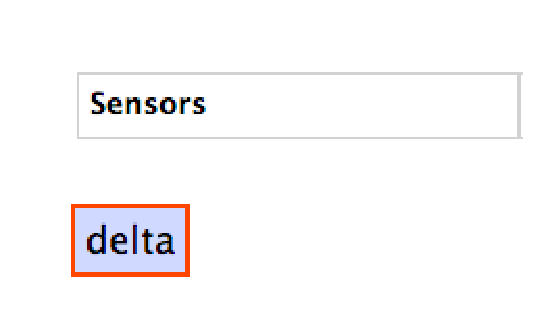
\includegraphics[width=50mm]{image/image1-2.eps}}
    \end{center}
  \end{minipage}
  \caption{点滅でのデータの通知}
  \label{fig:image01}
\end{figure}


そして二つ目として、実際の詳しいデータを見られるようにした。センサーオブジェクトに対してマウスオーバーしてフォーカスすることで実際の数字を表示できるようにした。(図\ref{fig:image02})

\begin{figure}[htbp]
    \begin{center}
       \fbox{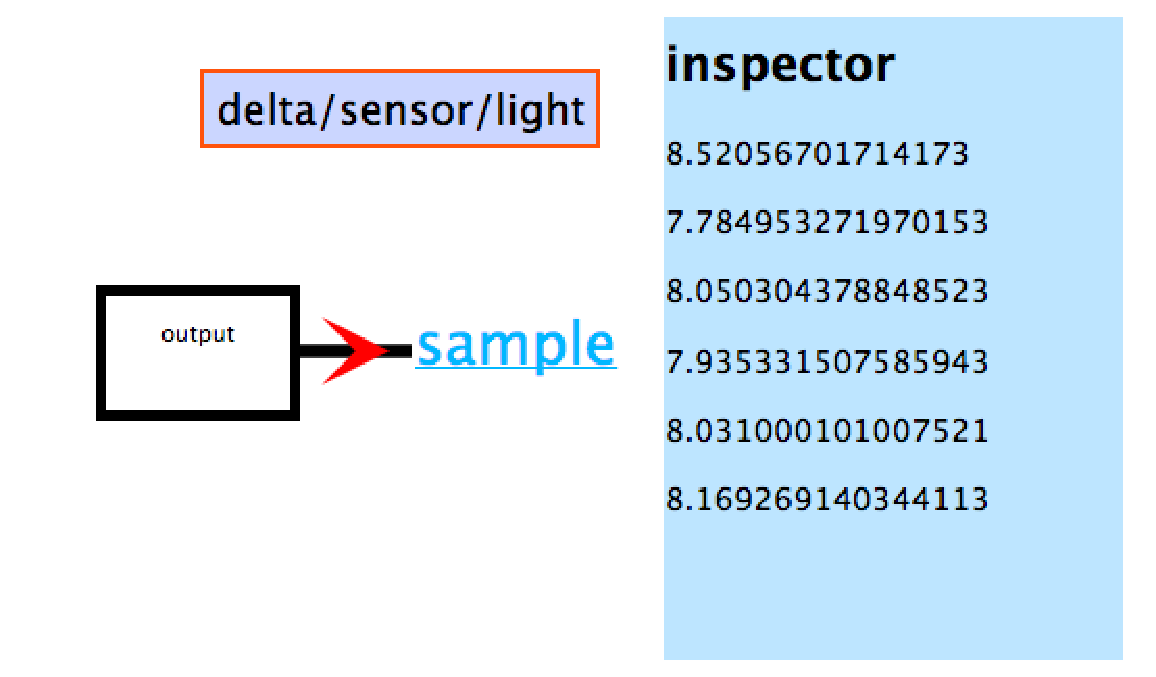
\includegraphics[width=100mm]{image/image02.eps}}
    \end{center}
    \caption{マウスオーバーによるデータの表示}
    \label{fig:image02}
\end{figure}

これら二つの実装により、センシングデータを閲覧する際に自分の欲しい粒度で取得することができるようになった。最低限の実装であれば詳しいデータが見られるだけでもいいが、抽象度を下げて色のみで表現することで閲覧する際の労力を下げることができる。

\section{ビジュアルプログラミング}

ビジュアルプログラミングを実装する際にブロック型のオブジェクトを作成した。以下にオブジェクトごとの解説をする。

\subsection{センサーオブジェクト}

ビジュアルプログラミングをする際には一番最初にセンサーオブジェクトを用意する。このオブジェクトはLindaからのデータを受信し、クライアント側でイベントを作成しデータを受信したら送信するというハブになっている。
また先に述べた通り、センサーデータが来るとこのブロックの点滅、あるいは能動的なデータの取得をすることが可能だ。

\subsection{条件オブジェクト}

センシングデータを扱うための条件オブジェクトを用意した。これにより上限下限、オンオフなどの条件分岐ができる。用意したオブジェクトを以下に列挙する。(図{\ref{fig:max}}〜図{\ref{fig:switch})これらのオブジェクトもブロックとして表現し、条件にマッチするとセンシングデータと同じように点滅する。

\begin{figure}[htbp]
  \begin{minipage}{0.5\hsize}
    \begin{center}
      \fbox{\includegraphics[width=50mm]{image/max.eps}}
    \end{center}
    \caption{Max: 最大値を設定}
    \label{fig:max}
  \end{minipage}
  \begin{minipage}{0.5\hsize}
    \begin{center}
      \fbox{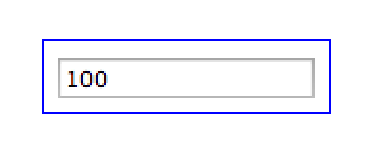
\includegraphics[width=50mm]{image/min.eps}}
    \end{center}
    \caption{min: 最小値を設定}
    \label{fig:min}
  \end{minipage}
\end{figure}

\begin{figure}[htbp]
  \begin{minipage}{0.5\hsize}
    \begin{center}
      \fbox{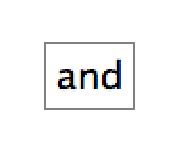
\includegraphics[width=50mm]{image/and.eps}}
    \end{center}
    \caption{and: 論理積を設定}
    \label{fig:and}
  \end{minipage}
  \begin{minipage}{0.5\hsize}
    \begin{center}
      \fbox{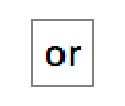
\includegraphics[width=50mm]{image/or.eps}}
    \end{center}
    \caption{or: 論理和を設定}
    \label{fig:or}
  \end{minipage}
\end{figure}

\begin{figure}[htbp]
  \begin{minipage}{0.5\hsize}
    \begin{center}
      \fbox{\includegraphics[width=50mm]{image/switch.eps}}
    \end{center}
    \caption{Switch: on/offを設定}
    \label{fig:switch}
  \end{minipage}
\end{figure}

\subsection{コネクションオブジェクト}

条件オブジェクトと同じ場所にあるが、その中で特殊なオブジェクトがコネクションオブジェクトである。コネクションオブジェクトはブロック間に親子件関係を作成できるオブジェクトである。

コネクションオブジェクトによって親のセンサーデータを条件オブジェクトの持つ自らの条件にかけ、次の世代に受け継ぐということが簡単にプログラムできるようになっている。

例えばdelta/sensor/lightからのセンサーデータかiota/sensor/lightからのセンサーデータがそれぞれ最大値10(10以下)でない場合にsampleというオブジェクトに通知を送るというような設定が簡単にできる。(図{\ref{fig:image03})

\begin{figure}[htbp]
    \begin{center}
       \fbox{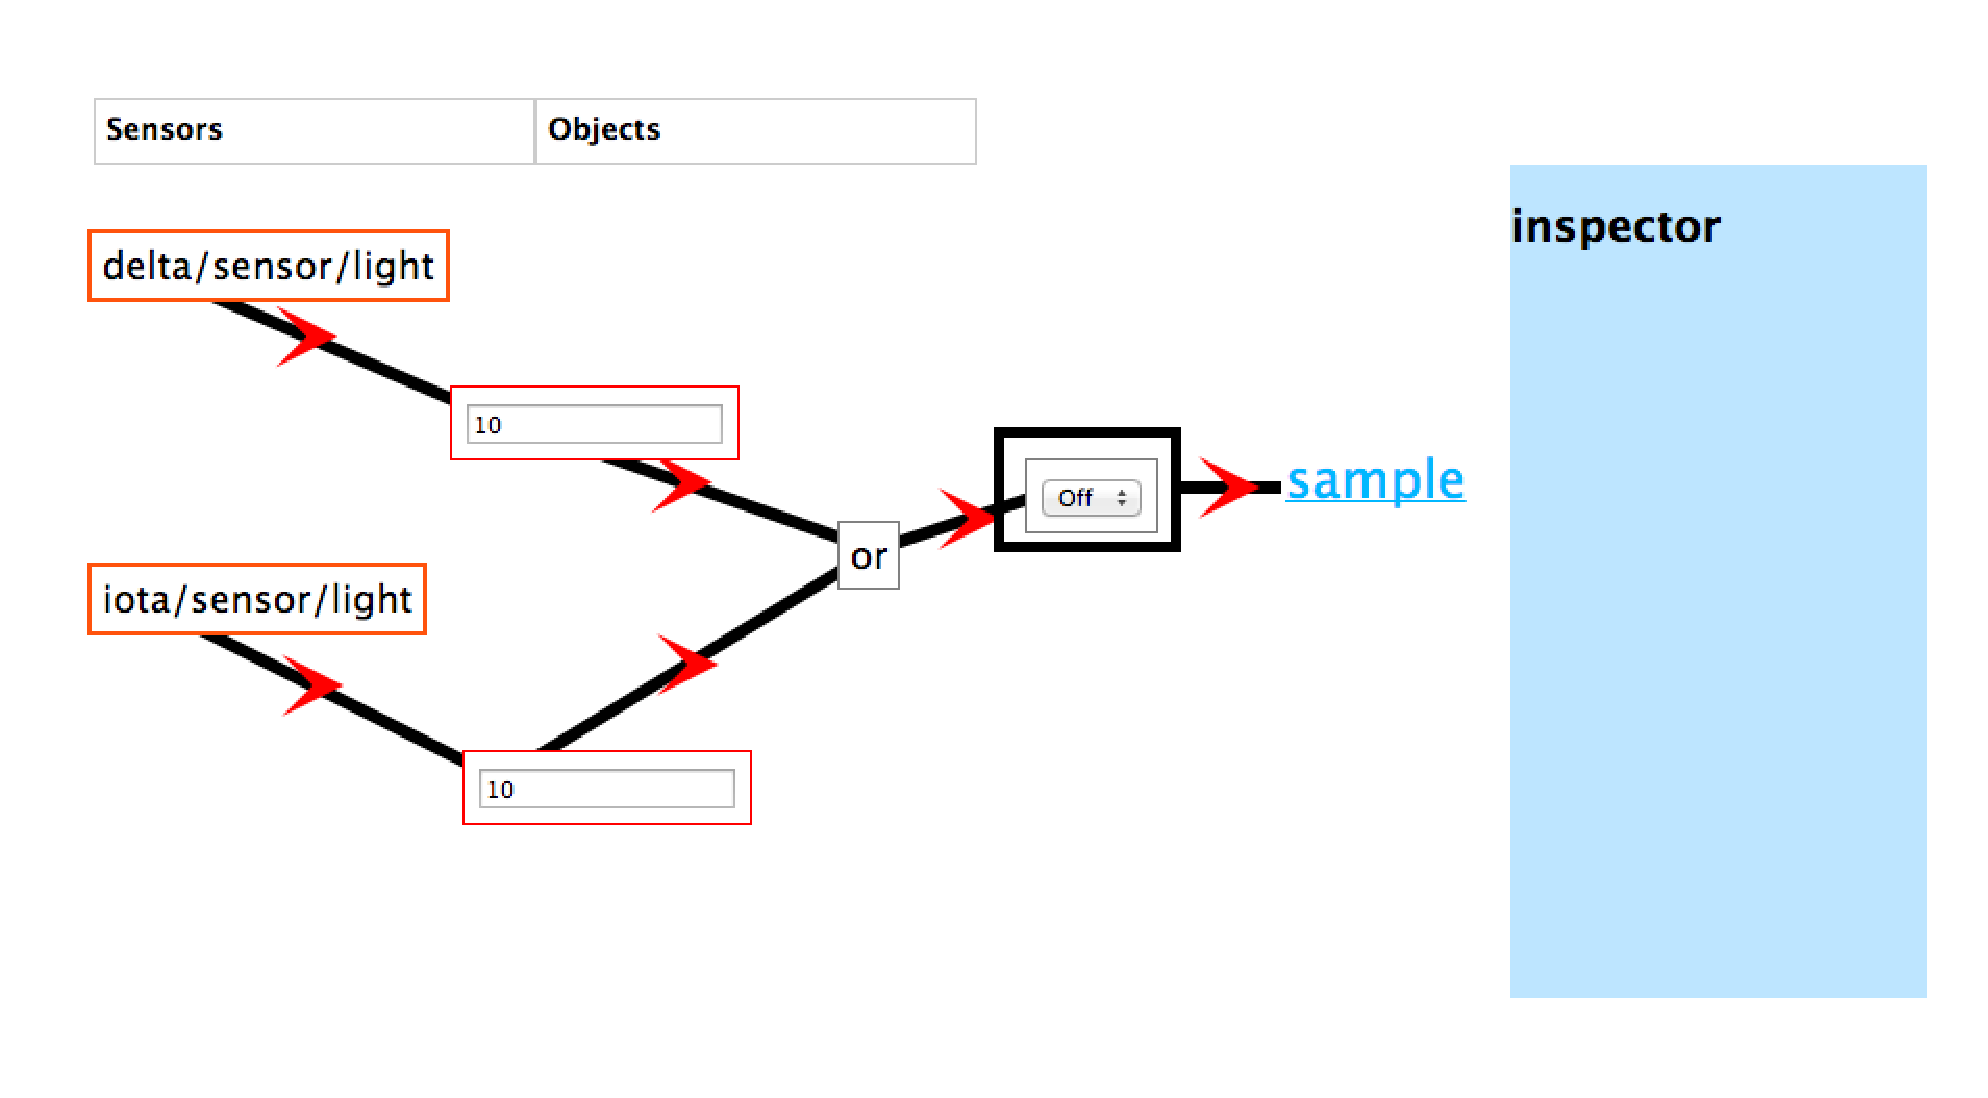
\includegraphics[width=150mm]{image/image03.eps}}
    \end{center}
    \caption{実際にセンシングデータをプログラミングする例}
    \label{fig:image03}
\end{figure}


\subsection{論文情報の設定}
\label{sec:meta}

\begin{itembox}[l]{{\tt main.tex}}
\begin{verbatim}
% 日本語情報(必要なら)
\jclass  {修士論文}                             % 論文種別
\jtitle    {修士論文用 \LaTeX\ テンプレート}    % タイトル。改行する場合は\\を入れる
\juniv    {慶應義塾大学大学院}                  % 大学名
\jfaculty  {政策・メディア研究科}               % 学部、学科
\jauthor  {ほげ山 ふう助}                       % 著者
\jhyear  {24}                                   % 平成○年度
\jsyear  {2012}                                 % 西暦○年度
\jkeyword  {\LaTeX、テンプレート、修士論文}     % 論文のキーワード
\jproject{インタラクションデザインプロジェクト} %プロジェクト名
\jdate{2013年1月}

% 英語情報(必要なら)
\eclass  {Master's Thesis}                            % 論文種別
\etitle    {A \LaTeX Template for Master Thesis}      % タイトル。改行する場合は\\を入れる
\euniv  {Keio University}                             % 大学名
\efaculty  {Graduate School of Media and Governance}  % 学部、学科
\eauthor  {Fusuke Hogeyama}                           % 著者
\eyear  {2012}                                        % 西暦○年度
\ekeyword  {\LaTeX, Templete, Master Thesis}          % 論文のキーワード
\eproject{Interaction Design Project}                 %プロジェクト名
\edate{January 2013}
\end{verbatim}
\end{itembox}

ここでは論文のタイトルや著者の氏名などのメタデータを記述する。ここで書いたデータは、表紙とアブストラクトのページに使われる。必ずしも日本語と英語の両方を設定しなければいけないわけではなくて、自分が必要とする方だけ記述すればよい。

タイトルが長過ぎる場合は、表紙やアブストラクトのページでは自動で折り返して出力される。もし改行位置を自分で指定したい場合は、その場所に \verb|\\| を入力する。


\section{出力}

\verb|\begin{document}| から \verb|\end{document}| に記述した部分が、実際に{\tt DVI}(最終的には{\tt PDF})ファイルとして出力される。

\subsection{外部ファイルの読み込み({\tt include})}

出力部分の具体的な説明の前に、外部ファイルを読み込む方法を説明する。

\verb|\begin{document}| から \verb|\end{document}| の間では、\verb|\include| コマンドを使うことで、別の {\tt *.tex} ファイルを読み込ませられる。

\begin{itembox}[l]{{\tt include}しない場合}
\begin{itembox}[l]{{\tt main.tex}}
\begin{verbatim}
\begin{document}
  \begin{jabstract}
  ほげほげ
  \end{jabstract}
\end{document}
\end{verbatim}
\end{itembox}
\end{itembox}

\begin{itembox}[l]{{\tt include}する場合}
\begin{minipage}{0.5\hsize}
\begin{itembox}[l]{{\tt main.tex}}
\begin{verbatim}
\begin{document}
\include{01} % 01.texをinclude
\end{document}
\end{verbatim}
\end{itembox}
\end{minipage}
\begin{minipage}{0.5\hsize}
\begin{itembox}[l]{{\tt 01.tex}}
\begin{verbatim}
\begin{jabstract}
ほげほげ
\end{jabstract}
\end{verbatim}
\end{itembox}
\end{minipage}
\end{itembox}

{\tt include}しない場合とする場合を比較するとこのとおり。どちらも出力結果は一緒。{\tt include}する場合は、読み込ませたい箇所に、読み込ませたい{\tt *.tex}ファイルの名前を、拡張子を除いて \verb|\include| コマンドで書けばよい。

\verb|\include| コマンドを用いるか用いないかは、たぶん文書量や個人の好みに依る。例えば章ごとに別のファイルにしておけば、修正箇所を探すときの手間が多少は省けるかもしれない。Gitで人と共有しつつ校正を頼むときにもファイルが分かれていたほうがコンフリクトを起こしにくい。


\subsection{表紙の出力}

\begin{itembox}[l]{{\tt main.tex}}
\begin{verbatim}
\ifjapanese
  \jmaketitle    % 表紙(日本語)
\else
  \emaketitle    % 表紙(英語)
\fi
\end{verbatim}
\end{itembox}

最初に、表紙を出力する。

\verb|\jmaketitle| が実行されると日本語の表紙が、\verb|\emaketitle| が実行されると英語の表紙がそれぞれ出力される。日本語の表紙には、第\ref{sec:meta}節で設定したうちの日本語の情報が、英語の表紙には同節で設定したうち英語の情報が、それぞれ参照されて、表記される。

デフォルトでは第\ref{sec:lang}説で設定した言語の表紙のみが出力されるようになっている。

\subsection{アブストラクトの出力}

\begin{itembox}[l]{{\tt main.tex}}
\begin{verbatim}
\include{00_abstract}	% アブストラクト。要独自コマンド、include先参照のこと
\end{verbatim}
\end{itembox}

表紙の次は、アブストラクト。

アブストラクトを出力するには、出力したい位置に、指定のコマンドを用いて文章を書き下せばよい。{\tt main.tex}に直接書いてもよいし、先述した \verb|\include| コマンドを利用して{\tt include}してもよい。

\verb|\begin{jabstract}| から \verb|\end{jabstract}| の間に書いた文章が日本語のアブストラクトとして、\verb|\begin{eabstract}| から \verb|\end{eabstract}| の間に書いた文章が英語のアブストラクトとして、それぞれ独立したページに出力される。

アブストラクトのページには、論文のタイトルやキーワードなどが、第\ref{sec:meta}節で設定した情報をもとにして自動で表記される。

日本語か英語のどちらか一方のみでよい場合は、不要な言語の方のコマンドを削除すればよい。これは、\verb|\begin| と \verb|\end| というコマンド自身も含めて削除する、ということで、\verb|\begin| と \verb|\end| の間を空っぽにするという意味ではないので注意。



\subsection{目次類の出力}
\label{sec:toc}

\begin{itembox}[l]{{\tt main.tex}}
\begin{verbatim}
\tableofcontents	% 目次
\listoffigures		% 表目次
\listoftables		% 図目次
\end{verbatim}
\end{itembox}

アブストラクトの次に、目次。文書の目次、図の目次、表の目次の三種類。

目次類を出力するには、出力したい位置に指定のコマンドを書けばよい。

これらのコマンドは、コンパイル時点での一時ファイル\footnote{{\tt *.toc}、{\tt *.lof}、{\tt *.lot}}の情報を、目次として体裁を整えて出力するもの。一時ファイルは、\verb|\begin{document}| から \verb|\end{document}| の間の章や節、図や表をコンパイルするときに、ついでに情報を取得しておいて生成される。

つまり気をつけなければいけないのは、コンパイルを一回しただけでは、一時ファイルが最新の状態に更新されるだけで、肝心の目次は正しい情報では出力されないということ。目次類を正しい情報で出力するには、最低二回のコンパイルが必要。一回目のコンパイルで一時ファイルが最新の情報に更新されて、二回目のコンパイルで初めて、その最新の一時ファイルの情報をもとに目次が出力される。

だから、文書に何らかの修正をして保存したあとは、最低でも二回、連続してコンパイルしないといけないことに注意する。

図や表を一つも使用していない場合は、目次名のみが書かれた空白のページが出力される。もしこれが不要な場合は、該当するコマンドをコメントアウトすればよい。


\subsection{本文の出力}

\begin{itembox}[l]{{\tt main.tex}}
\begin{verbatim}
\include{01}	% 本文1
\include{02}	% 本文2
\include{03}	% 本文3
\include{04}	% 本文4
\end{verbatim}
\end{itembox}

目次に続いて、論文のメイン、本文を記述する。アブストラクトと同様で、{\tt main.tex}に直接書くか、\verb|\include| コマンドを利用して別に用意したファイルを{\tt include}する。

本文の書き方は、第\ref{chap:latex}章で詳しく説明する。


\subsection{謝辞の出力}

\begin{itembox}[l]{{\tt main.tex}}
\begin{verbatim}
\include{90_acknowledgment}	% 謝辞。要独自コマンド、include先参照のこと
\end{verbatim}
\end{itembox}

本文のあとには、謝辞を出力する。\verb|begin{acknowledgment}| から \verb|end{acknowledgment}| の間に書いた文章が、謝辞として独立したページに出力される。アブストラクトや本文と同じで、{\tt main.tex}に直接書いてもよいし、\verb|\include| コマンドを利用して{\tt include}してもよい。


\subsection{参考文献の出力}

\begin{itembox}[l]{{\tt main.tex}}
\begin{verbatim}
\include{91_bibliography}	% 参考文献。要独自コマンド、include先参照のこと
\end{verbatim}
\end{itembox}

謝辞に続いて、参考文献を出力する。

参考文献リストは、\verb|\begin{bib}| から \verb|\end{bib}| の間に、\verb|\bibitem| コマンドを使って書く。

BibTeXを使う場合は、以下のようにする。

\begin{itembox}[l]{{\tt 91\_bibliography.tex}}
\begin{verbatim}
\begin{bib}[100]
\bibliography{main}
\end{bib}
\end{verbatim}
\end{itembox}

こうすると、\verb|main.bib|から使用した参考文献のみを抽出して出力してくれる。\verb|main.bib|の中身は以下のようになっていて、気の利いた論文検索サイトであればBibTeXをコピペできるようになっているので簡単に作れるはず。


\begin{itembox}[l]{{\tt 91\_bibliography.tex}}
\begin{verbatim}
@article{hoge09,
    author  = "ほげ山太郎 and ほげ山次郎",
    yomi    = "ほげやまたろう",
    title   = "ほげほげ理論のHCI分野への応用",
    journal = "ほげほげ学会論文誌",
    volume  = "31",
    number  = "3",
    pages   = "194-201",
    year    = "2009",
}
@inproceedings{hoge08,
    author     = "Taro Hogeyama and Jiro Hogeyama",
    title      = "The Theory of Hoge",
    booktitle  = "The Proceedings of The Hoge Society",
    year       = "2008"
}
\end{verbatim}
\end{itembox}


以下は、BibTeXを使わないで手で書く例。

\begin{itembox}[l]{{\tt 91\_bibliography.tex}}
\begin{verbatim}
@article{hoge09,
    author  = "ほげ山太郎 and ほげ山次郎",
    yomi    = "ほげやまたろう",
    title   = "ほげほげ理論のHCI分野への応用",
    journal = "ほげほげ学会論文誌",
    volume  = "31",
    number  = "3",
    pages   = "194-201",
    year    = "2009",
}
@inproceedings{hoge08,
    author     = "Taro Hogeyama and Jiro Hogeyama",
    title      = "The Theory of Hoge",
    booktitle  = "The Proceedings of The Hoge Society",
    year       = "2008"
}
\end{verbatim}
\end{itembox}


英語の文献の場合、慣例的に書誌名をイタリック体にすることが多いらしい。

\begin{itembox}[l]{{\tt 91\_bibliography.tex}}
\begin{verbatim}
\begin{bib}[100]
\begin{thebibliography}{#1}
% \bibitem{参照用名称}
%   著者名:
%   \newblock 文献名,
%   \newblock 書誌情報,出版年.

\bibitem{hoge09}
  ほげ山太郎,ほげ山次郎:
  \newblock ほげほげ理論のHCI分野への応用,
  \newblock ほげほげ学会論文誌,Vol.31,No.3,pp.194-201,2009.

\bibitem{hoge08}
  Taro Hogeyama, Jiro Hogeyama:
  \newblock The Theory of Hoge,
  \newblock {\it The Proceedings of The Hoge Society}, 2008.
\end{thebibliography}
\end{bib}
\end{verbatim}
\end{itembox}

\verb|\bibitem| コマンド中、参照用名称は、本文から参考文献を参照するときに使うので、忘れずに書いておく。参照文献を本文中に参照するときには、\verb|\cite{参照用名称}| のように書けばよい。例えば、この文の末尾には \verb|\cite{hoge09}| と書いてあるので、自動で対応する番号が振られる\cite{hoge09}\cite{hoge08}。

参考文献リストの番号付けと、本文で参照したときの番号の挿入は、全部が自動で行われる。ただしこれも、第\ref{sec:toc}節で説明した目次の出力と同じで、一時ファイルを生成してからの挿入なので、正しく出力するには最低でも二回のコンパイルが必要。BibTeXを使用する場合は、\verb|platex|コマンドのあと\verb|pbibtex|コマンドを実行し、さらに2回\verb|platex|コマンドを実行するといいらしい。



\subsection{付録の出力}

\begin{itembox}[l]{{\tt main.tex}}
\begin{verbatim}
\appendix
\include{92_appendix}		% 付録
\end{verbatim}
\end{itembox}

必要であれば、論文の最後には付録を出力する。

\verb|\appendix| コマンド以降に書いたものは、すべて付録として扱われる。付録部分の書き方は通常の本文とまったく同じで、\verb|\appendix| コマンド以降に書くだけで勝手に付録用の体裁で出力される。
	% 本文2
\chapter{プロトタイプの実装}
\label{chap:prototype}

この章では本研究でのプロトタイプを実装し、その流れを解説する。

\section{実装概要}
大量のデータをやりとりすることを想定してnode.js\footnote{http://www.nodejs.org/}で実装した。またデータベースはmongoDB\footnote{http://www.mongodb.org/}を採用し、軽量フレームワークを実現した。元になっているセンサーデータはLindaを利用し、データを取得、書き込みしている。

クライアントサイドではJQuery UI\footnote{http://jqueryui.com/}とSVG\footnote{http://www.w3.org/Graphics/SVG/}を使い、ドラッグ&ドロップと線の描画を実現している。

\section{ページ遷移}
パスによってページを管理している。基本的にはパスの名前が最終的に結びつけるオブジェクトの名前になっている。パスにアクセスした際、オブジェクトが作成されていなかった場合には新しいオブジェクトの作成が促され、データベースに記録される。ユーザーはそのオブジェクトに対してアクションとその条件を指定することでプログラムしていく。/keyというページに最初にアクセスした際にはkeyオブジェクトを作成する。最終的なアクションは/key/outputでPOST送信先を設定する。例えば部屋の明るさをセンシングし、部屋が暗くなったらという条件をkeyオブジェクトに紐付け、携帯に通知を送るというアクションを実行することなどができる。その他にも鍵の開け閉めをWebで管理している場合にはそのURLにリクエストを送ることもできる。

/controlのパスはデータベースの管理ができるようになっており、センサーやオブジェクトに追加が出来るようになっている。


\section{サーバーサイド}
言語はJavascriptを使い、node.jsのsocket.io\footnote{http://socket.io/}で実装した。センサーオブジェクトに対して常にコネクションを貼り、データをemitしている。mongoDBではセンサーデータ、オブジェクトデータ、コネクションデータ、クライアントデータを保存している。

\section{クライアントサイド}
クライアントサイドもサーバーサイドと同様にJavascriptを選択した。ページ内でオブジェクトの作成、移動、コネクションの作成などのアクションが行われた際に常にサーバー側に情報を送り保存している。イベントの制御にはEvent Emitter\footnote{http://nodejs.org/api/events.html}を用いた。Event Emitterを使えばオブジェクト自体にイベントを持たせることができる。それぞれのオブジェクトが送られてきたデータを監視し、自分の持っている条件にマッチしたら自らが送信側になるという実装をしている。下の図ではdelta/sensor/lightというセンサーを親データとして、orというオブジェクトが監視して条件に照らし合わせマッチしたら発信するオブジェクトになっている。(図\ref{fig:image09})

\begin{figure}[htbp]
  \begin{center}
    \fbox{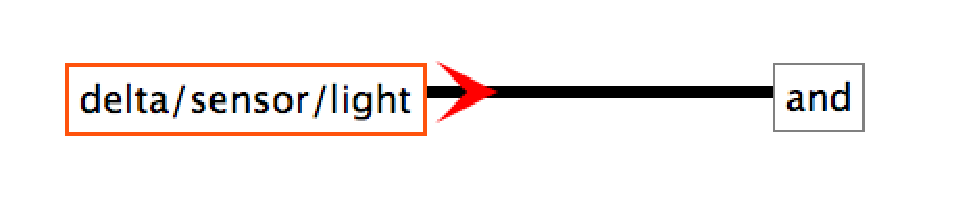
\includegraphics[width=100mm]{image/image09.eps}}
  \end{center}
  \caption{センサーデータの親子関係}
  \label{fig:image09}
\end{figure}

	% 本文3
\chapter{利用法}
\label{chap:usage}
この章ではセンシングデータの利用法を具体的に提案する。\\
センシングデータといってもWeb上で取得できる物は全てデータとして扱うことが出来る。
例えば藤沢の気温データをWeb上から更新される度に取得することで気温のセンシングデータを作成できる。また、現在時刻やPCのファイル情報などユーザーのコンテキストも取得してデータにすることが出来る。
これらのデータを使えば条件指定の幅が広がり複雑なプログラムを簡単に書くことが出来る。

\section{ニュース購読}
現在時刻を取得することで簡単にアラーム機能を実装できる。指定の時間をすぎるとニュースを取得し、PCに喋らせているのが以下の例だ。Macのsayコマンドを使って特定のPCから音声を発信している。
(図\ref{fig:image10})では時間を取得するtimeオブジェクトが9時と21時にマッチした時にnewsにアクセスしている。
\begin{figure}[htbp]
  \begin{center}
    \fbox{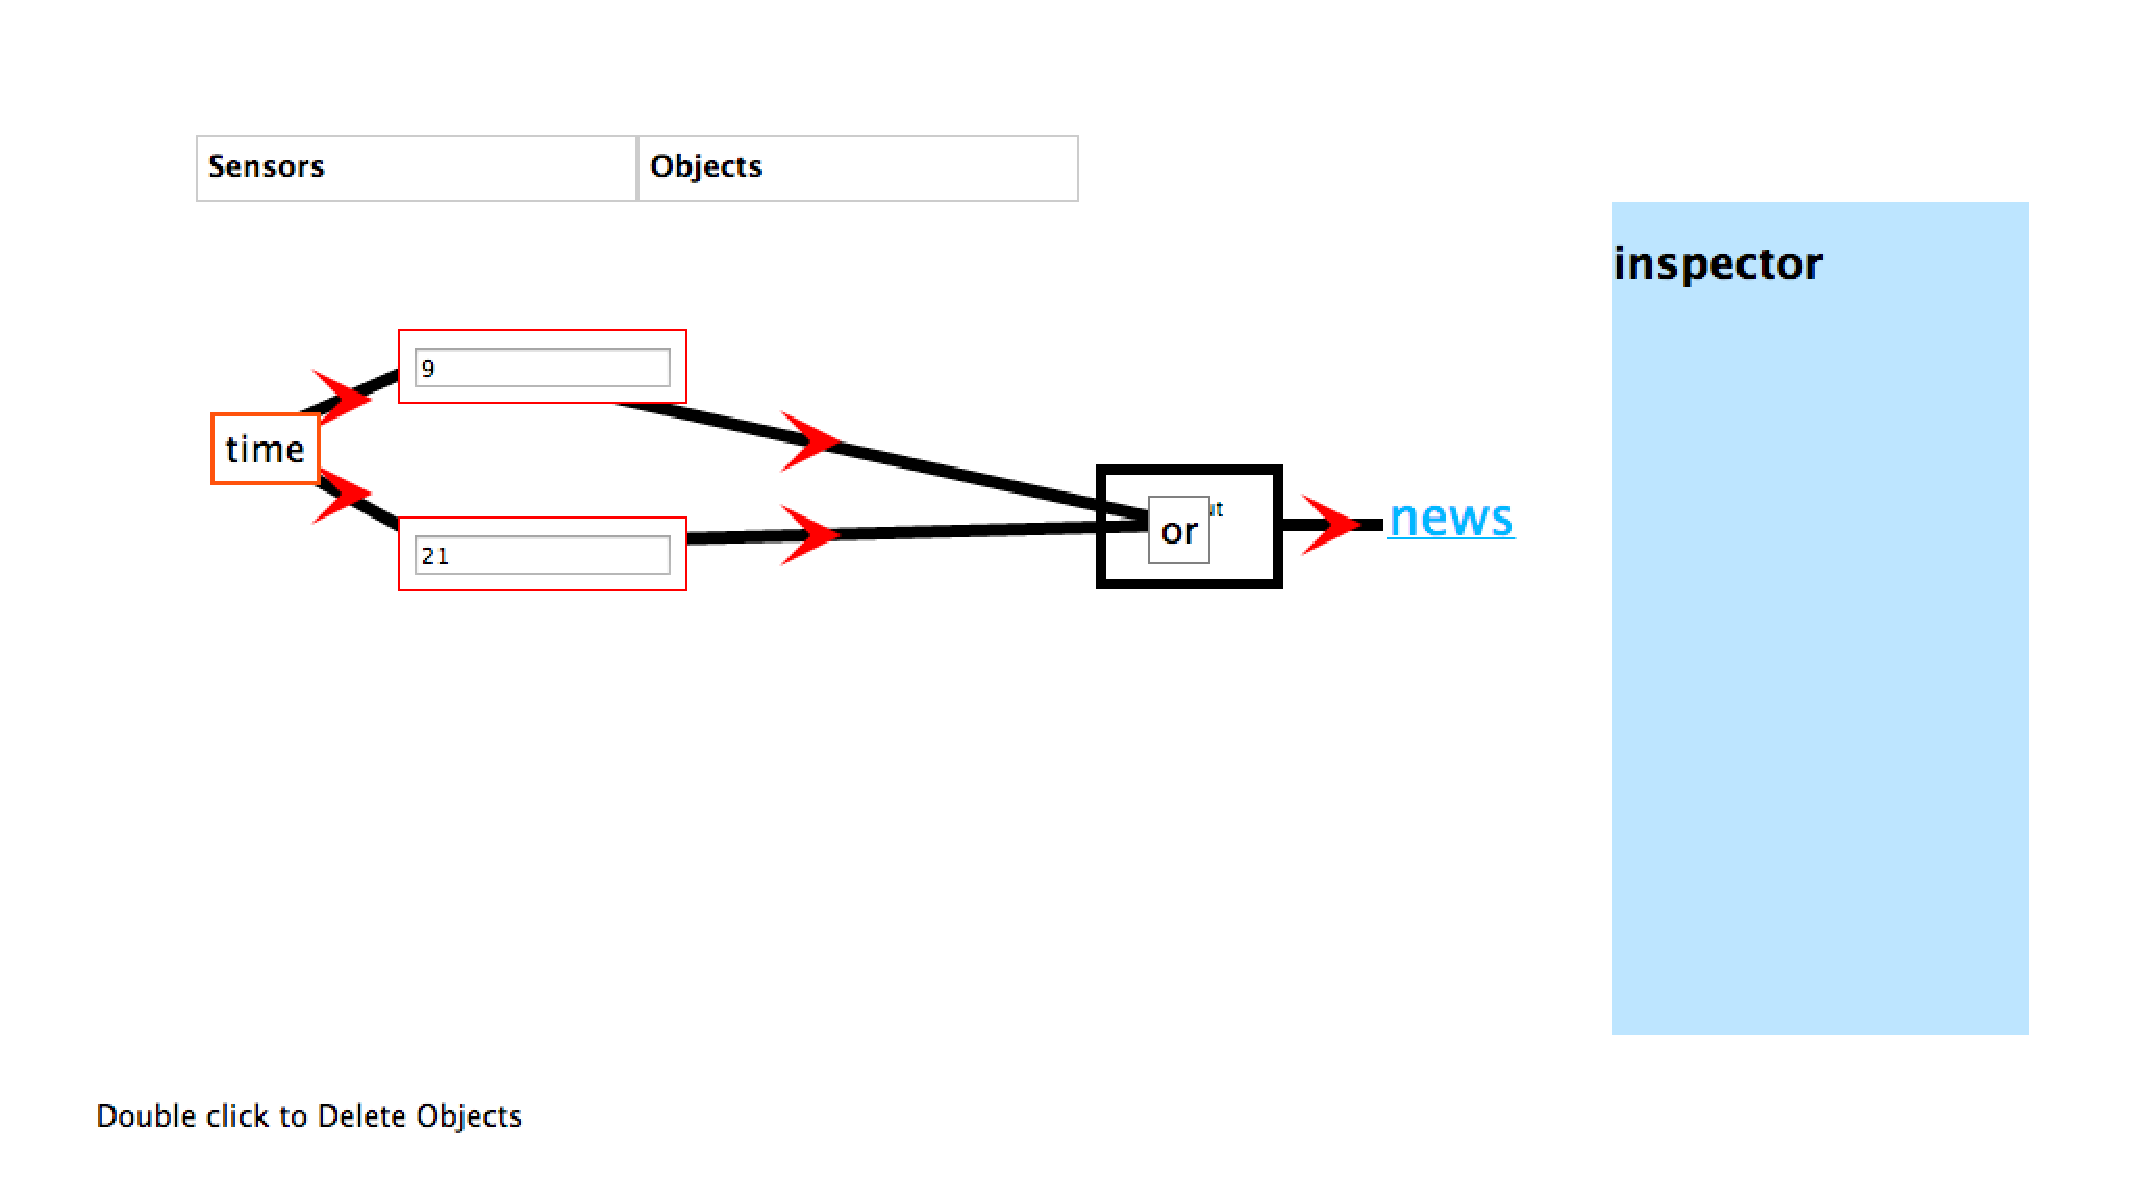
\includegraphics[width=150mm]{image/image10.eps}}
  \end{center}
  \caption{ニュースの購読をビジュアルプログラミング}
  \label{fig:image10}
\end{figure}

\section{超自動ドア}
携帯の位置情報とエレベーターで人があがってきたことをセンシングする。エレベーターがあがってきたという条件と携帯の位置が付近に来たことが送られてくると自動でドアが開く。(図\ref{fig:image14})のようにPOSTリクエストでドアをあける機構を作っておくことで実装可能だ。
(図\ref{fig:image11})はCellPhone\_lonというオブジェクトとCellPhone\_latというオブジェクトがそれぞれ緯度と経度を取得してきている。これをelevatorのデータとマージし、マッチした時にdoorにアクセスしている。
\begin{figure}[htbp]
  \begin{center}
    \fbox{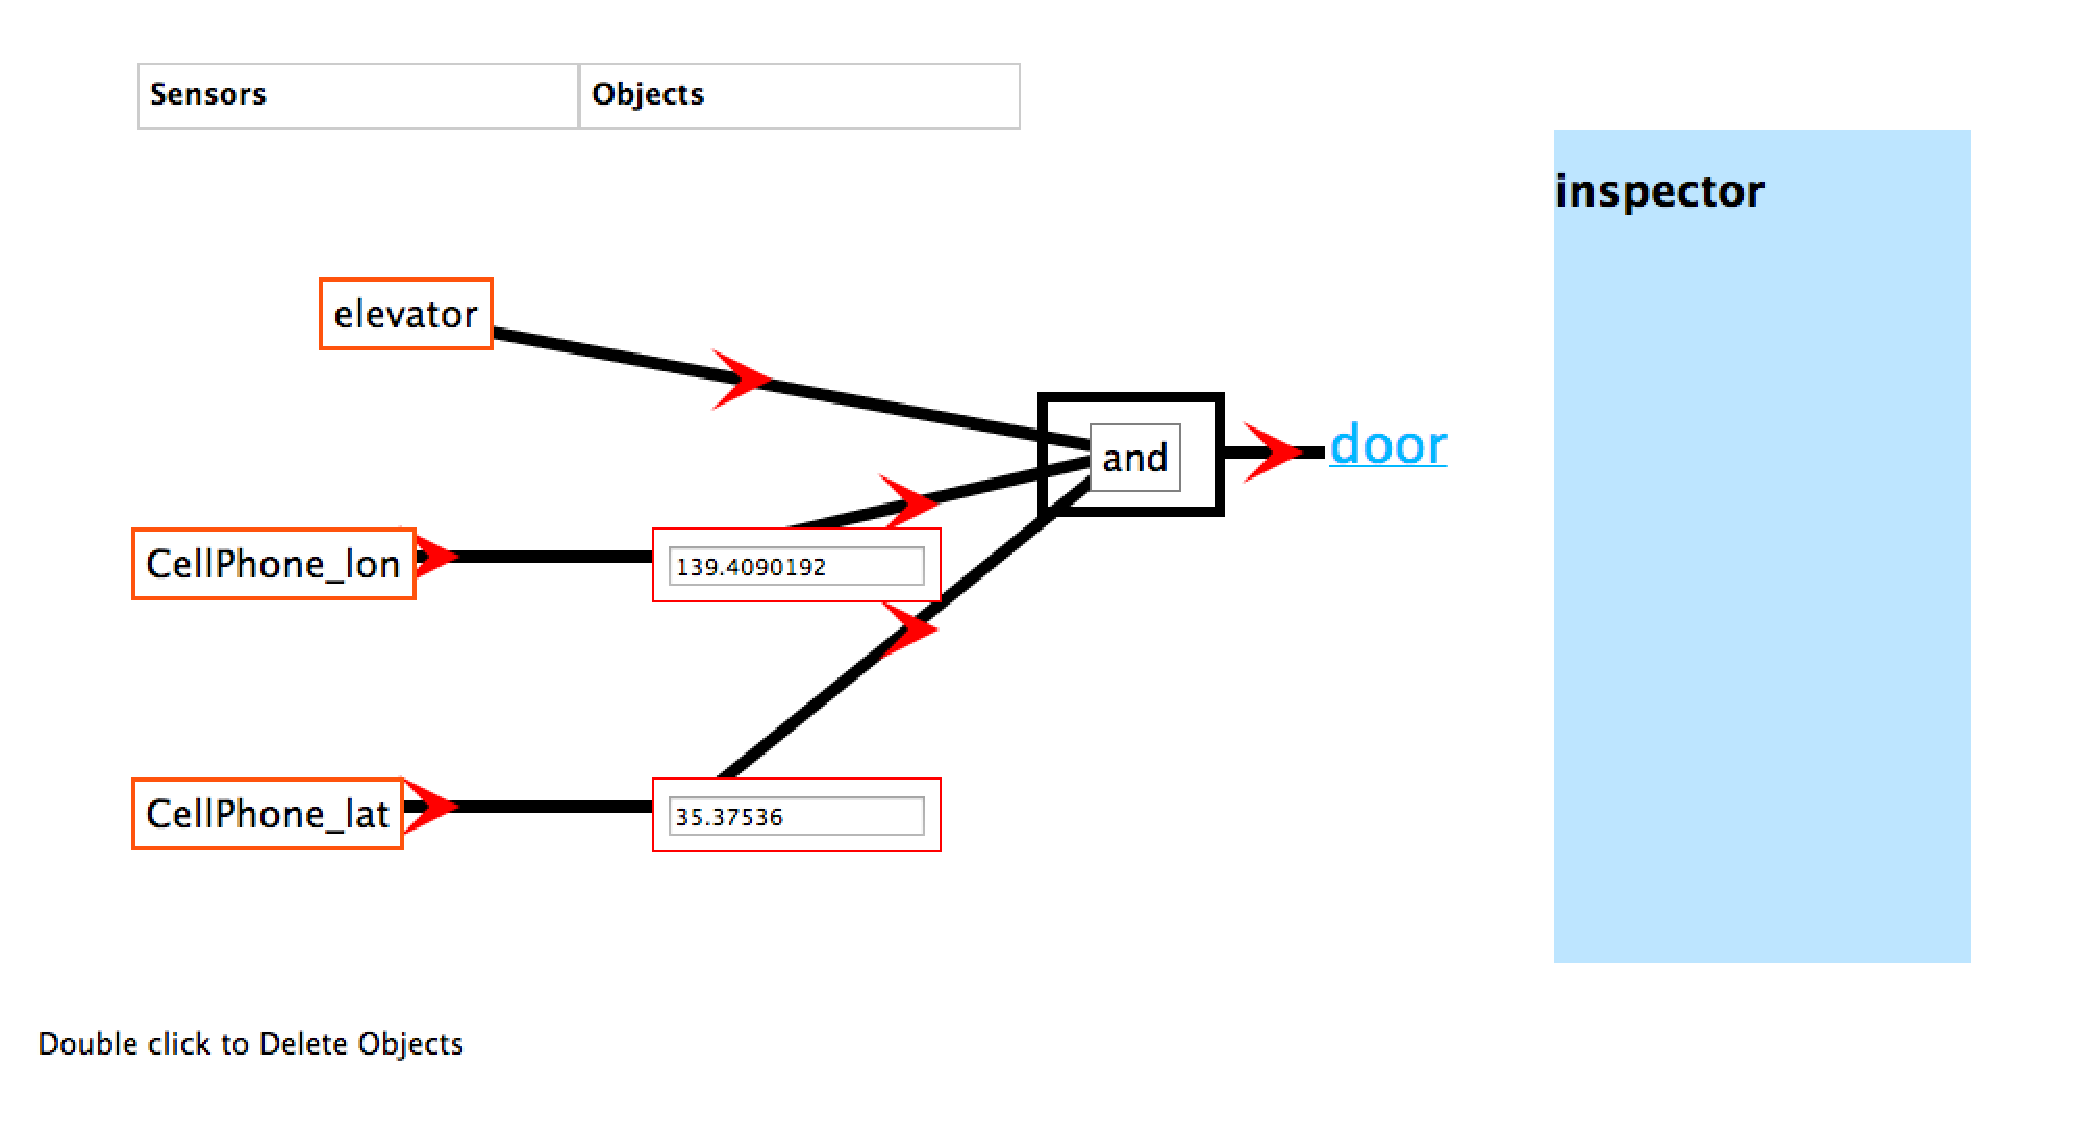
\includegraphics[width=150mm]{image/image11.eps}}
  \end{center}
  \caption{超自動ドアをビジュアルプログラミング}
  \label{fig:image11}
\end{figure}

\begin{figure}[htbp]
  \begin{center}
    \fbox{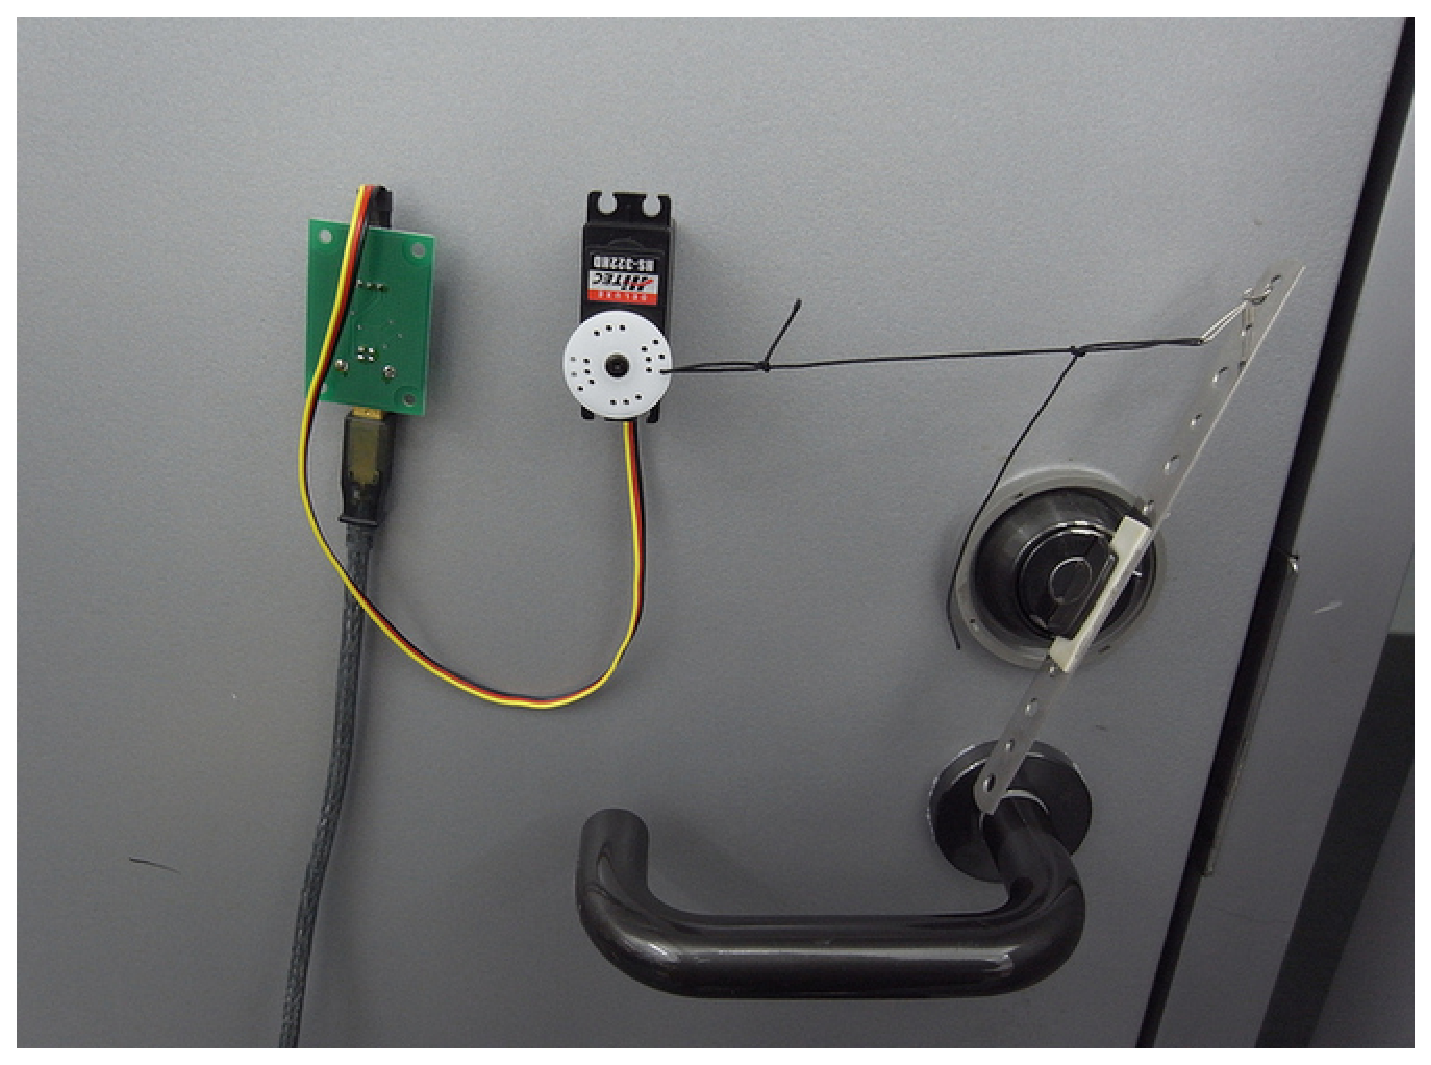
\includegraphics[width=80mm]{image/image14.eps}}
  \end{center}
  \caption{自動解錠するための機構}
  \label{fig:image14}
\end{figure}

\section{忘れ物を通知}
ドアが開いたかどうか、と鞄の中に特定の物があるかというセンシングデータを組み合わせる。ドアが開いた時に鞄の中に物がなかった場合のみ通知をくるように設定し、忘れ物を防止することができる。
(図\ref{fig:image12})のInBagオブジェクトはRFIDタグ\footnote{固有のID情報を埋め込めるタグ}を鞄に設置し、登録した物の有無を検出する。一定時間でtrue/falseを判定し、trueの時だけイベントを発火する。そしてドアが開いた時に鞄の中の財布の有無を確認し、通知することができる。
\begin{figure}[htbp]
  \begin{center}
    \fbox{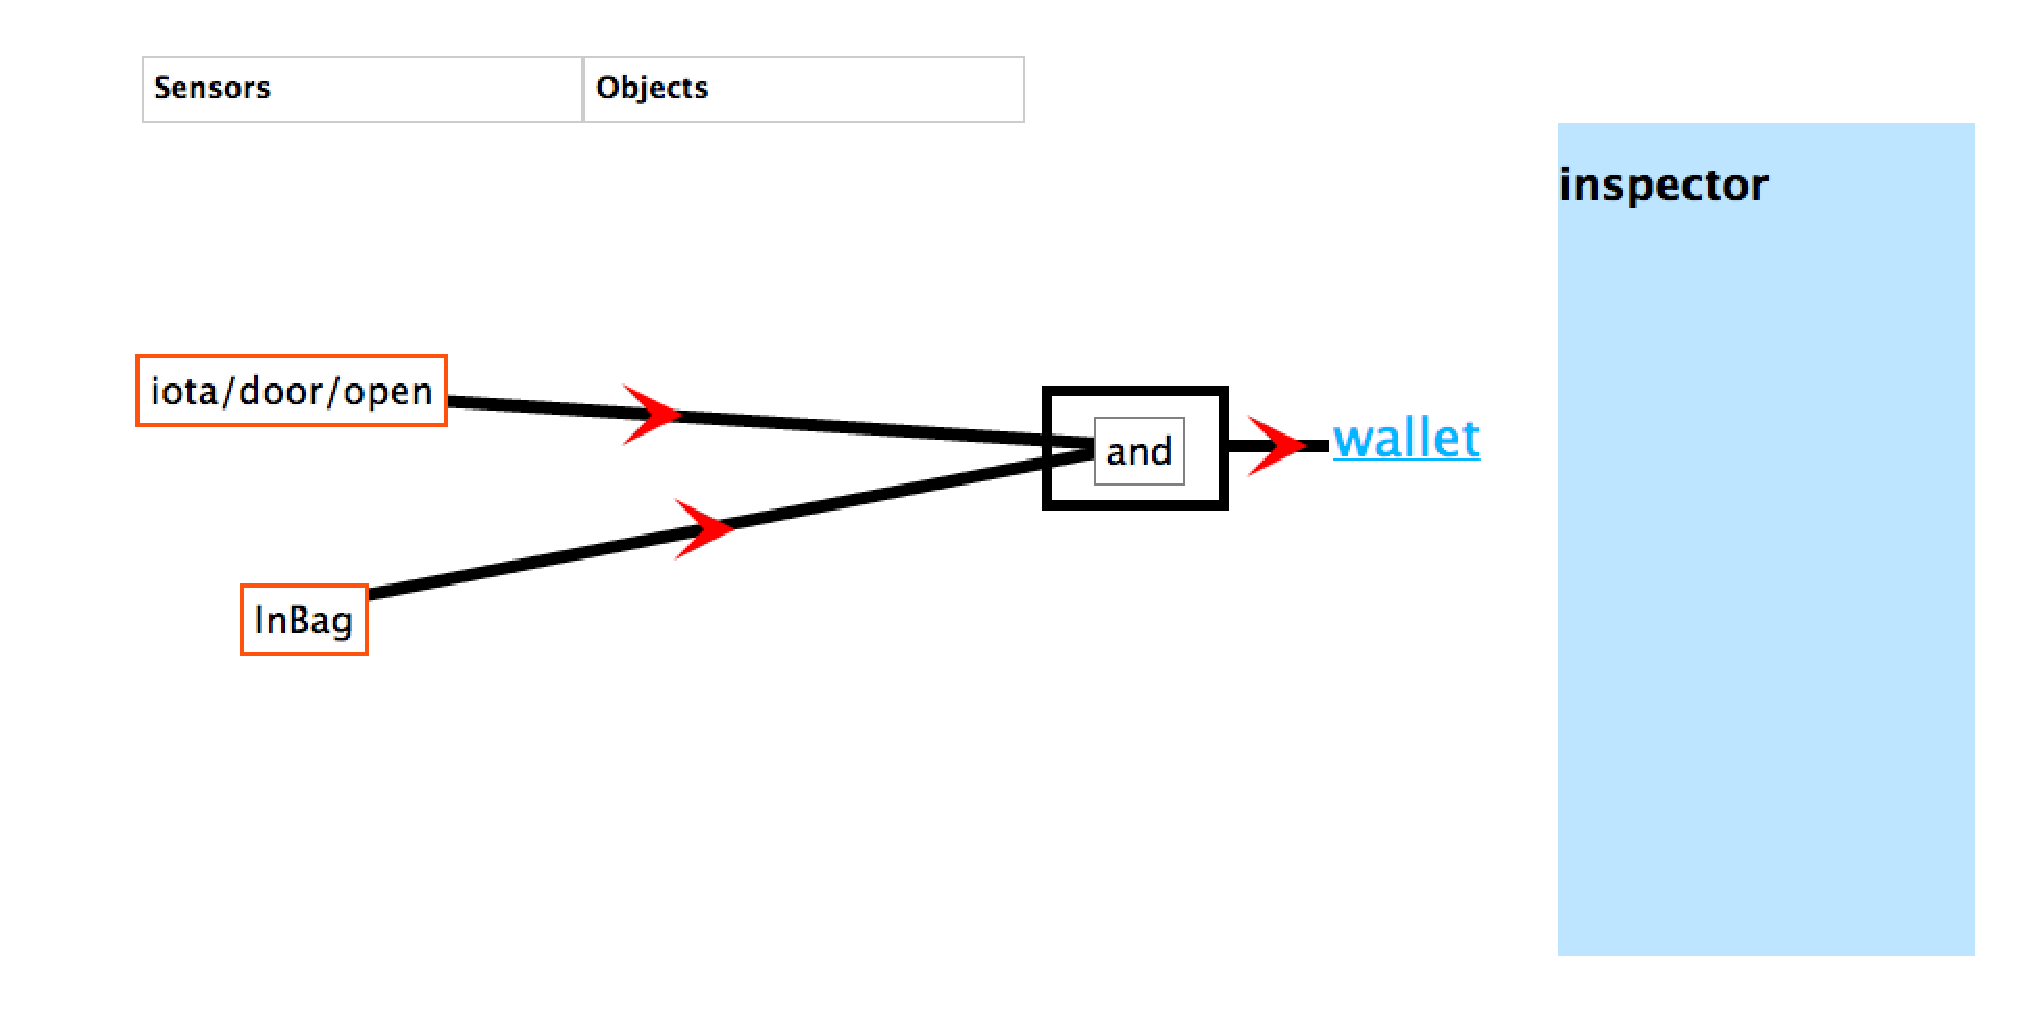
\includegraphics[width=150mm]{image/image12.eps}}
  \end{center}
  \caption{忘れ物検知をビジュアルプログラミング}
  \label{fig:image12}
\end{figure}

\section{カビを通知}
風呂場などに設置するといいだろう。その場所の温度と湿度をセンシングし、カビの発生条件に近いデータにマッチしたらイベントを発火する。また、壁を一定時間ごとに撮影し色の変化を観察することで精度をあげることが出来る。
(図\ref{fig:image13})では温度、湿度、壁の色という3つの要素でカビが発生しそうかどうか判定している。上から、温度20℃から30℃にマッチしたtrue、湿度が80%以上だったらtrue、壁の写真の色平均をとり、RGBの合計が100以下になったら黒ずんできたと判断しtrueとしている。
写真はRaspberry Pi\footnote{http://www.raspberrypi.org/}にWebカメラをつけ、定期的に色平均を計算させている。(図\ref{fig:image15})
\begin{figure}[htbp]
  \begin{center}
    \fbox{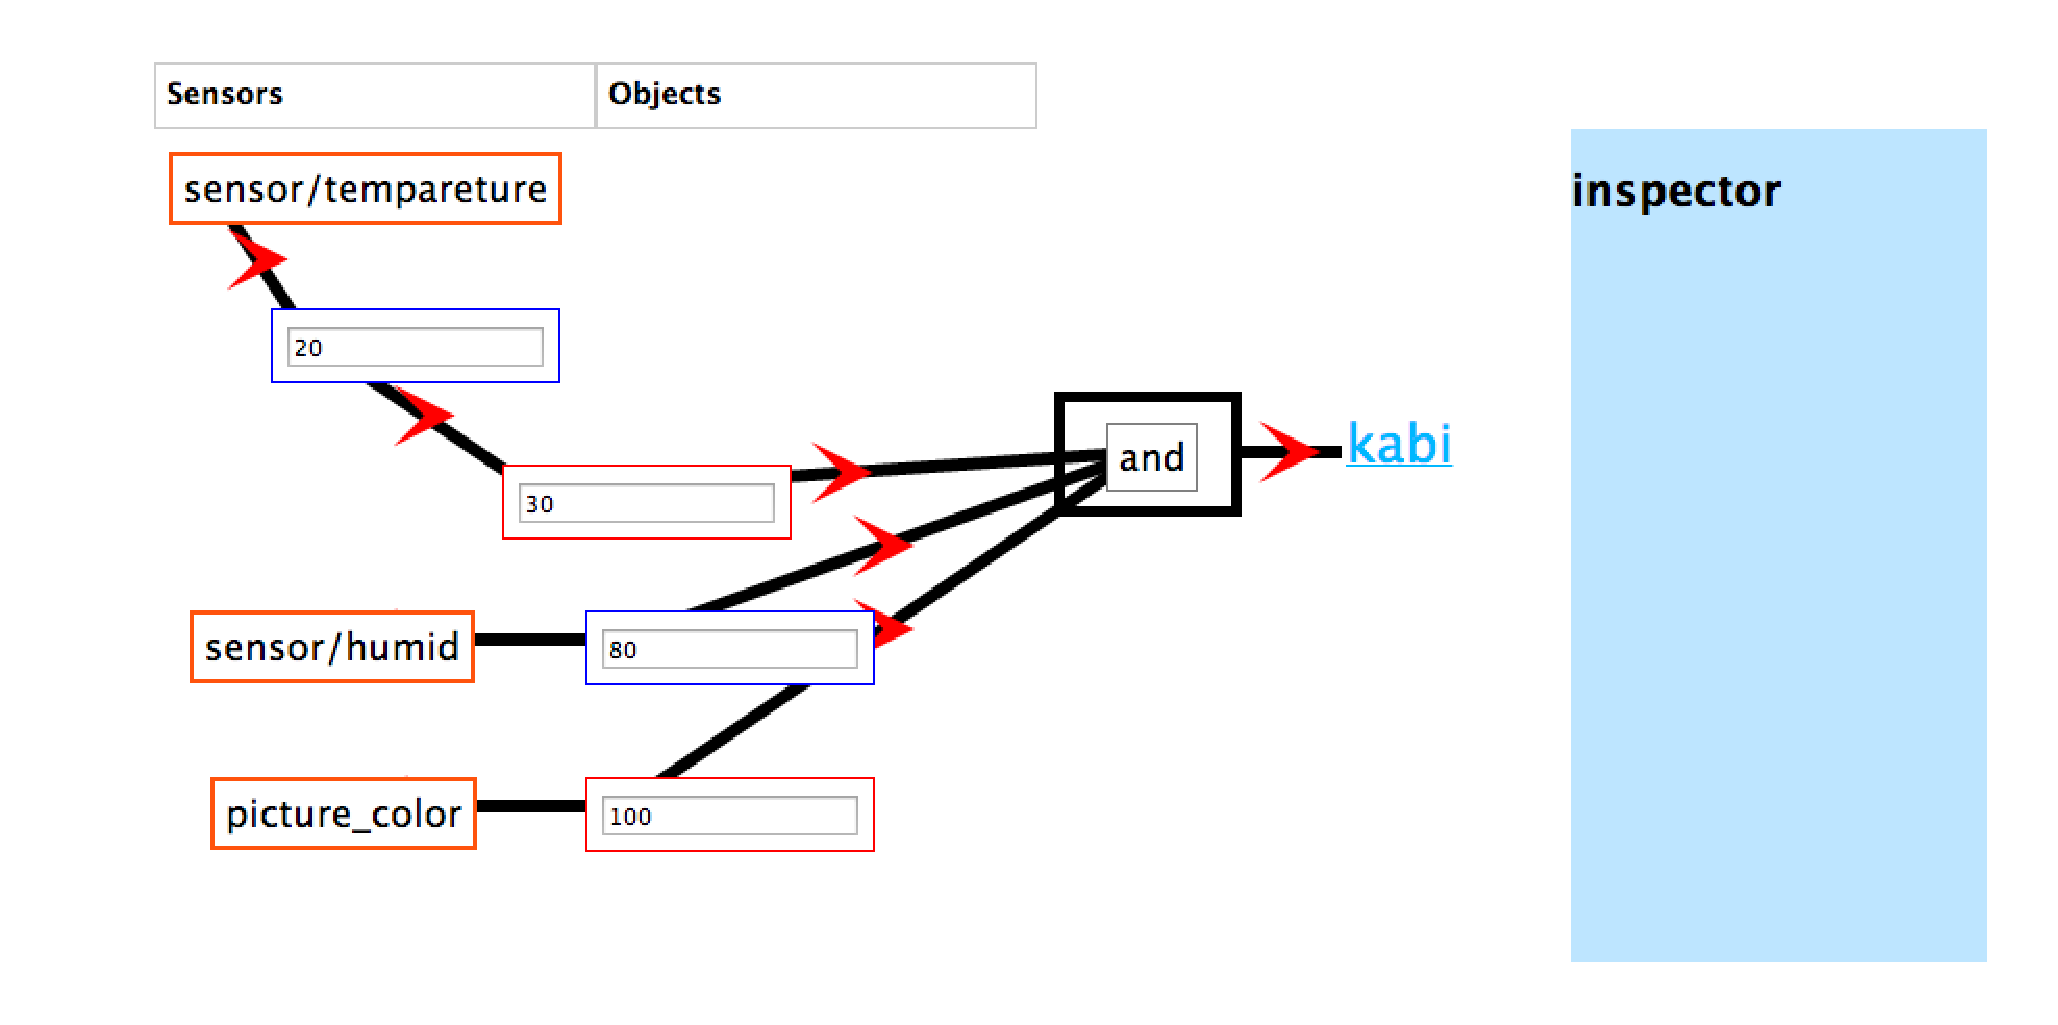
\includegraphics[width=150mm]{image/image13.eps}}
  \end{center}
  \caption{カビの通知をビジュアルプログラミング}
  \label{fig:image13}
\end{figure}

\begin{figure}[htbp]
  \begin{center}
    \fbox{\includegraphics[width=80mm]{image/image15.eps}}
  \end{center}
  \caption{壁の写真をとるための機構}
  \label{fig:image15}
\end{figure}

\section{朝食自動調理}
様々な条件に従って自動で料理を作ってくれるということも簡単にできるだろう。そもそも現状、炊飯器などにタイマーがついていて家電は色々な形で条件指定することができる。Web上で家電を管理することができれば人数や気温、季節、時間など複数の条件分岐を作成すれば複雑な条件で処理させることが可能だろう。
	% 本文4
\end{verbatim}
\end{itembox}

目次に続いて、論文のメイン、本文を記述する。アブストラクトと同様で、{\tt main.tex}に直接書くか、\verb|\include| コマンドを利用して別に用意したファイルを{\tt include}する。

本文の書き方は、第\ref{chap:latex}章で詳しく説明する。


\subsection{謝辞の出力}

\begin{itembox}[l]{{\tt main.tex}}
\begin{verbatim}
\begin{acknowledgment}
本研究を進めるにあたり、ご指導くださった増井俊之先生に深く感謝いたします。
アイデアの出し方、研究の進め方、実装方法など多くのことを学ばせていただきました。

橋本翔氏にはプログラミングの方法など、多くのことを学ばせて頂きました。ありがとうございました。

また、研究を進めるにあたり、増井研究室の皆様に多くのアドバイスを頂きました。心より感謝しております。\\\\
最後に学生生活を支えてくださった家族に感謝いたします。

\begin{flushright}
永倉 啓太
\end{flushright}

\end{acknowledgment}
	% 謝辞。要独自コマンド、include先参照のこと
\end{verbatim}
\end{itembox}

本文のあとには、謝辞を出力する。\verb|begin{acknowledgment}| から \verb|end{acknowledgment}| の間に書いた文章が、謝辞として独立したページに出力される。アブストラクトや本文と同じで、{\tt main.tex}に直接書いてもよいし、\verb|\include| コマンドを利用して{\tt include}してもよい。


\subsection{参考文献の出力}

\begin{itembox}[l]{{\tt main.tex}}
\begin{verbatim}
\include{91_bibliography}	% 参考文献。要独自コマンド、include先参照のこと
\end{verbatim}
\end{itembox}

謝辞に続いて、参考文献を出力する。

参考文献リストは、\verb|\begin{bib}| から \verb|\end{bib}| の間に、\verb|\bibitem| コマンドを使って書く。

BibTeXを使う場合は、以下のようにする。

\begin{itembox}[l]{{\tt 91\_bibliography.tex}}
\begin{verbatim}
\begin{bib}[100]
\bibliography{main}
\end{bib}
\end{verbatim}
\end{itembox}

こうすると、\verb|main.bib|から使用した参考文献のみを抽出して出力してくれる。\verb|main.bib|の中身は以下のようになっていて、気の利いた論文検索サイトであればBibTeXをコピペできるようになっているので簡単に作れるはず。


\begin{itembox}[l]{{\tt 91\_bibliography.tex}}
\begin{verbatim}
@article{hoge09,
    author  = "ほげ山太郎 and ほげ山次郎",
    yomi    = "ほげやまたろう",
    title   = "ほげほげ理論のHCI分野への応用",
    journal = "ほげほげ学会論文誌",
    volume  = "31",
    number  = "3",
    pages   = "194-201",
    year    = "2009",
}
@inproceedings{hoge08,
    author     = "Taro Hogeyama and Jiro Hogeyama",
    title      = "The Theory of Hoge",
    booktitle  = "The Proceedings of The Hoge Society",
    year       = "2008"
}
\end{verbatim}
\end{itembox}


以下は、BibTeXを使わないで手で書く例。

\begin{itembox}[l]{{\tt 91\_bibliography.tex}}
\begin{verbatim}
@article{hoge09,
    author  = "ほげ山太郎 and ほげ山次郎",
    yomi    = "ほげやまたろう",
    title   = "ほげほげ理論のHCI分野への応用",
    journal = "ほげほげ学会論文誌",
    volume  = "31",
    number  = "3",
    pages   = "194-201",
    year    = "2009",
}
@inproceedings{hoge08,
    author     = "Taro Hogeyama and Jiro Hogeyama",
    title      = "The Theory of Hoge",
    booktitle  = "The Proceedings of The Hoge Society",
    year       = "2008"
}
\end{verbatim}
\end{itembox}


英語の文献の場合、慣例的に書誌名をイタリック体にすることが多いらしい。

\begin{itembox}[l]{{\tt 91\_bibliography.tex}}
\begin{verbatim}
\begin{bib}[100]
\begin{thebibliography}{#1}
% \bibitem{参照用名称}
%   著者名:
%   \newblock 文献名,
%   \newblock 書誌情報,出版年.

\bibitem{hoge09}
  ほげ山太郎,ほげ山次郎:
  \newblock ほげほげ理論のHCI分野への応用,
  \newblock ほげほげ学会論文誌,Vol.31,No.3,pp.194-201,2009.

\bibitem{hoge08}
  Taro Hogeyama, Jiro Hogeyama:
  \newblock The Theory of Hoge,
  \newblock {\it The Proceedings of The Hoge Society}, 2008.
\end{thebibliography}
\end{bib}
\end{verbatim}
\end{itembox}

\verb|\bibitem| コマンド中、参照用名称は、本文から参考文献を参照するときに使うので、忘れずに書いておく。参照文献を本文中に参照するときには、\verb|\cite{参照用名称}| のように書けばよい。例えば、この文の末尾には \verb|\cite{hoge09}| と書いてあるので、自動で対応する番号が振られる\cite{hoge09}\cite{hoge08}。

参考文献リストの番号付けと、本文で参照したときの番号の挿入は、全部が自動で行われる。ただしこれも、第\ref{sec:toc}節で説明した目次の出力と同じで、一時ファイルを生成してからの挿入なので、正しく出力するには最低でも二回のコンパイルが必要。BibTeXを使用する場合は、\verb|platex|コマンドのあと\verb|pbibtex|コマンドを実行し、さらに2回\verb|platex|コマンドを実行するといいらしい。



\subsection{付録の出力}

\begin{itembox}[l]{{\tt main.tex}}
\begin{verbatim}
\appendix
\include{92_appendix}		% 付録
\end{verbatim}
\end{itembox}

必要であれば、論文の最後には付録を出力する。

\verb|\appendix| コマンド以降に書いたものは、すべて付録として扱われる。付録部分の書き方は通常の本文とまったく同じで、\verb|\appendix| コマンド以降に書くだけで勝手に付録用の体裁で出力される。
	% 本文2
\chapter{プロトタイプの実装}
\label{chap:prototype}

この章では本研究でのプロトタイプを実装し、その流れを解説する。

\section{実装概要}
大量のデータをやりとりすることを想定してnode.js\footnote{http://www.nodejs.org/}で実装した。またデータベースはmongoDB\footnote{http://www.mongodb.org/}を採用し、軽量フレームワークを実現した。元になっているセンサーデータはLindaを利用し、データを取得、書き込みしている。

クライアントサイドではJQuery UI\footnote{http://jqueryui.com/}とSVG\footnote{http://www.w3.org/Graphics/SVG/}を使い、ドラッグ&ドロップと線の描画を実現している。

\section{ページ遷移}
パスによってページを管理している。基本的にはパスの名前が最終的に結びつけるオブジェクトの名前になっている。パスにアクセスした際、オブジェクトが作成されていなかった場合には新しいオブジェクトの作成が促され、データベースに記録される。ユーザーはそのオブジェクトに対してアクションとその条件を指定することでプログラムしていく。/keyというページに最初にアクセスした際にはkeyオブジェクトを作成する。最終的なアクションは/key/outputでPOST送信先を設定する。例えば部屋の明るさをセンシングし、部屋が暗くなったらという条件をkeyオブジェクトに紐付け、携帯に通知を送るというアクションを実行することなどができる。その他にも鍵の開け閉めをWebで管理している場合にはそのURLにリクエストを送ることもできる。

/controlのパスはデータベースの管理ができるようになっており、センサーやオブジェクトに追加が出来るようになっている。


\section{サーバーサイド}
言語はJavascriptを使い、node.jsのsocket.io\footnote{http://socket.io/}で実装した。センサーオブジェクトに対して常にコネクションを貼り、データをemitしている。mongoDBではセンサーデータ、オブジェクトデータ、コネクションデータ、クライアントデータを保存している。

\section{クライアントサイド}
クライアントサイドもサーバーサイドと同様にJavascriptを選択した。ページ内でオブジェクトの作成、移動、コネクションの作成などのアクションが行われた際に常にサーバー側に情報を送り保存している。イベントの制御にはEvent Emitter\footnote{http://nodejs.org/api/events.html}を用いた。Event Emitterを使えばオブジェクト自体にイベントを持たせることができる。それぞれのオブジェクトが送られてきたデータを監視し、自分の持っている条件にマッチしたら自らが送信側になるという実装をしている。下の図ではdelta/sensor/lightというセンサーを親データとして、orというオブジェクトが監視して条件に照らし合わせマッチしたら発信するオブジェクトになっている。(図\ref{fig:image09})

\begin{figure}[htbp]
  \begin{center}
    \fbox{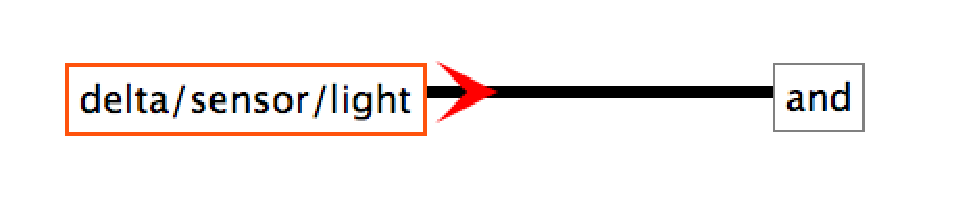
\includegraphics[width=100mm]{image/image09.eps}}
  \end{center}
  \caption{センサーデータの親子関係}
  \label{fig:image09}
\end{figure}

	% 本文3
\chapter{利用法}
\label{chap:usage}
この章ではセンシングデータの利用法を具体的に提案する。\\
センシングデータといってもWeb上で取得できる物は全てデータとして扱うことが出来る。
例えば藤沢の気温データをWeb上から更新される度に取得することで気温のセンシングデータを作成できる。また、現在時刻やPCのファイル情報などユーザーのコンテキストも取得してデータにすることが出来る。
これらのデータを使えば条件指定の幅が広がり複雑なプログラムを簡単に書くことが出来る。

\section{ニュース購読}
現在時刻を取得することで簡単にアラーム機能を実装できる。指定の時間をすぎるとニュースを取得し、PCに喋らせているのが以下の例だ。Macのsayコマンドを使って特定のPCから音声を発信している。
(図\ref{fig:image10})では時間を取得するtimeオブジェクトが9時と21時にマッチした時にnewsにアクセスしている。
\begin{figure}[htbp]
  \begin{center}
    \fbox{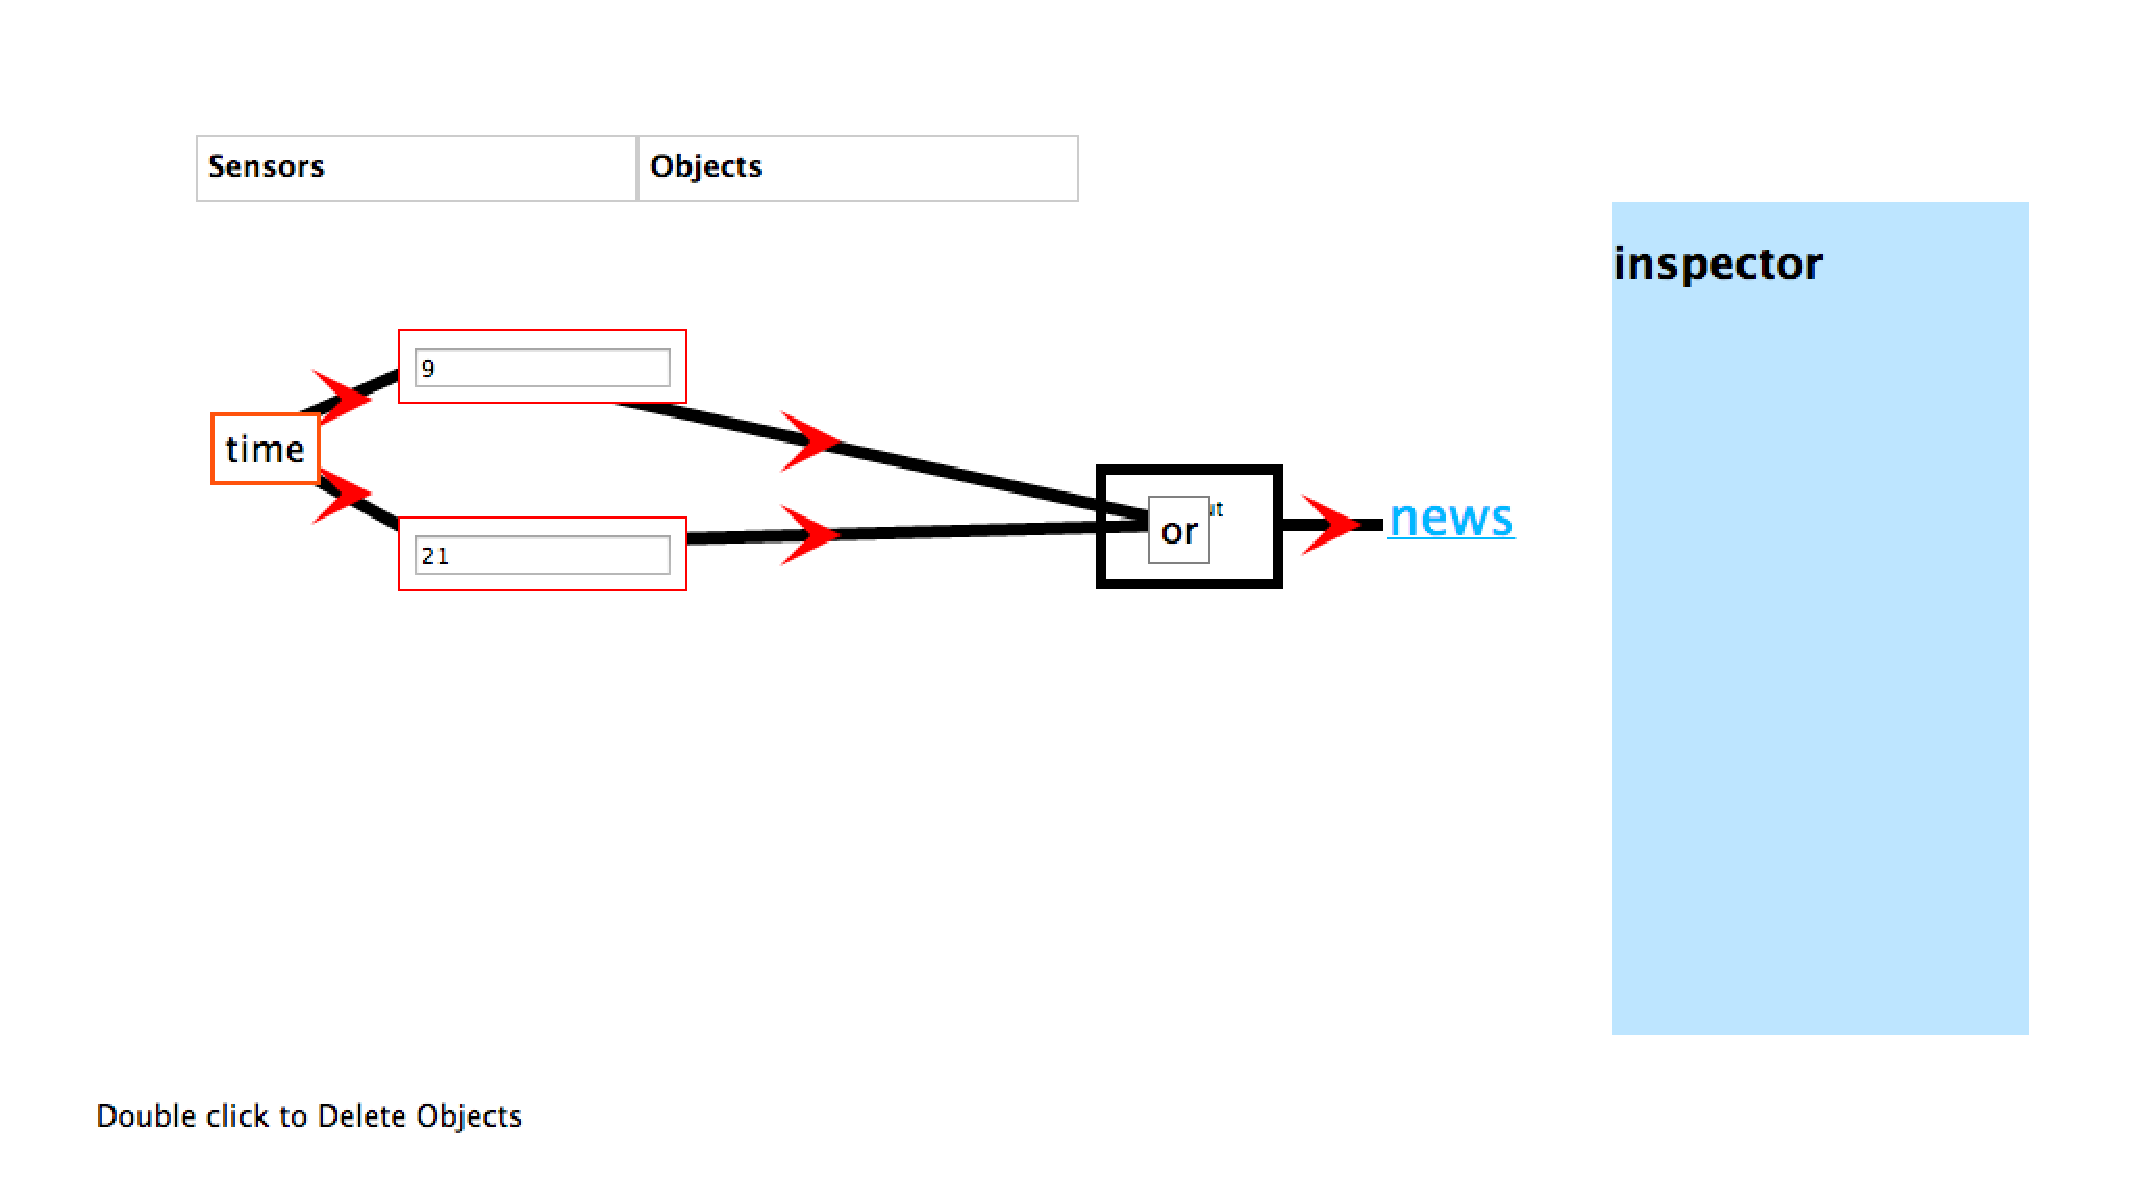
\includegraphics[width=150mm]{image/image10.eps}}
  \end{center}
  \caption{ニュースの購読をビジュアルプログラミング}
  \label{fig:image10}
\end{figure}

\section{超自動ドア}
携帯の位置情報とエレベーターで人があがってきたことをセンシングする。エレベーターがあがってきたという条件と携帯の位置が付近に来たことが送られてくると自動でドアが開く。(図\ref{fig:image14})のようにPOSTリクエストでドアをあける機構を作っておくことで実装可能だ。
(図\ref{fig:image11})はCellPhone\_lonというオブジェクトとCellPhone\_latというオブジェクトがそれぞれ緯度と経度を取得してきている。これをelevatorのデータとマージし、マッチした時にdoorにアクセスしている。
\begin{figure}[htbp]
  \begin{center}
    \fbox{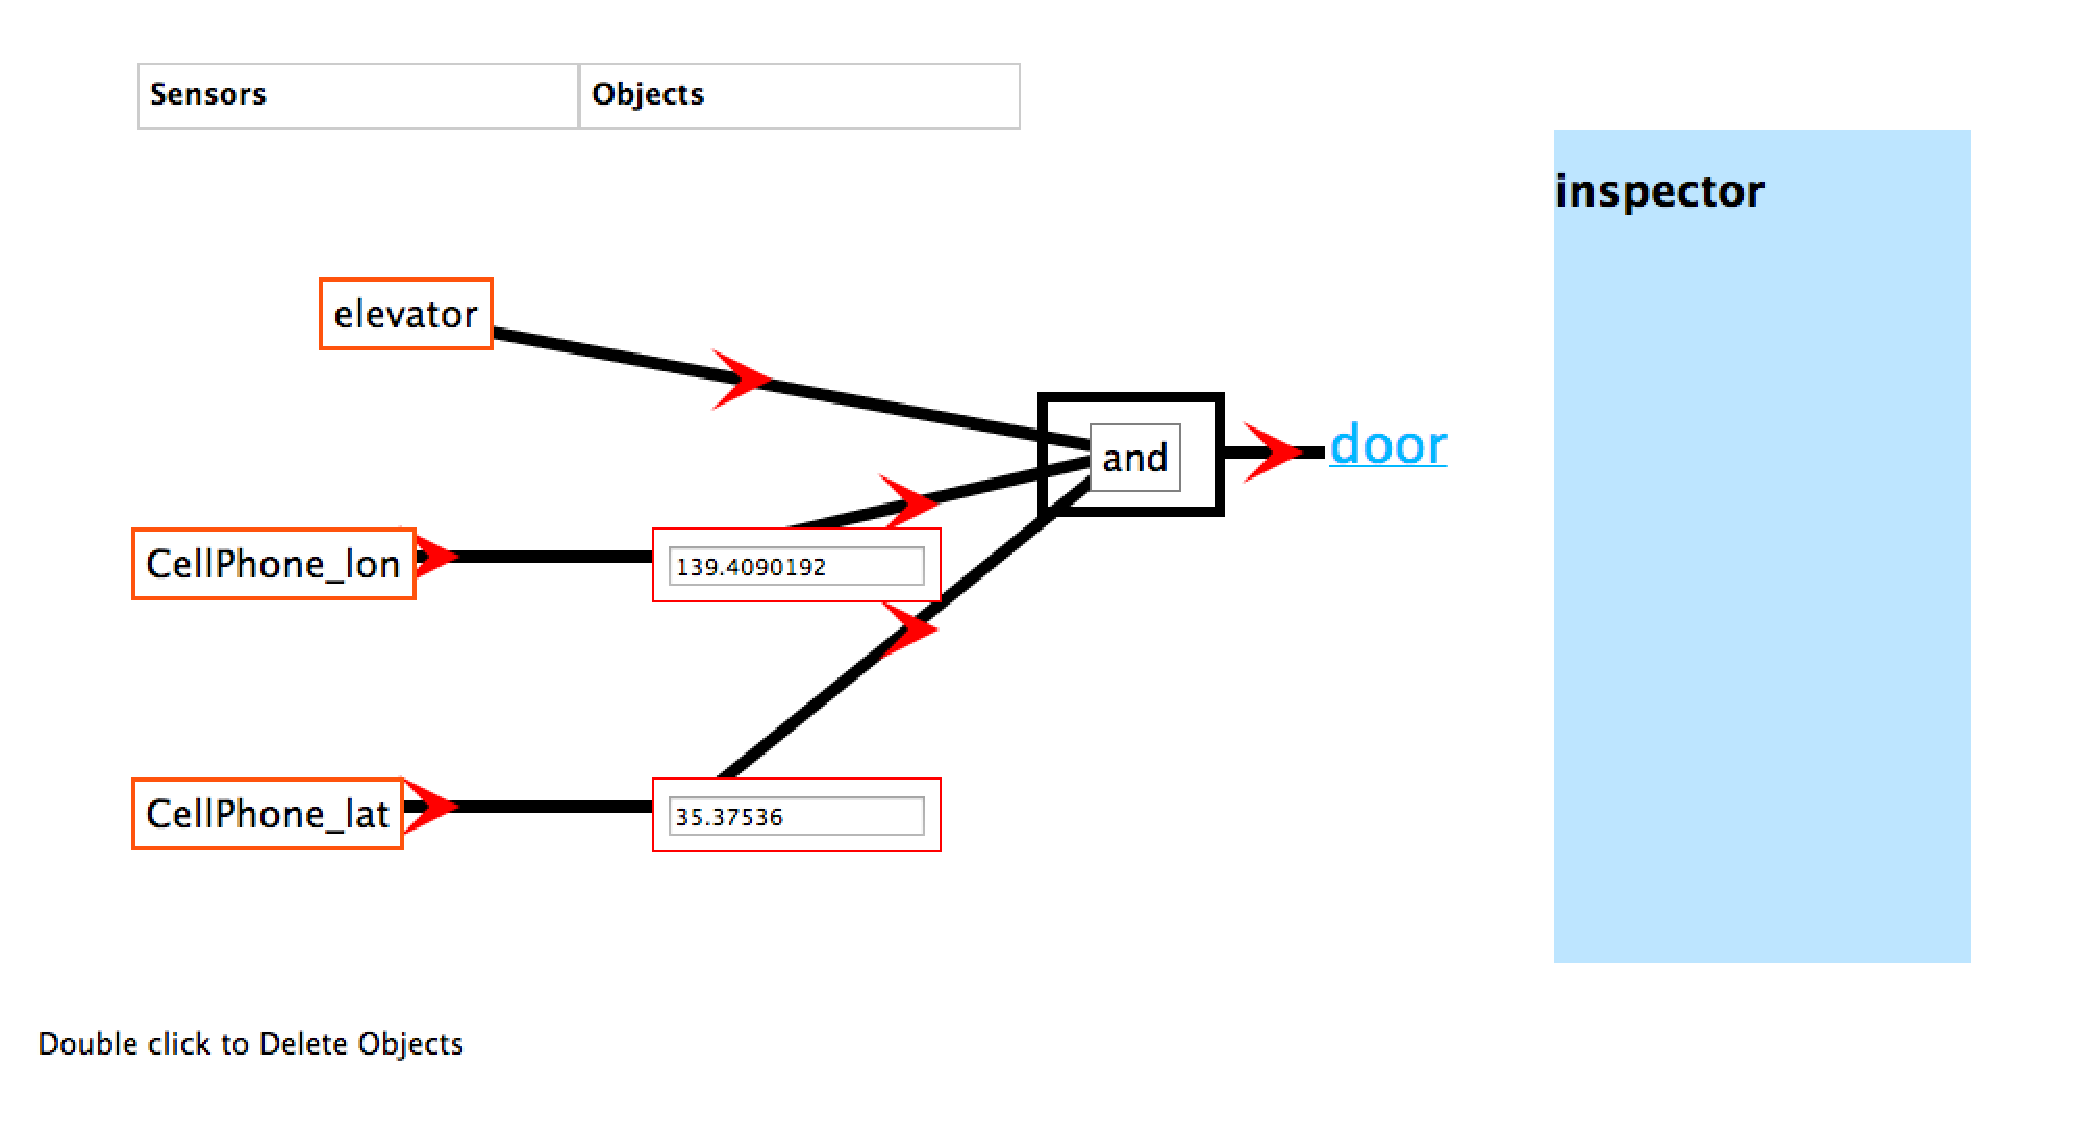
\includegraphics[width=150mm]{image/image11.eps}}
  \end{center}
  \caption{超自動ドアをビジュアルプログラミング}
  \label{fig:image11}
\end{figure}

\begin{figure}[htbp]
  \begin{center}
    \fbox{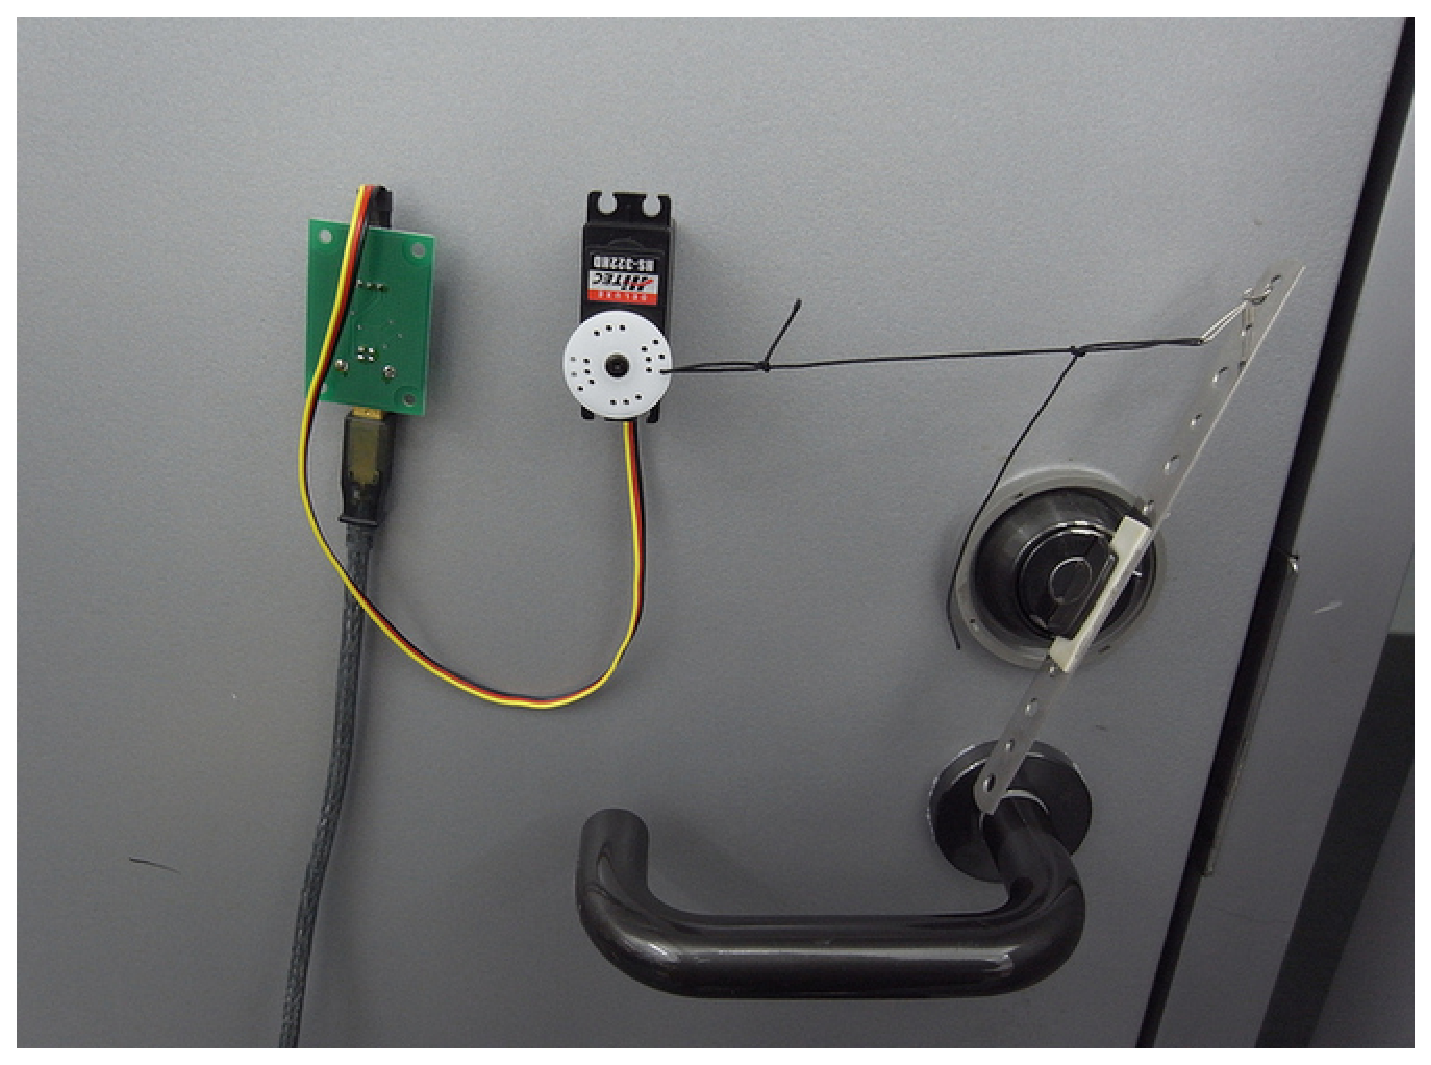
\includegraphics[width=80mm]{image/image14.eps}}
  \end{center}
  \caption{自動解錠するための機構}
  \label{fig:image14}
\end{figure}

\section{忘れ物を通知}
ドアが開いたかどうか、と鞄の中に特定の物があるかというセンシングデータを組み合わせる。ドアが開いた時に鞄の中に物がなかった場合のみ通知をくるように設定し、忘れ物を防止することができる。
(図\ref{fig:image12})のInBagオブジェクトはRFIDタグ\footnote{固有のID情報を埋め込めるタグ}を鞄に設置し、登録した物の有無を検出する。一定時間でtrue/falseを判定し、trueの時だけイベントを発火する。そしてドアが開いた時に鞄の中の財布の有無を確認し、通知することができる。
\begin{figure}[htbp]
  \begin{center}
    \fbox{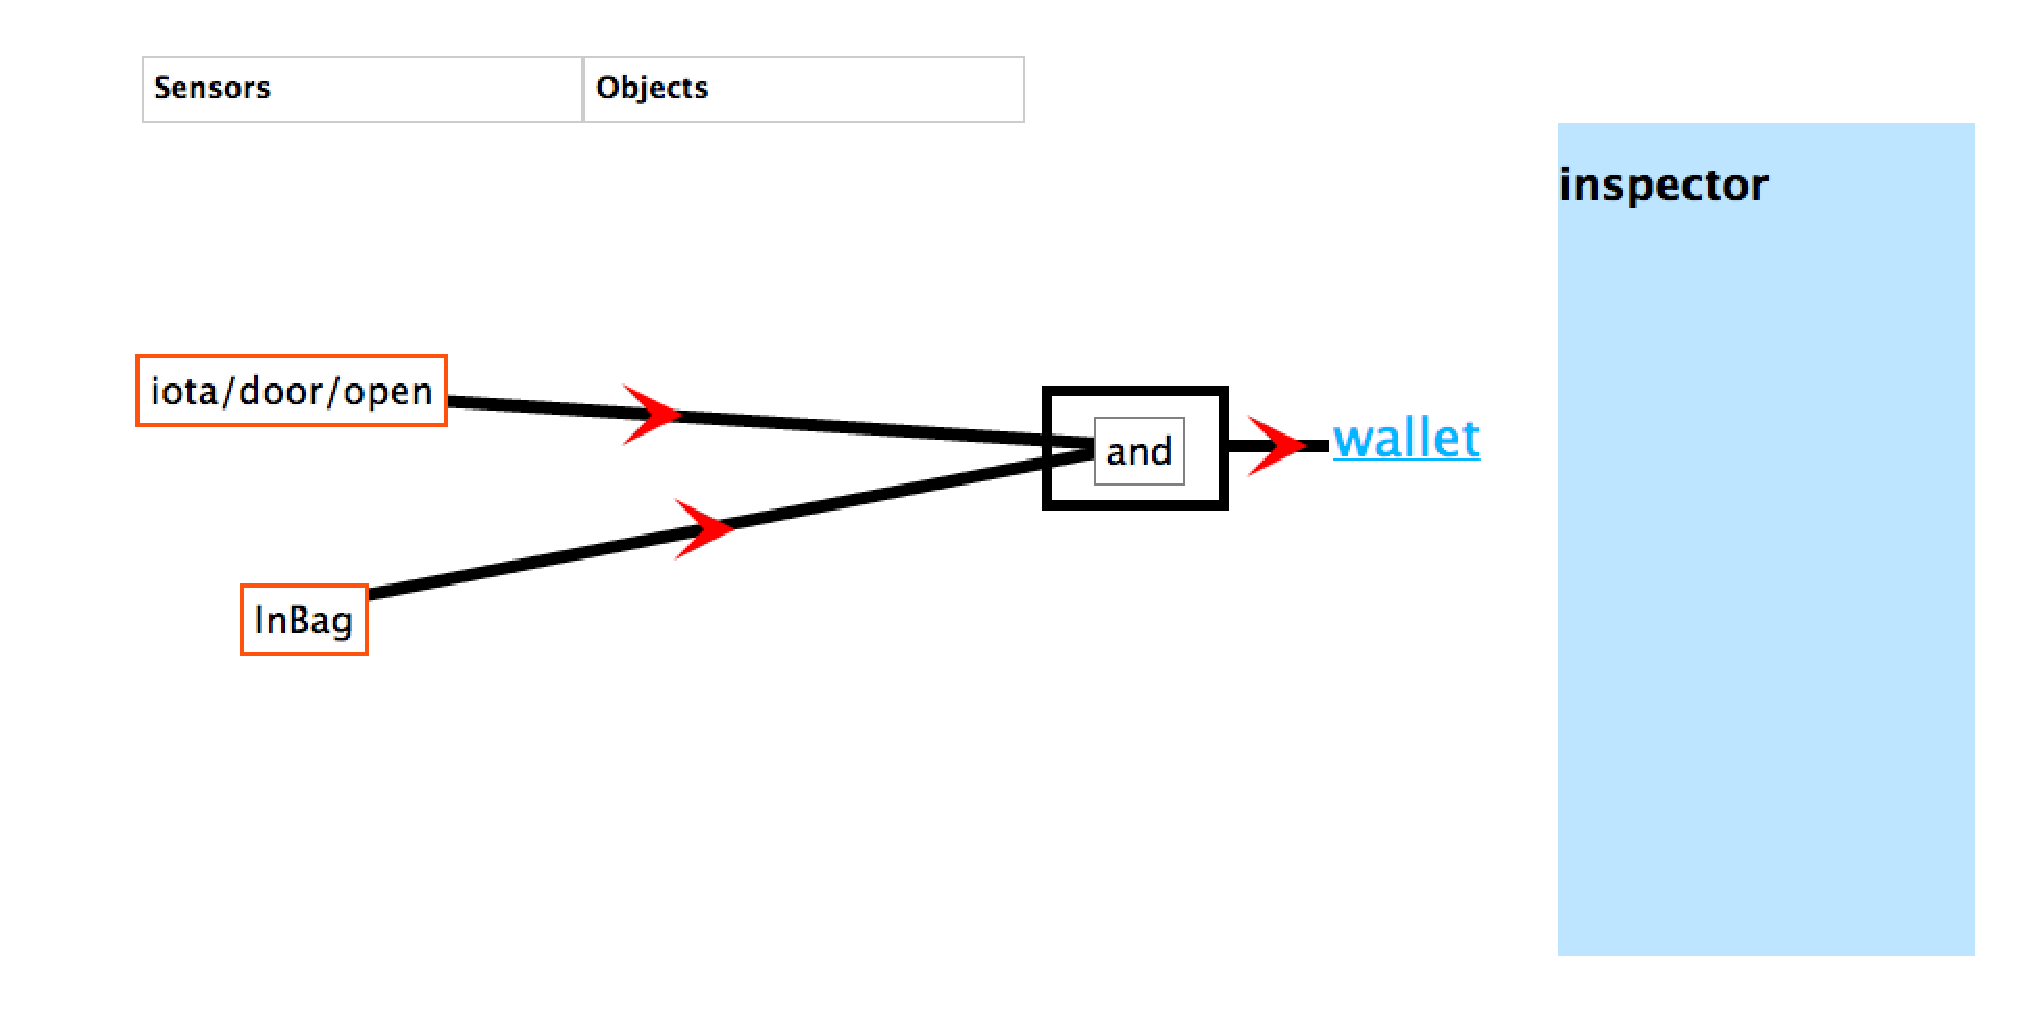
\includegraphics[width=150mm]{image/image12.eps}}
  \end{center}
  \caption{忘れ物検知をビジュアルプログラミング}
  \label{fig:image12}
\end{figure}

\section{カビを通知}
風呂場などに設置するといいだろう。その場所の温度と湿度をセンシングし、カビの発生条件に近いデータにマッチしたらイベントを発火する。また、壁を一定時間ごとに撮影し色の変化を観察することで精度をあげることが出来る。
(図\ref{fig:image13})では温度、湿度、壁の色という3つの要素でカビが発生しそうかどうか判定している。上から、温度20℃から30℃にマッチしたtrue、湿度が80%以上だったらtrue、壁の写真の色平均をとり、RGBの合計が100以下になったら黒ずんできたと判断しtrueとしている。
写真はRaspberry Pi\footnote{http://www.raspberrypi.org/}にWebカメラをつけ、定期的に色平均を計算させている。(図\ref{fig:image15})
\begin{figure}[htbp]
  \begin{center}
    \fbox{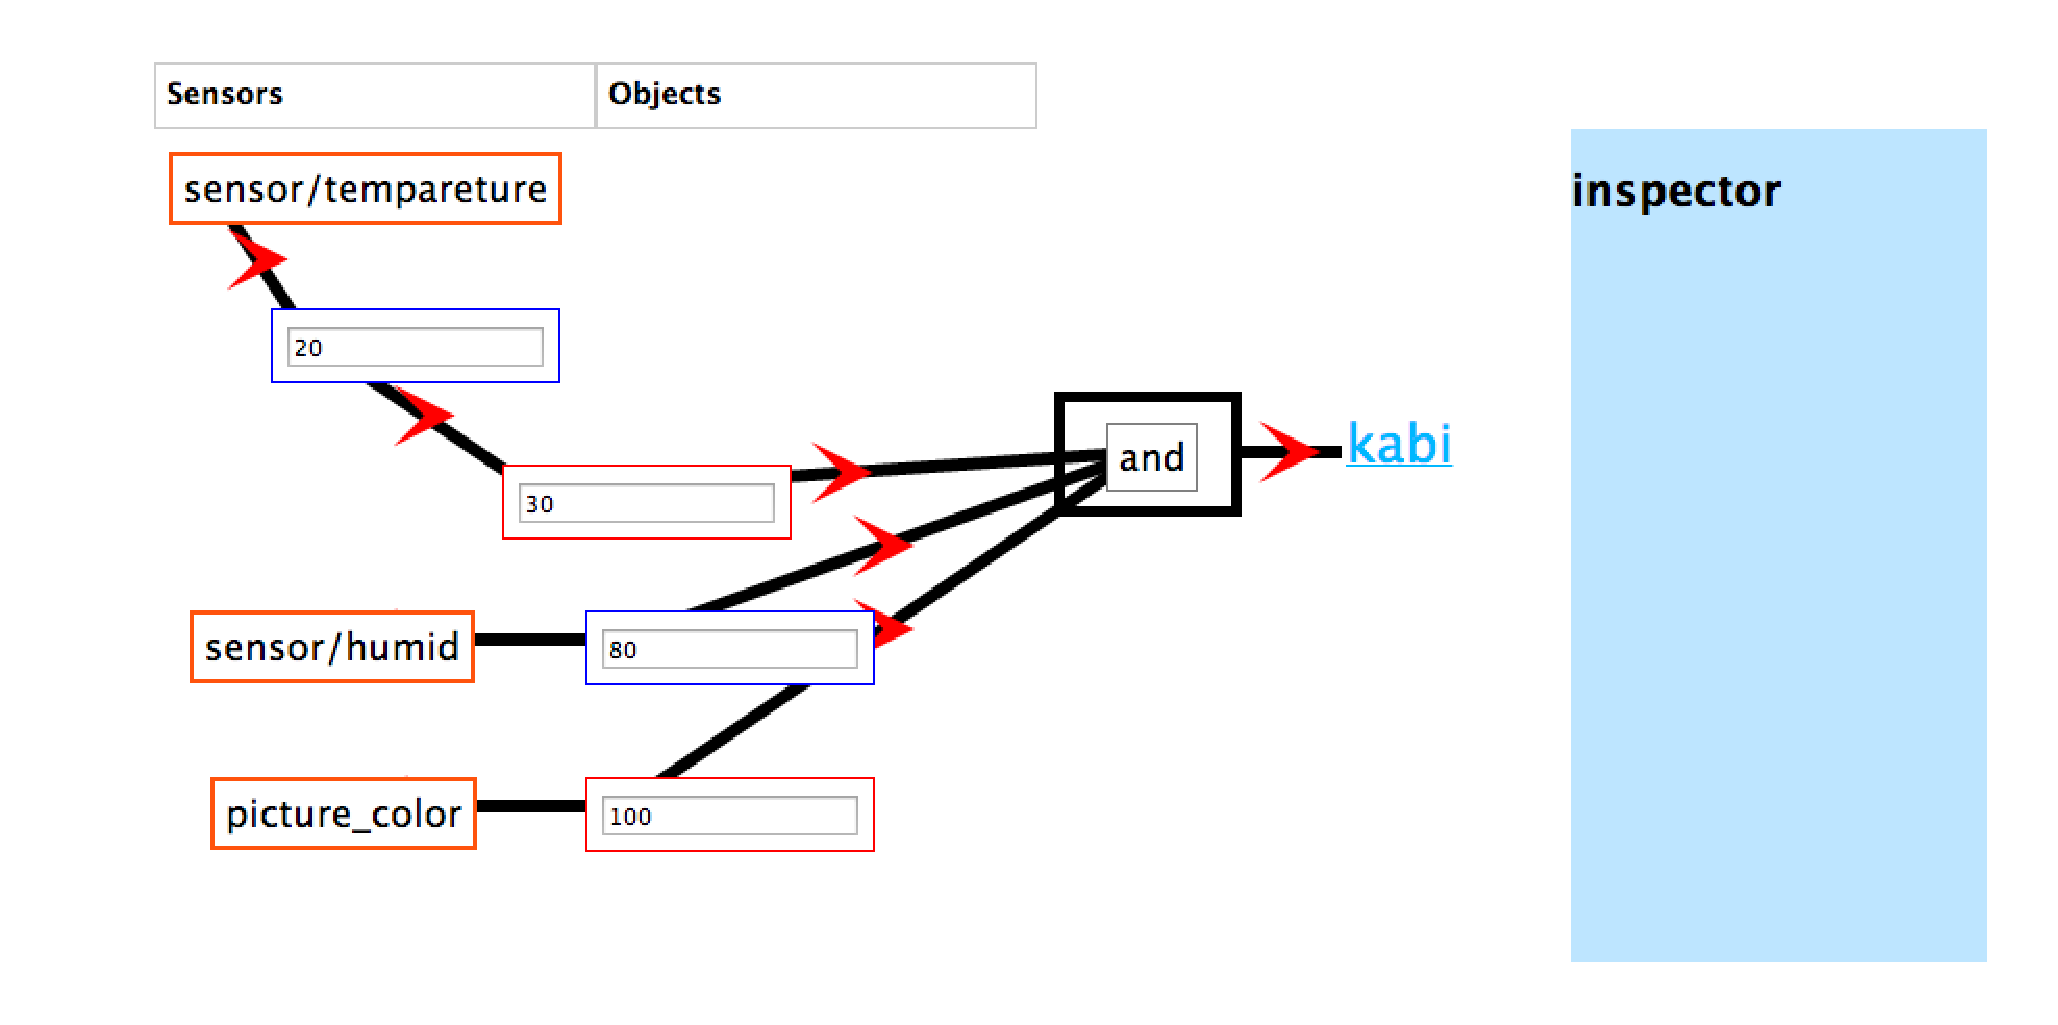
\includegraphics[width=150mm]{image/image13.eps}}
  \end{center}
  \caption{カビの通知をビジュアルプログラミング}
  \label{fig:image13}
\end{figure}

\begin{figure}[htbp]
  \begin{center}
    \fbox{\includegraphics[width=80mm]{image/image15.eps}}
  \end{center}
  \caption{壁の写真をとるための機構}
  \label{fig:image15}
\end{figure}

\section{朝食自動調理}
様々な条件に従って自動で料理を作ってくれるということも簡単にできるだろう。そもそも現状、炊飯器などにタイマーがついていて家電は色々な形で条件指定することができる。Web上で家電を管理することができれば人数や気温、季節、時間など複数の条件分岐を作成すれば複雑な条件で処理させることが可能だろう。
	% 本文4
\end{verbatim}
\end{itembox}

目次に続いて、論文のメイン、本文を記述する。アブストラクトと同様で、{\tt main.tex}に直接書くか、\verb|\include| コマンドを利用して別に用意したファイルを{\tt include}する。

本文の書き方は、第\ref{chap:latex}章で詳しく説明する。


\subsection{謝辞の出力}

\begin{itembox}[l]{{\tt main.tex}}
\begin{verbatim}
\begin{acknowledgment}
本研究を進めるにあたり、ご指導くださった増井俊之先生に深く感謝いたします。
アイデアの出し方、研究の進め方、実装方法など多くのことを学ばせていただきました。

橋本翔氏にはプログラミングの方法など、多くのことを学ばせて頂きました。ありがとうございました。

また、研究を進めるにあたり、増井研究室の皆様に多くのアドバイスを頂きました。心より感謝しております。\\\\
最後に学生生活を支えてくださった家族に感謝いたします。

\begin{flushright}
永倉 啓太
\end{flushright}

\end{acknowledgment}
	% 謝辞。要独自コマンド、include先参照のこと
\end{verbatim}
\end{itembox}

本文のあとには、謝辞を出力する。\verb|begin{acknowledgment}| から \verb|end{acknowledgment}| の間に書いた文章が、謝辞として独立したページに出力される。アブストラクトや本文と同じで、{\tt main.tex}に直接書いてもよいし、\verb|\include| コマンドを利用して{\tt include}してもよい。


\subsection{参考文献の出力}

\begin{itembox}[l]{{\tt main.tex}}
\begin{verbatim}
\include{91_bibliography}	% 参考文献。要独自コマンド、include先参照のこと
\end{verbatim}
\end{itembox}

謝辞に続いて、参考文献を出力する。

参考文献リストは、\verb|\begin{bib}| から \verb|\end{bib}| の間に、\verb|\bibitem| コマンドを使って書く。

BibTeXを使う場合は、以下のようにする。

\begin{itembox}[l]{{\tt 91\_bibliography.tex}}
\begin{verbatim}
\begin{bib}[100]
\bibliography{main}
\end{bib}
\end{verbatim}
\end{itembox}

こうすると、\verb|main.bib|から使用した参考文献のみを抽出して出力してくれる。\verb|main.bib|の中身は以下のようになっていて、気の利いた論文検索サイトであればBibTeXをコピペできるようになっているので簡単に作れるはず。


\begin{itembox}[l]{{\tt 91\_bibliography.tex}}
\begin{verbatim}
@article{hoge09,
    author  = "ほげ山太郎 and ほげ山次郎",
    yomi    = "ほげやまたろう",
    title   = "ほげほげ理論のHCI分野への応用",
    journal = "ほげほげ学会論文誌",
    volume  = "31",
    number  = "3",
    pages   = "194-201",
    year    = "2009",
}
@inproceedings{hoge08,
    author     = "Taro Hogeyama and Jiro Hogeyama",
    title      = "The Theory of Hoge",
    booktitle  = "The Proceedings of The Hoge Society",
    year       = "2008"
}
\end{verbatim}
\end{itembox}


以下は、BibTeXを使わないで手で書く例。

\begin{itembox}[l]{{\tt 91\_bibliography.tex}}
\begin{verbatim}
@article{hoge09,
    author  = "ほげ山太郎 and ほげ山次郎",
    yomi    = "ほげやまたろう",
    title   = "ほげほげ理論のHCI分野への応用",
    journal = "ほげほげ学会論文誌",
    volume  = "31",
    number  = "3",
    pages   = "194-201",
    year    = "2009",
}
@inproceedings{hoge08,
    author     = "Taro Hogeyama and Jiro Hogeyama",
    title      = "The Theory of Hoge",
    booktitle  = "The Proceedings of The Hoge Society",
    year       = "2008"
}
\end{verbatim}
\end{itembox}


英語の文献の場合、慣例的に書誌名をイタリック体にすることが多いらしい。

\begin{itembox}[l]{{\tt 91\_bibliography.tex}}
\begin{verbatim}
\begin{bib}[100]
\begin{thebibliography}{#1}
% \bibitem{参照用名称}
%   著者名:
%   \newblock 文献名,
%   \newblock 書誌情報,出版年.

\bibitem{hoge09}
  ほげ山太郎,ほげ山次郎:
  \newblock ほげほげ理論のHCI分野への応用,
  \newblock ほげほげ学会論文誌,Vol.31,No.3,pp.194-201,2009.

\bibitem{hoge08}
  Taro Hogeyama, Jiro Hogeyama:
  \newblock The Theory of Hoge,
  \newblock {\it The Proceedings of The Hoge Society}, 2008.
\end{thebibliography}
\end{bib}
\end{verbatim}
\end{itembox}

\verb|\bibitem| コマンド中、参照用名称は、本文から参考文献を参照するときに使うので、忘れずに書いておく。参照文献を本文中に参照するときには、\verb|\cite{参照用名称}| のように書けばよい。例えば、この文の末尾には \verb|\cite{hoge09}| と書いてあるので、自動で対応する番号が振られる\cite{hoge09}\cite{hoge08}。

参考文献リストの番号付けと、本文で参照したときの番号の挿入は、全部が自動で行われる。ただしこれも、第\ref{sec:toc}節で説明した目次の出力と同じで、一時ファイルを生成してからの挿入なので、正しく出力するには最低でも二回のコンパイルが必要。BibTeXを使用する場合は、\verb|platex|コマンドのあと\verb|pbibtex|コマンドを実行し、さらに2回\verb|platex|コマンドを実行するといいらしい。



\subsection{付録の出力}

\begin{itembox}[l]{{\tt main.tex}}
\begin{verbatim}
\appendix
\include{92_appendix}		% 付録
\end{verbatim}
\end{itembox}

必要であれば、論文の最後には付録を出力する。

\verb|\appendix| コマンド以降に書いたものは、すべて付録として扱われる。付録部分の書き方は通常の本文とまったく同じで、\verb|\appendix| コマンド以降に書くだけで勝手に付録用の体裁で出力される。
	% 本文2
\chapter{プロトタイプの実装}
\label{chap:prototype}

この章では本研究でのプロトタイプを実装し、その流れを解説する。

\section{実装概要}
大量のデータをやりとりすることを想定してnode.js\footnote{http://www.nodejs.org/}で実装した。またデータベースはmongoDB\footnote{http://www.mongodb.org/}を採用し、軽量フレームワークを実現した。元になっているセンサーデータはLindaを利用し、データを取得、書き込みしている。

クライアントサイドではJQuery UI\footnote{http://jqueryui.com/}とSVG\footnote{http://www.w3.org/Graphics/SVG/}を使い、ドラッグ&ドロップと線の描画を実現している。

\section{ページ遷移}
パスによってページを管理している。基本的にはパスの名前が最終的に結びつけるオブジェクトの名前になっている。パスにアクセスした際、オブジェクトが作成されていなかった場合には新しいオブジェクトの作成が促され、データベースに記録される。ユーザーはそのオブジェクトに対してアクションとその条件を指定することでプログラムしていく。/keyというページに最初にアクセスした際にはkeyオブジェクトを作成する。最終的なアクションは/key/outputでPOST送信先を設定する。例えば部屋の明るさをセンシングし、部屋が暗くなったらという条件をkeyオブジェクトに紐付け、携帯に通知を送るというアクションを実行することなどができる。その他にも鍵の開け閉めをWebで管理している場合にはそのURLにリクエストを送ることもできる。

/controlのパスはデータベースの管理ができるようになっており、センサーやオブジェクトに追加が出来るようになっている。


\section{サーバーサイド}
言語はJavascriptを使い、node.jsのsocket.io\footnote{http://socket.io/}で実装した。センサーオブジェクトに対して常にコネクションを貼り、データをemitしている。mongoDBではセンサーデータ、オブジェクトデータ、コネクションデータ、クライアントデータを保存している。

\section{クライアントサイド}
クライアントサイドもサーバーサイドと同様にJavascriptを選択した。ページ内でオブジェクトの作成、移動、コネクションの作成などのアクションが行われた際に常にサーバー側に情報を送り保存している。イベントの制御にはEvent Emitter\footnote{http://nodejs.org/api/events.html}を用いた。Event Emitterを使えばオブジェクト自体にイベントを持たせることができる。それぞれのオブジェクトが送られてきたデータを監視し、自分の持っている条件にマッチしたら自らが送信側になるという実装をしている。下の図ではdelta/sensor/lightというセンサーを親データとして、orというオブジェクトが監視して条件に照らし合わせマッチしたら発信するオブジェクトになっている。(図\ref{fig:image09})

\begin{figure}[htbp]
  \begin{center}
    \fbox{\includegraphics[width=100mm]{image/image09.eps}}
  \end{center}
  \caption{センサーデータの親子関係}
  \label{fig:image09}
\end{figure}

	% 本文3
\chapter{利用法}
\label{chap:usage}
この章ではセンシングデータの利用法を具体的に提案する。\\
センシングデータといってもWeb上で取得できる物は全てデータとして扱うことが出来る。
例えば藤沢の気温データをWeb上から更新される度に取得することで気温のセンシングデータを作成できる。また、現在時刻やPCのファイル情報などユーザーのコンテキストも取得してデータにすることが出来る。
これらのデータを使えば条件指定の幅が広がり複雑なプログラムを簡単に書くことが出来る。

\section{ニュース購読}
現在時刻を取得することで簡単にアラーム機能を実装できる。指定の時間をすぎるとニュースを取得し、PCに喋らせているのが以下の例だ。Macのsayコマンドを使って特定のPCから音声を発信している。
(図\ref{fig:image10})では時間を取得するtimeオブジェクトが9時と21時にマッチした時にnewsにアクセスしている。
\begin{figure}[htbp]
  \begin{center}
    \fbox{\includegraphics[width=150mm]{image/image10.eps}}
  \end{center}
  \caption{ニュースの購読をビジュアルプログラミング}
  \label{fig:image10}
\end{figure}

\section{超自動ドア}
携帯の位置情報とエレベーターで人があがってきたことをセンシングする。エレベーターがあがってきたという条件と携帯の位置が付近に来たことが送られてくると自動でドアが開く。(図\ref{fig:image14})のようにPOSTリクエストでドアをあける機構を作っておくことで実装可能だ。
(図\ref{fig:image11})はCellPhone\_lonというオブジェクトとCellPhone\_latというオブジェクトがそれぞれ緯度と経度を取得してきている。これをelevatorのデータとマージし、マッチした時にdoorにアクセスしている。
\begin{figure}[htbp]
  \begin{center}
    \fbox{\includegraphics[width=150mm]{image/image11.eps}}
  \end{center}
  \caption{超自動ドアをビジュアルプログラミング}
  \label{fig:image11}
\end{figure}

\begin{figure}[htbp]
  \begin{center}
    \fbox{\includegraphics[width=80mm]{image/image14.eps}}
  \end{center}
  \caption{自動解錠するための機構}
  \label{fig:image14}
\end{figure}

\section{忘れ物を通知}
ドアが開いたかどうか、と鞄の中に特定の物があるかというセンシングデータを組み合わせる。ドアが開いた時に鞄の中に物がなかった場合のみ通知をくるように設定し、忘れ物を防止することができる。
(図\ref{fig:image12})のInBagオブジェクトはRFIDタグ\footnote{固有のID情報を埋め込めるタグ}を鞄に設置し、登録した物の有無を検出する。一定時間でtrue/falseを判定し、trueの時だけイベントを発火する。そしてドアが開いた時に鞄の中の財布の有無を確認し、通知することができる。
\begin{figure}[htbp]
  \begin{center}
    \fbox{\includegraphics[width=150mm]{image/image12.eps}}
  \end{center}
  \caption{忘れ物検知をビジュアルプログラミング}
  \label{fig:image12}
\end{figure}

\section{カビを通知}
風呂場などに設置するといいだろう。その場所の温度と湿度をセンシングし、カビの発生条件に近いデータにマッチしたらイベントを発火する。また、壁を一定時間ごとに撮影し色の変化を観察することで精度をあげることが出来る。
(図\ref{fig:image13})では温度、湿度、壁の色という3つの要素でカビが発生しそうかどうか判定している。上から、温度20℃から30℃にマッチしたtrue、湿度が80%以上だったらtrue、壁の写真の色平均をとり、RGBの合計が100以下になったら黒ずんできたと判断しtrueとしている。
写真はRaspberry Pi\footnote{http://www.raspberrypi.org/}にWebカメラをつけ、定期的に色平均を計算させている。(図\ref{fig:image15})
\begin{figure}[htbp]
  \begin{center}
    \fbox{\includegraphics[width=150mm]{image/image13.eps}}
  \end{center}
  \caption{カビの通知をビジュアルプログラミング}
  \label{fig:image13}
\end{figure}

\begin{figure}[htbp]
  \begin{center}
    \fbox{\includegraphics[width=80mm]{image/image15.eps}}
  \end{center}
  \caption{壁の写真をとるための機構}
  \label{fig:image15}
\end{figure}

\section{朝食自動調理}
様々な条件に従って自動で料理を作ってくれるということも簡単にできるだろう。そもそも現状、炊飯器などにタイマーがついていて家電は色々な形で条件指定することができる。Web上で家電を管理することができれば人数や気温、季節、時間など複数の条件分岐を作成すれば複雑な条件で処理させることが可能だろう。
	% 本文4
\end{verbatim}
\end{itembox}

目次に続いて、論文のメイン、本文を記述する。アブストラクトと同様で、{\tt main.tex}に直接書くか、\verb|\include| コマンドを利用して別に用意したファイルを{\tt include}する。

本文の書き方は、第\ref{chap:latex}章で詳しく説明する。


\subsection{謝辞の出力}

\begin{itembox}[l]{{\tt main.tex}}
\begin{verbatim}
\begin{acknowledgment}
本研究を進めるにあたり、ご指導くださった増井俊之先生に深く感謝いたします。
アイデアの出し方、研究の進め方、実装方法など多くのことを学ばせていただきました。

橋本翔氏にはプログラミングの方法など、多くのことを学ばせて頂きました。ありがとうございました。

また、研究を進めるにあたり、増井研究室の皆様に多くのアドバイスを頂きました。心より感謝しております。\\\\
最後に学生生活を支えてくださった家族に感謝いたします。

\begin{flushright}
永倉 啓太
\end{flushright}

\end{acknowledgment}
	% 謝辞。要独自コマンド、include先参照のこと
\end{verbatim}
\end{itembox}

本文のあとには、謝辞を出力する。\verb|begin{acknowledgment}| から \verb|end{acknowledgment}| の間に書いた文章が、謝辞として独立したページに出力される。アブストラクトや本文と同じで、{\tt main.tex}に直接書いてもよいし、\verb|\include| コマンドを利用して{\tt include}してもよい。


\subsection{参考文献の出力}

\begin{itembox}[l]{{\tt main.tex}}
\begin{verbatim}
\include{91_bibliography}	% 参考文献。要独自コマンド、include先参照のこと
\end{verbatim}
\end{itembox}

謝辞に続いて、参考文献を出力する。

参考文献リストは、\verb|\begin{bib}| から \verb|\end{bib}| の間に、\verb|\bibitem| コマンドを使って書く。

BibTeXを使う場合は、以下のようにする。

\begin{itembox}[l]{{\tt 91\_bibliography.tex}}
\begin{verbatim}
\begin{bib}[100]
\bibliography{main}
\end{bib}
\end{verbatim}
\end{itembox}

こうすると、\verb|main.bib|から使用した参考文献のみを抽出して出力してくれる。\verb|main.bib|の中身は以下のようになっていて、気の利いた論文検索サイトであればBibTeXをコピペできるようになっているので簡単に作れるはず。


\begin{itembox}[l]{{\tt 91\_bibliography.tex}}
\begin{verbatim}
@article{hoge09,
    author  = "ほげ山太郎 and ほげ山次郎",
    yomi    = "ほげやまたろう",
    title   = "ほげほげ理論のHCI分野への応用",
    journal = "ほげほげ学会論文誌",
    volume  = "31",
    number  = "3",
    pages   = "194-201",
    year    = "2009",
}
@inproceedings{hoge08,
    author     = "Taro Hogeyama and Jiro Hogeyama",
    title      = "The Theory of Hoge",
    booktitle  = "The Proceedings of The Hoge Society",
    year       = "2008"
}
\end{verbatim}
\end{itembox}


以下は、BibTeXを使わないで手で書く例。

\begin{itembox}[l]{{\tt 91\_bibliography.tex}}
\begin{verbatim}
@article{hoge09,
    author  = "ほげ山太郎 and ほげ山次郎",
    yomi    = "ほげやまたろう",
    title   = "ほげほげ理論のHCI分野への応用",
    journal = "ほげほげ学会論文誌",
    volume  = "31",
    number  = "3",
    pages   = "194-201",
    year    = "2009",
}
@inproceedings{hoge08,
    author     = "Taro Hogeyama and Jiro Hogeyama",
    title      = "The Theory of Hoge",
    booktitle  = "The Proceedings of The Hoge Society",
    year       = "2008"
}
\end{verbatim}
\end{itembox}


英語の文献の場合、慣例的に書誌名をイタリック体にすることが多いらしい。

\begin{itembox}[l]{{\tt 91\_bibliography.tex}}
\begin{verbatim}
\begin{bib}[100]
\begin{thebibliography}{#1}
% \bibitem{参照用名称}
%   著者名:
%   \newblock 文献名,
%   \newblock 書誌情報,出版年.

\bibitem{hoge09}
  ほげ山太郎,ほげ山次郎:
  \newblock ほげほげ理論のHCI分野への応用,
  \newblock ほげほげ学会論文誌,Vol.31,No.3,pp.194-201,2009.

\bibitem{hoge08}
  Taro Hogeyama, Jiro Hogeyama:
  \newblock The Theory of Hoge,
  \newblock {\it The Proceedings of The Hoge Society}, 2008.
\end{thebibliography}
\end{bib}
\end{verbatim}
\end{itembox}

\verb|\bibitem| コマンド中、参照用名称は、本文から参考文献を参照するときに使うので、忘れずに書いておく。参照文献を本文中に参照するときには、\verb|\cite{参照用名称}| のように書けばよい。例えば、この文の末尾には \verb|\cite{hoge09}| と書いてあるので、自動で対応する番号が振られる\cite{hoge09}\cite{hoge08}。

参考文献リストの番号付けと、本文で参照したときの番号の挿入は、全部が自動で行われる。ただしこれも、第\ref{sec:toc}節で説明した目次の出力と同じで、一時ファイルを生成してからの挿入なので、正しく出力するには最低でも二回のコンパイルが必要。BibTeXを使用する場合は、\verb|platex|コマンドのあと\verb|pbibtex|コマンドを実行し、さらに2回\verb|platex|コマンドを実行するといいらしい。



\subsection{付録の出力}

\begin{itembox}[l]{{\tt main.tex}}
\begin{verbatim}
\appendix
\include{92_appendix}		% 付録
\end{verbatim}
\end{itembox}

必要であれば、論文の最後には付録を出力する。

\verb|\appendix| コマンド以降に書いたものは、すべて付録として扱われる。付録部分の書き方は通常の本文とまったく同じで、\verb|\appendix| コマンド以降に書くだけで勝手に付録用の体裁で出力される。
